
\documentclass[10pt, compress, aspectratio=169]{beamer}
\usetheme{metropolis}
\usepackage{bm}
\usepackage{booktabs}
\usepackage{tikz}
\usetikzlibrary{arrows.meta}
\usepackage{multirow, multicol}
\usepackage{tabularx}
\usepackage{makecell}
\usepackage[scale=2]{ccicons}
\usepackage{subcaption}
\usepackage{xcolor}
\usepackage{colortbl} 
\usepackage[linesnumbered,lined,boxed,commentsnumbered, ruled,vlined]{algorithm2e}
\DeclareRobustCommand{\mythead}[1]{%
  \begin{tabular}{@{}l@{}}#1\end{tabular}%
}
\usepackage{tikz}
\usepackage{amsmath}
\usetikzlibrary{arrows,shapes}

\usepackage{tabularray}
\UseTblrLibrary{varwidth}


\definecolor{mygreen}{RGB}{0, 102, 0}
\newcommand\ytl[2]{
\parbox[b]{3em}{\hfill{\color{cyan}\bfseries\sffamily #1}~$\cdots$~}\makebox[0pt][c]{$\bullet$}\vrule\quad \parbox[c]{8.5cm}{\vspace{7pt}\color{red!40!black!80}\raggedright\sffamily #2.\\[7pt]}\\[-3pt]}

\usepackage{mathtools}
\DeclarePairedDelimiter{\nint}\lfloor\rceil
\DeclarePairedDelimiter{\ceil}{\lceil}{\rceil}
\DeclarePairedDelimiter{\abs}\lvert\rvert

\newcommand\marklessfootnote[1]{
    \addtocounter{footnote}{1} %no call is made to \footnotemark.
    \footnotetext{#1}
  }
  
\newcommand{\highlighti}[2]{%
    \setlength{\fboxrule}{2pt}%
    \fcolorbox{#1}{white}{#2}}



\title{An Isomorphic Transformation for Hardware Implemented Non-negative Neural Networks}
\author{{\Book\bfseries Manos Kirtas}\inst{1, 2}, Nikolaos Passalis\inst{1}, Nikos Pleros\inst{1}, Anastasios Tefas\inst{1}}
\date{27 May 2027}
\institute{\inst{1}Aristotle University of Thessaloniki, Greece \and \inst{2}Centre de Nanosciences et de Nanotechnologies, CNRS, France }

\begin{document}
\tikzstyle{every picture}+=[remember picture]
% \everymath{\displaystyle}

{
\setbeamerfont{title}{size=\LARGE, series=\bfseries}
\setbeamercolor{title}{fg=white}
\setbeamercolor{title separator}{fg=white}
\setbeamercolor{author}{fg=white}
\setbeamercolor{institute}{fg=white}
\setbeamercolor{date}{fg=white}
\setbeamertemplate{author}{
  \vspace*{0.1em}
  \insertauthor\par
  \vspace*{0.1em}
}
\usebackgroundtemplate{%
  
\includegraphics[width=\paperwidth,height=\paperheight]{images/iscas26_background_front.pdf}%
}
\frame
{
    \vspace{55pt}
    \titlepage
    \begin{tikzpicture}[remember picture, overlay]
      \node[anchor=south east, xshift=-6pt, yshift=6pt] at (current page.south east) {
        
\includegraphics[height=1.2cm]{images/SYMPHONY-LOGO.png}
        \hspace{4pt}
        
\includegraphics[height=1.2cm]{images/LogoAUTHwhite300ppi.png}
        \hspace{4pt}
        
\includegraphics[height=1.2cm]{images/c2n.png}
        \hspace{4pt}
        
\includegraphics[height=1.2cm]{images/LOGO_CNRS_BLANC.png}
        };
    \end{tikzpicture}
}
}

\usebackgroundtemplate{%
  
\includegraphics[width=\paperwidth,height=\paperheight]{images/iscas26_background_general.pdf}%
}

\section{Introduction}


%%%%%%%%%%%%%%%%%%%%%%%%%%%%%%%%%%%%%%%%%%%%%%%%%%%%%%%%%%%%%%%%%%%%%%%%%%%%%%%%%%%%%%%%%%%%%%%%%%%% 
\begin{frame}{Computation Demands}
\begin{columns}[c]
  \begin{column}{0.5\textwidth}
    Over the last 15 years, the required \textbf{training computations have been approximately doubled every 6 months.}

    \vspace{20pt}

    This indicates the \textbf{synergistic advances achieved} in both deep learning
    \textbf{methodologies} and \textbf{hardware}
    capabilities.\footnotemark
  \end{column}
  \begin{column}{0.5\textwidth}
    \begin{center}
      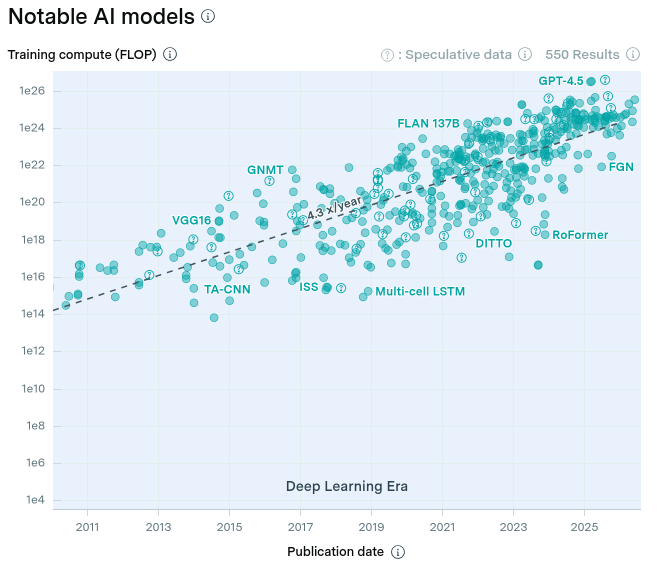
\includegraphics[width=\linewidth]{sections/0_intro/imgs/epoch-ml-trends-2.png}
    \end{center}
  \end{column}
\end{columns}
\footnotetext{\textbf{Source:} Sevilla, Jaime, et al. "Compute trends
  across three eras of machine learning." 2022 International Joint Conference on
  Neural Networks (IJCNN). IEEE, 2022. (https://epoch.ai/blog/compute-trends)}
\end{frame}

%%%%%%%%%%%%%%%%%%%%%%%%%%%%%%%%%%%%%%%%%%%%%%%%%%%%%%%%%%%%%%%%%%%%%%%%%%%%%%%%%%%%%%%%%%%%%%%%%%%% 

\begin{frame}{Hardware Accelerator}
\begin{itemize}
    \item \textbf{Pushing the boundaries of available hardware}
    \item Reveals the need to \textbf{shift towards specialized hardware}
\end{itemize} \vspace{15pt}

    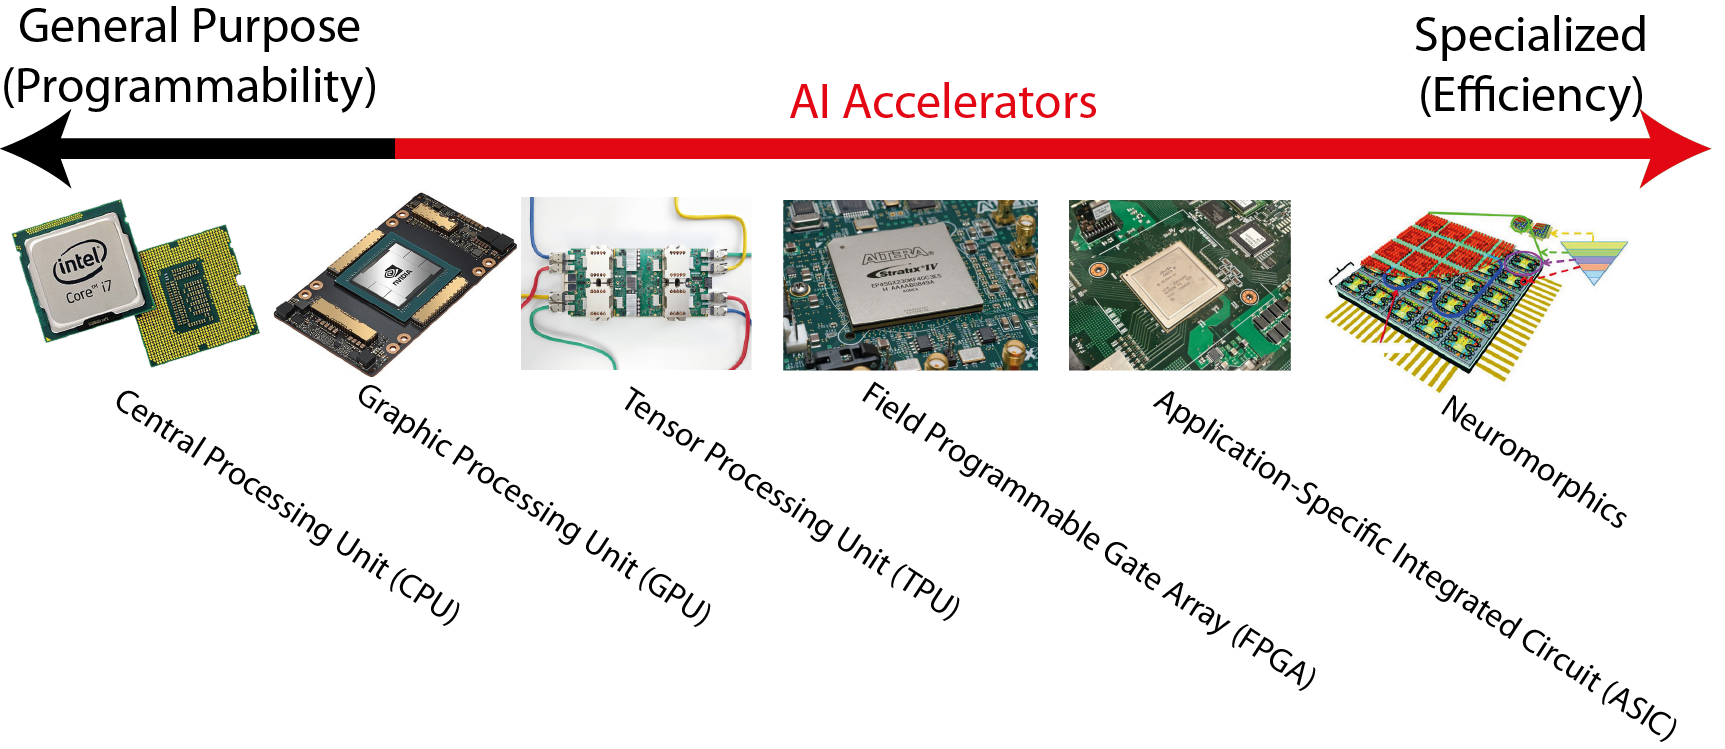
\includegraphics[width=0.9\linewidth]{sections/0_intro/imgs/intro_phd.png}
\end{frame}

%%%%%%%%%%%%%%%%%%%%%%%%%%%%%%%%%%%%%%%%%%%%%%%%%%%%%%%%%%%%%%%%%%%%%%%%%%%%%%%%%%%%%%%%%%%%%%%%%%%% 


\begin{frame}{Integrated Silicon Photonics}
  \textbf{Photonic neurons encode signal using light},  which are then manipulated to provide functionality in neurons. \vspace{-5pt}
  % rather than electric quantities,
  % Providing a great potential to be used in DL accelerators due to:
  \begin{center}
    \begin{figure}
        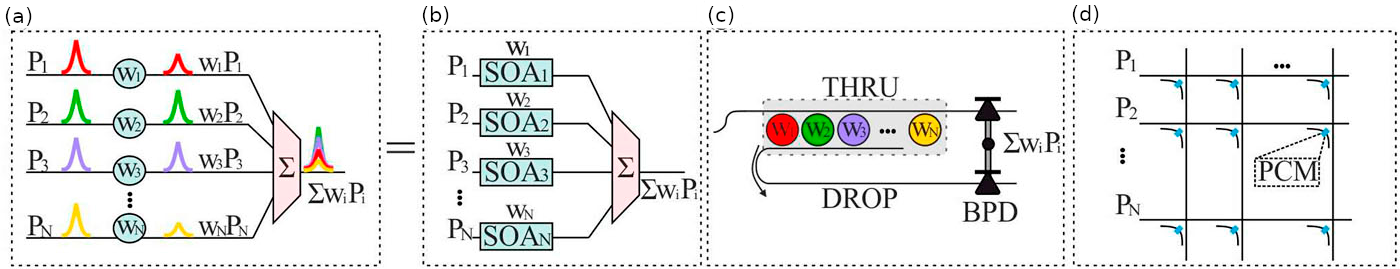
\includegraphics[width=\linewidth]{sections/0_intro/imgs/apl_incoherent.png}
        \caption{Indicative layouts adopt the incoherent
          concept.\footnote{\textbf{Source:} Tsakyridis, A., Moralis-Pegios, M., Giamougiannis, G., Kirtas, M., Passalis, N., Tefas, A. and Pleros, N., 2024. Photonic neural networks and optics-informed deep learning fundamentals. APL photonics, 9(1).} \vspace{-5pt}}
    \end{figure}
  \end{center}
  A majority of currently available \textbf{photonic architectures rely on incoherent layouts}.
\end{frame}

%%%%%%%%%%%%%%%%%%%%%%%%%%%%%%%%%%%%%%%%%%%%%%%%%%%%%%%%%%%%%%%%%%%%%%%%%%%%%%%%%%%%%%%%%%%%%%%%%%%%
\begin{frame}{Incoherent Photonics \& The Sign Problem}

\begin{columns}[T]

%% ── LEFT COLUMN ─────────────────────────────────────────────
\begin{column}{0.46\textwidth}
  \vspace{0.1em}
  In incoherent photonics the  optical signals are converted into
  \textbf{power signals} during the activation stage.

    % ── wave picture ────────────────────────────────────────────
  \begin{center}
  \begin{tikzpicture}[scale=0.78, >=stealth]

    %% axes
    \draw[->] (-0.3,0) -- (5.6,0) node[right,font=\small] {$t$};
    \draw[->] (0,-1.5) -- (0, 2.4) node[above,font=\small] {$E(t),\; \sum_{\forall i}E_i(t),\; \sum_{\forall i}|E_{i}|^2$};

    %% electric field  E(t) = sin
    \draw[blue!70!black, thick, domain=0:5.4, samples=120]
      plot (\x, {1.1*sin(360*\x/2.2)})
      node[right, font=\tiny, blue!70!black] {$\sum_{i=0}^{n}E_{i}(t)$};

    %% incoherent intensities — three sources with random phases
    \draw[red!70!black, thick, opacity=0.4, domain=0:5.4, samples=120]
      plot (\x, {1.1*(sin(360*\x/2.2))})
      node[right, font=\tiny, red!70!black, opacity=1] {$E_1$};
    \draw[orange!70!black, thick, opacity=0.44, domain=0:5.4, samples=120]
      plot (\x, {1.1*(sin(360*\x/2.2+80))})
      node[right, font=\tiny, orange!70!black, opacity=1] {$E_2$};
    \draw[violet!70!black, thick, opacity=0.44, domain=0:5.4, samples=120]
      plot (\x, {1.1*(sin(360*\x/2.2+160))})
      node[right, font=\tiny, violet!70!black, opacity=1] {$E_3$};

    %% I_total = Σ|E_i|²  (incoherent: no cross-terms)
    \draw[red!80!black, very thick, domain=0:5.4, samples=120]
      plot (\x, {1* ((sin(360*\x/2.2))^2+(sin(360*\x/2.2+80))^2+(sin(360*\x/2.2+160))^2)})
      node[right, font=\tiny, red!80!black] {$\sum_{i=0}^{n}|E_{i}|^{2}(t)$};

    %% forbidden zone label
    \fill[red!12, opacity=0.3] (-0.2,-1.45) rectangle (5.55,-0.02);
    \draw[red!40, dashed] (-0.2,-0.02) -- (5.55,-0.02);
    \node[font=\tiny, red!60!black] at (2.7,-0.75)
      {forbidden region ($I < 0$ impossible)};

    %% annotation arrows
    % \draw[->, gray, thin] (1.35,1.45)
    %   to[bend left=20] node[midway, right, font=\tiny]{$\scriptstyle |E|^2$}
    %   (1.55,0.95);
    \end{tikzpicture}
  \end{center}

  \vspace{1.2em}
\end{column}

\hfill
%% ── RIGHT COLUMN ────────────────────────────────────────────
\begin{column}{0.50\textwidth}
  An electromagnetic wave propagating in a medium has an electric field:
  \[E(r, t) = A e^{i(kr - \omega t)}\]

  A photodetector measures the optical intensity:
  \[
    I = \tfrac{1}{2}\,\varepsilon_0 c\,|E|^2 \;\geq\; 0
  \]
  The generated photocurrent given by
  \[
    i_{\mathrm{ph}} = \mathcal{R}\cdot P = \mathcal{R}
    \int_{\!\mathcal{A}} I\,\mathrm{d}A \;\geq\; 0
  \]


  % \vspace{0.3em}
  % \centering
  % \begin{tabular}{@{}lcc@{}}
  %   \hline
  %   \textbf{Quantity} & \textbf{Range} & \textbf{Signed?} \\
  %   \hline
  %   Field $E$          & $\mathbb{R}$   & \textcolor{green!60!black}{\checkmark} \\
  %   Intensity $|E|^2$  & $[0,+\infty)$ & \textcolor{red}{\texttimes} \\
  %   Photocurrent $i_{\mathrm{ph}}$ & $[0,+\infty)$ & \textcolor{red}{\texttimes} \\
  %   \hline
  % \end{tabular}

\end{column}
\end{columns}
\vspace{-20pt}
\begin{center}
  \color{red}{\textbf{Sign information} of the weighted sum is ignored.}
\end{center}
\end{frame}

%%%%%%%%%%%%%%%%%%%%%%%%%%%%%%%%%%%%%%%%%%%%%%%%%%%%%%%%%%%%%%%%%%%%%%%%%%%%%%%%%%%%%%%%%%%%%%%%%%%%

\begin{frame}{Motivation}
  This makes the use of negative representations a challenging process,
  typically enforcing the adoption of higher complexity hardware architectures
  (e.x. balanced photodetectors).

  \vspace{10pt}
  % , such as balanced photodetector schemes,
  % biasing configurations and signal transformation blocks. 

  To overcome this, one can train non-negative neural networks, however
  \begin{itemize}
  \item Current available methods target \textbf{partial non-negative architectures}
  \item Applied on \textbf{small datasets} or \textbf{non-traditionally used ANNs}
  \item \textbf{Facing difficulties in scaling} ability and \textbf{generalization} in DL architectures
  \item Results in \textbf{performance degradation}
  \end{itemize}  
\end{frame}

% \section{Robust and Noise Resilient Training}

\begin{frame}{Easily Saturated Photonic Activation Functions}
  % The unique nature of optical non-linearities:
  \begin{center}
       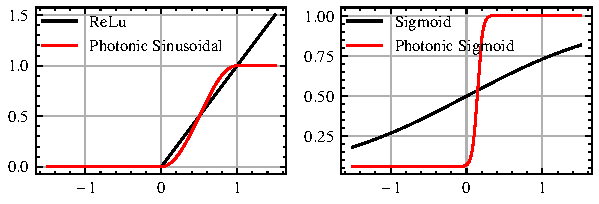
\includegraphics[width=0.9\textwidth]{./sections/1_adaptinit/imgs/activations.pdf}
  \end{center} \vspace{-10pt}
  \begin{itemize}
  \item \textcolor{red}{Facing challenges to support traditionally used activation functions such as ReLu}
  \item \textcolor{red}{Mostly relying on high slope functions such as
      sinusoidal- or sigmoidal-based}
  \end{itemize}
\end{frame}


\begin{frame}{Vanishing Gradients}
\begin{center}
    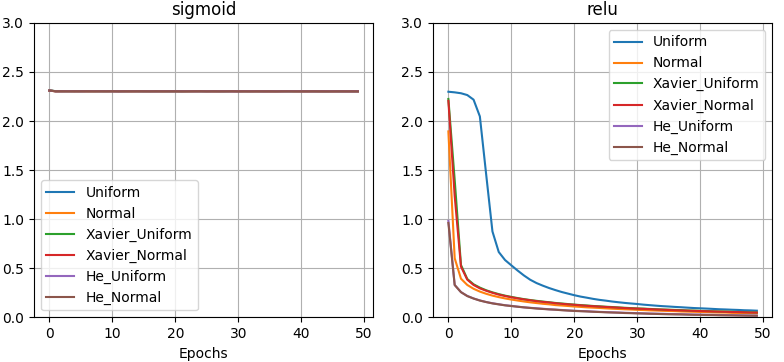
\includegraphics[width=0.9\textwidth]{./sections/1_adaptinit/imgs/specific_initialization.png}
\end{center}
    \begin{itemize}
        \item \textbf{Susceptible to vanishing gradient phenomena}
        \item \textbf{Making PNNs especially sensitive to the initialization scheme} 
    \end{itemize}
\end{frame}


\begin{frame}{Typically Weights Initialization}

  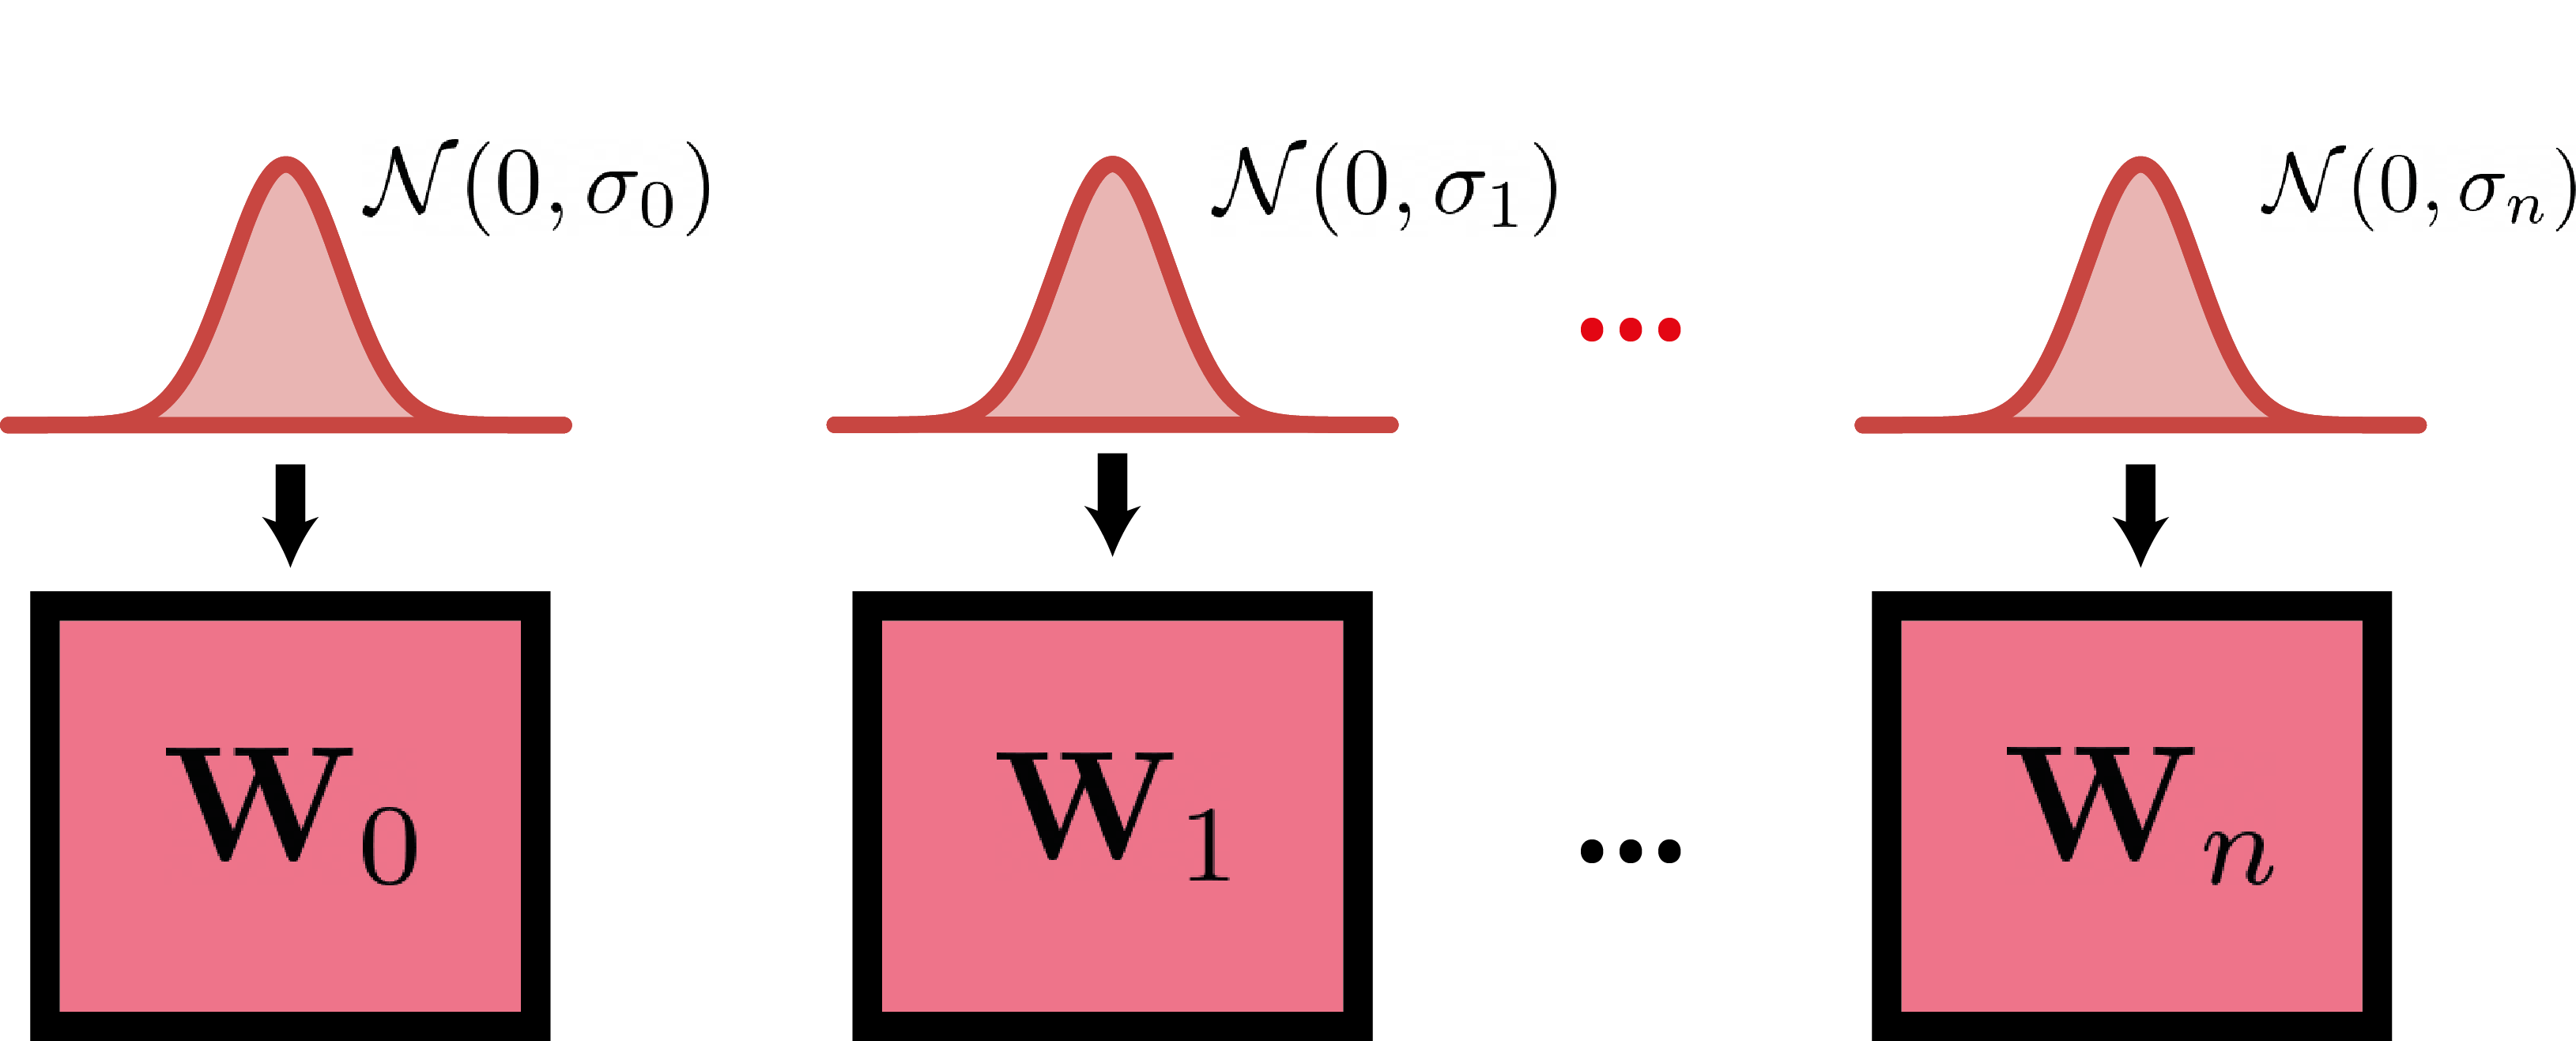
\includegraphics[width=\linewidth]{sections/1_adaptinit/imgs/adapt_init_1.png} \vspace{10pt}
  
    Typically the \textbf{weights of \(i\)-th layer are initialized by
    drawing from a Gaussian distribution} with zero mean and \(\sigma^2_i
  \in \mathbb{R}\) variance, denoted by $\mathbf{W}_i \sim
  \mathcal{N}_{N_{i} \times N_{i-1}}(0,
  \sigma^2_i)$. 
\end{frame}

\begin{frame}{Limitation of Initialization methods} % Here I can also add Xavier and He initialization
    \textbf{Vanishing gradient phenomena have been extensively studied for regular training}.
    \begin{itemize}
        \item \textcolor{red}{Such schemes target traditionally used activation functions}
        \item \textcolor{red}{Consider only the size of every layer (fan-in and fan-out)}
        \item \textcolor{red}{Ignoring the synergistic effects during inference (such as noise)}
    \end{itemize}
    \textcolor{red}{\textbf{Leading to suboptimal results and limiting the performance of models in such systems.}}
  \end{frame}


\begin{frame}{Thesis Contribution}
  An unified \textbf{hardware-aware training framework} that incorporates: 
  \begin{itemize}
    \item \textbf{Photonic transfer functions} in the optical configuration
    \item Easily saturated \textbf{photonic activation functions}
    \item Inevitable \textbf{noise sources} exists during hardware inference
    \end{itemize}
    
    % The proposed method is an \textbf{architecture-agnostic} method that
    % deals with both \textbf{initialization of trainable parameters} and actual \textbf{weight
    % update} in gradient-based optimization.

    % Establishing a more holistic co-design approach in training process. 
\end{frame}


% \begin{frame}{Establishing Objective}
% 	The information flow through network can be theoretically modeled by the
%   Markov chain rule: 
%   \begin{equation}
%     Y \rightarrow X \rightarrow \hat{X}_1  \rightarrow \dots \rightarrow \hat{X}_M \rightarrow \hat{Y},
%   \end{equation}
%   {\scriptsize   where \(X\) be the input random variable (input to the ANN), Y the target variable,
%   and \(\hat{Y}\) the final network prediction as acquired through a series of
%   layer transformations \(\hat{X}_1, \dots \hat{X}_M\). } \vspace{15pt}

%     
\includegraphics[width=0.9\linewidth]{sections/1_adaptinit/imgs/info_0.png}

% \end{frame}


% \begin{frame}{Suboptimal Initialization}

%   The information lost in one layer cannot be recovered later in subsequent
%   layers.
%   \begin{equation}
%     I(Y; X) \geq I(Y; \hat{X}_1) \geq \dots \geq I(Y; \hat{X}_M) \geq I(Y;\hat{Y}).
%   \end{equation} \vspace{15pt}

%   
\includegraphics[width=\linewidth]{sections/1_adaptinit/imgs/info_1.png}

% 	% Now suppose that due to a suboptimal initialization scheme, we have suppressed
%   % most information about \(Y\) in the first layer, i.e., \(I(Y; \hat{X}_1) =
%   % \epsilon\). Then this implies that:
%   % \begin{equation}
%   %   I(Y; \hat{Y}) \leq I(Y; \hat{X}_M) \leq  \dots \leq I(Y; \hat{X}_2) = \epsilon.
%   % \end{equation}
%   % Therefore, we cannot retrieve any
%   % additional information about \(Y\) after this layer.
% \end{frame}

% \begin{frame}{Initialization Objective}
% 	% Also, note that ``compressing'' in such a way that irrelevant information
%   % about \(Y\) is beneficial, since it allows us to acquire representations that
%   % discard irrelevant information and keep only the factors that explain \(Y\).
%   % Deep Learning process can be seen as a process of finding approximate minimal
%   % sufficient statistics about \(Y\),  
%   % \[\mathcal{L} = I(X; \hat{Y}) - \alpha I(Y; \hat{Y}),\] where \(\alpha\)
%   % controls the trade-off between the compression rate and the information
%   % preserved about \(Y\).

%     The initialization can be formulated as an optimization problem that targets
%     maximize the information for the \(k\)-th layer: 
%     \begin{equation}
%      \begin{aligned}
%          \text{maximize } \quad &  I(Y_k, \hat{Y}), \text{ }  \forall k \in [0, M],\\
%          \text{s.t. } \quad &  \bm{W}_{k} \sim N(0,a_k\sigma^2), \\
%          & a_k > 0, \\
%     \end{aligned}
%   \end{equation}
%   {\scriptsize where \(M \in \mathbb{N}\) is the number of layers.} \vspace{15pt}

%  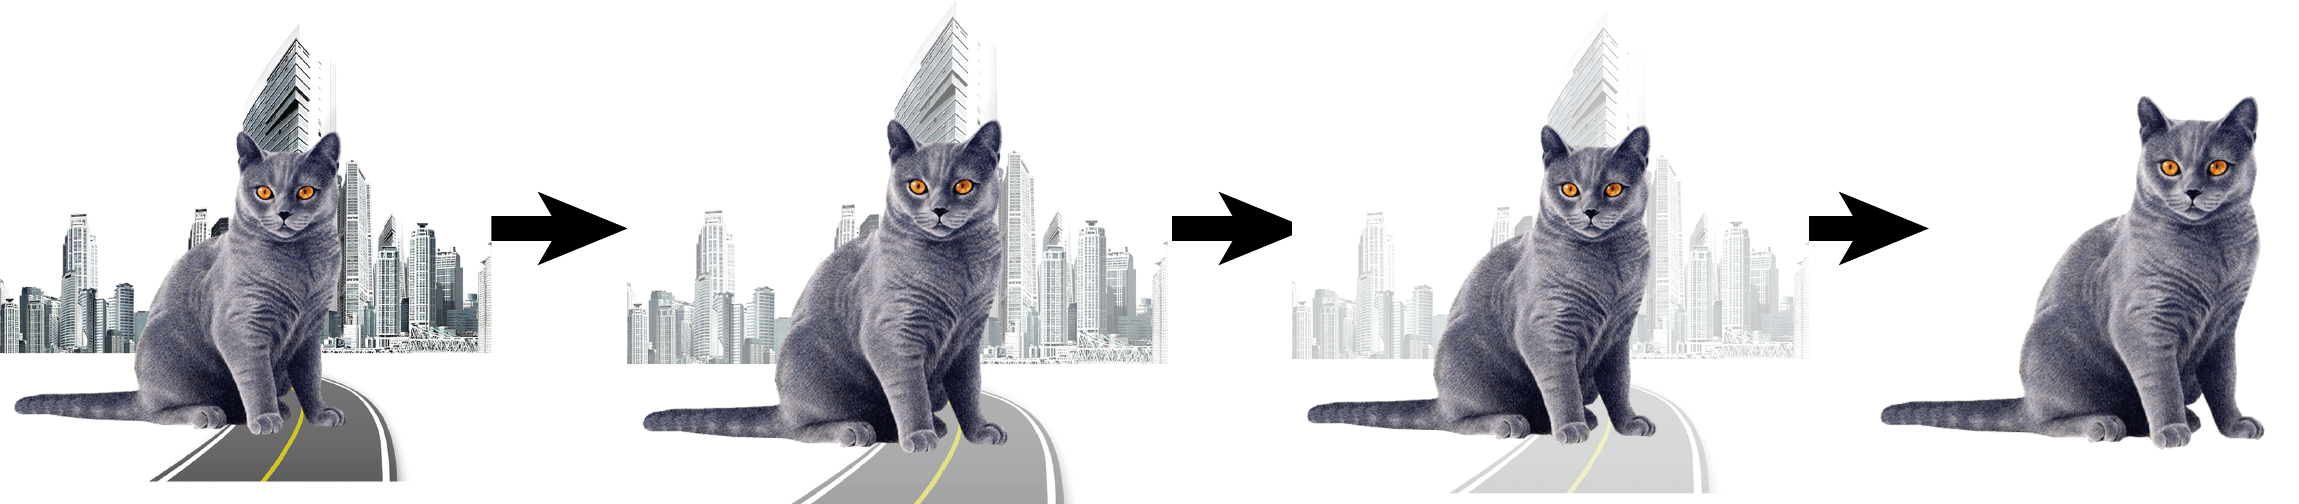
\includegraphics[width=\linewidth]{sections/1_adaptinit/imgs/info_2.png}
% \end{frame}



\begin{frame}{Tranable Scaling Factor}
	  An additional \textbf{scaling factor} \( \{a_{i} \in \mathbb{R} \text{ , }
  i = [0, \ldots, M]\}\) is introduced for each layer: 
  \begin{equation}
    \bm{y}_{i} = f_{i}(a_i, \bm{W}_i, \bm{b}_i;\bm{y}_{i-1}) =  g_{i}{(|a_{i}|\bm{W}_{i}\bm{y}_{i-1} + \bm{b}_i)} \in \mathbb{R}^{N_i},
  \end{equation}
  {\scriptsize where \(|\cdot|\) denotes the absolute value operator,
    \(g_{i}(\cdot): \mathbb{R}^{N_{i-1}} \rightarrow \mathbb{R}^{N_{i-1}}\), the
    activation functions, \(\bm{W}_i \in \mathbb{R}^{N_{i} \times N_{i-1}}\) and
    \(\bm{b}_i \in \mathbb{R}^{N_{i}}\) are the weights and biases of the layer,
    respectively.} 

    \begin{center}
        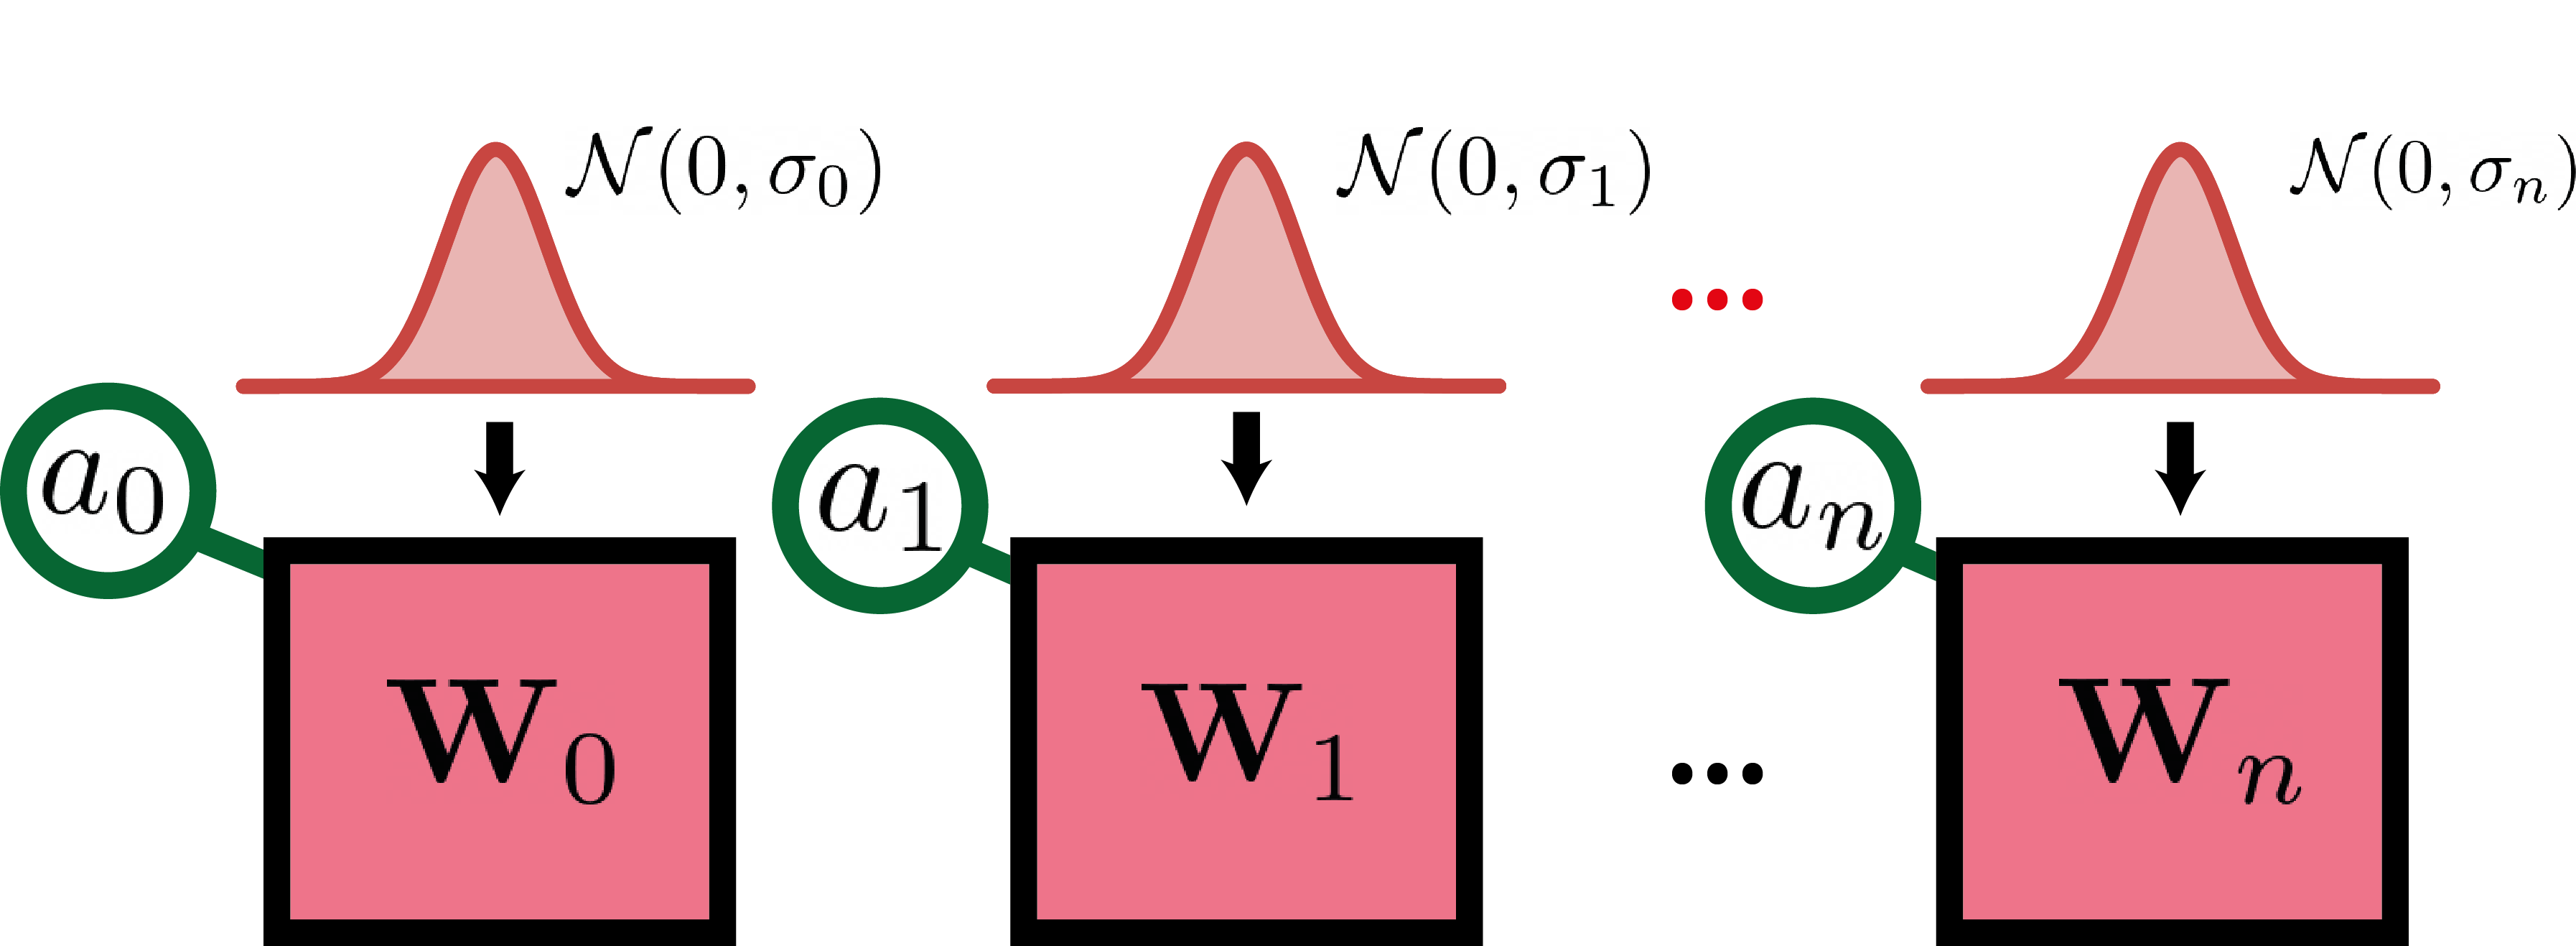
\includegraphics[width=\linewidth]{sections/1_adaptinit/imgs/adapt_init_2.png}
    \end{center}    
\end{frame}

\begin{frame}{Reparameterization Trick}

\textbf{Altering the value of \(a_i \in \mathbb{R}\)} is equivalent to \textbf{altering the initialization variance} of the corresponding layer, $\mathbf{W}_i \sim \mathcal{N}_{N_{i} \times N_{i-1}}\left(0, (\alpha_i \sigma_i)^2 \right)$.

    \begin{center}
        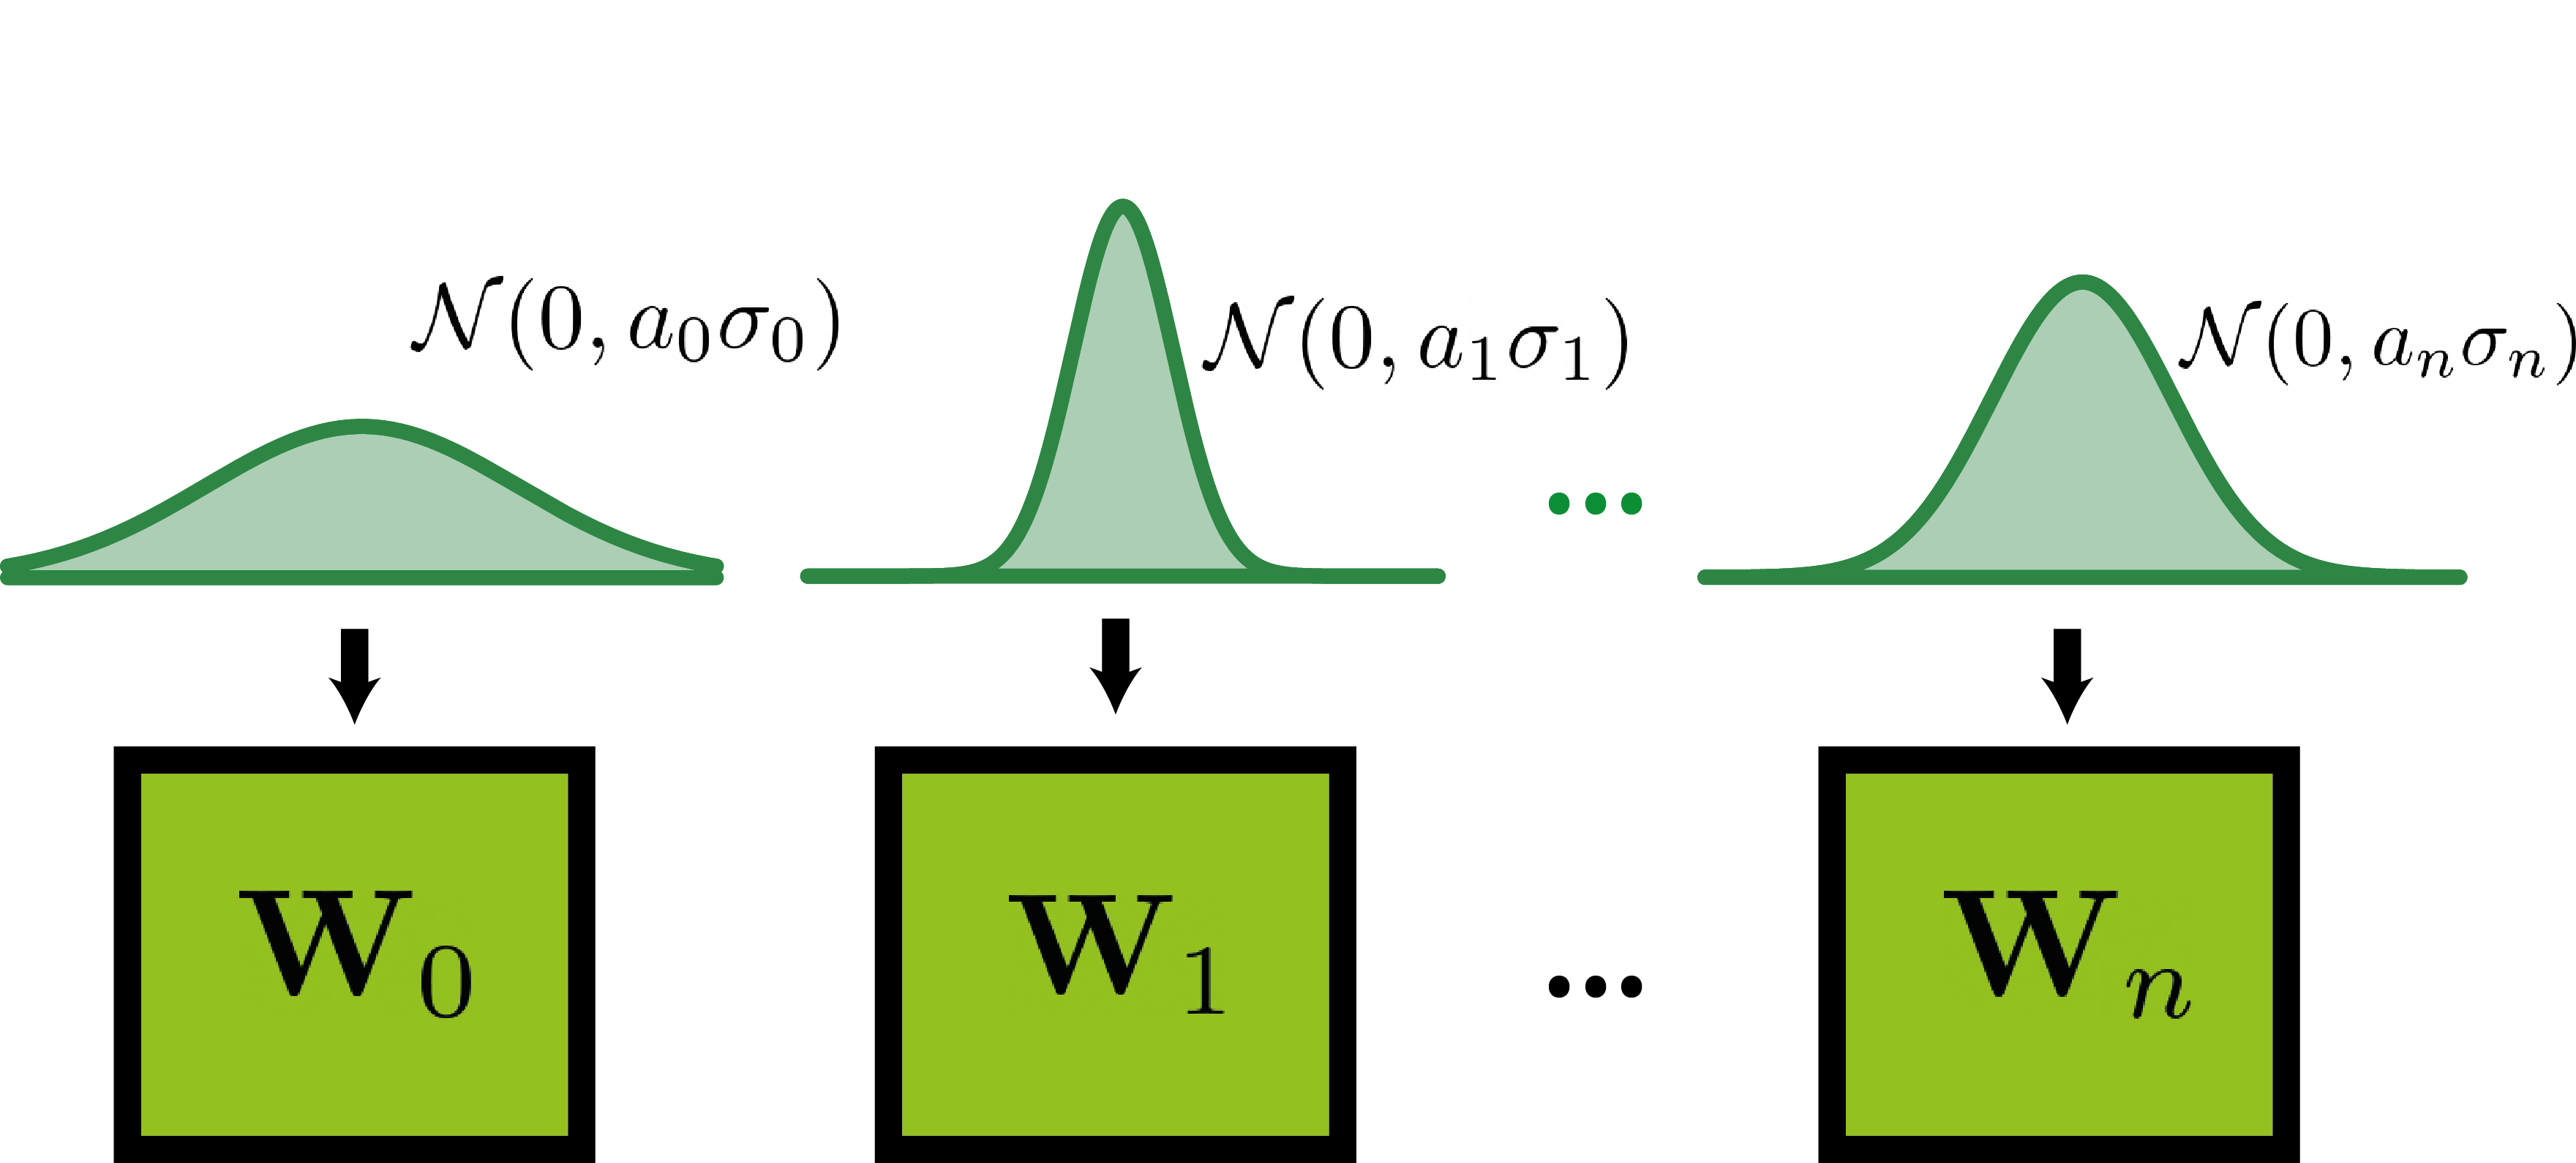
\includegraphics[width=\linewidth]{sections/1_adaptinit/imgs/adapt_init_3.png}    
    \end{center}
    
\end{frame}

% \begin{frame}
% 	Directly drawing values from a Gaussian distribution \(\mathcal{N}(\mu,
%   \sigma)\) that maximizes mutual information and initializing each layer's weights with them
%   would be the ideal scenario for an initialization scheme.
%   However, learning the parameters \(\mu \in \mathbb{R}\) and \(\sigma \in
%   \mathbb{R}\) directly is not 
%   possible, since the Gaussian distribution is not differentiable. What we propose
%   is to indirectly estimate them by fitting an estimator that we expect to work
%   best when the mutual information between the extracted representation and
%   the target variable is maximized. Moreover, estimating mutual information in
%   high-dimensional spaces is especially challenging and
%   inefficient.
% \end{frame}


% \begin{frame}
%   To this end, we can formulate an optimization problem based on the Data Processing Inequality to maximize the information for the \(k\)-th layer during the initialization:
% \begin{equation}
%     \begin{aligned}
%         \text{maximize } \quad &  I(Y_k, \hat{Y}), \text{ }  \forall k \in [0, M],\\
%         \text{s.t. } \quad &  \bm{W}_{k} \sim N(0,a_k\sigma^2), \\
%         & a_k > 0, \\
%     \end{aligned}
% \end{equation}
% {\scriptsize where \(M \in \mathbb{N}\) is the number of layers.}
% \end{frame}

\begin{frame}{Trainable Auxiliary Layer}
  % Since the Gaussian distribution is not differentiable and calculating the
  % information preserved for each layer is time consuming,
  % We propose to estimate the optimal variance for weight initialization
  % stochastically through an auxiliary classification task.

  The scaling  factor \(a_{i} \in \mathbb{R}\) is \textbf{progressively optimized} for
  each layer \textbf{through an auxiliary layer} 
    \begin{gather}
      \begin{split}
        \bm{y}_{k}^{class} & =  I_k^{adapt}(a_k, \bm{W}_k^{class}; \bm{x})\\
                          & = g^{class}(\bm{W}_k^{class}g_k(|a_k|\bm{W}_k
        f_{k-1}(\cdots(f_0(\bm{x})))) + \bm{b}_{k} \in \mathbb{R}^{N_c},
      \end{split}
    \end{gather}
{\scriptsize where \(\bm{x} \in \mathbb{R}^{N_0}\) is the input of the network and
\(\bm{W}_k^{class} \in \mathbb{R}^{N_c \times N_{k}}\).}

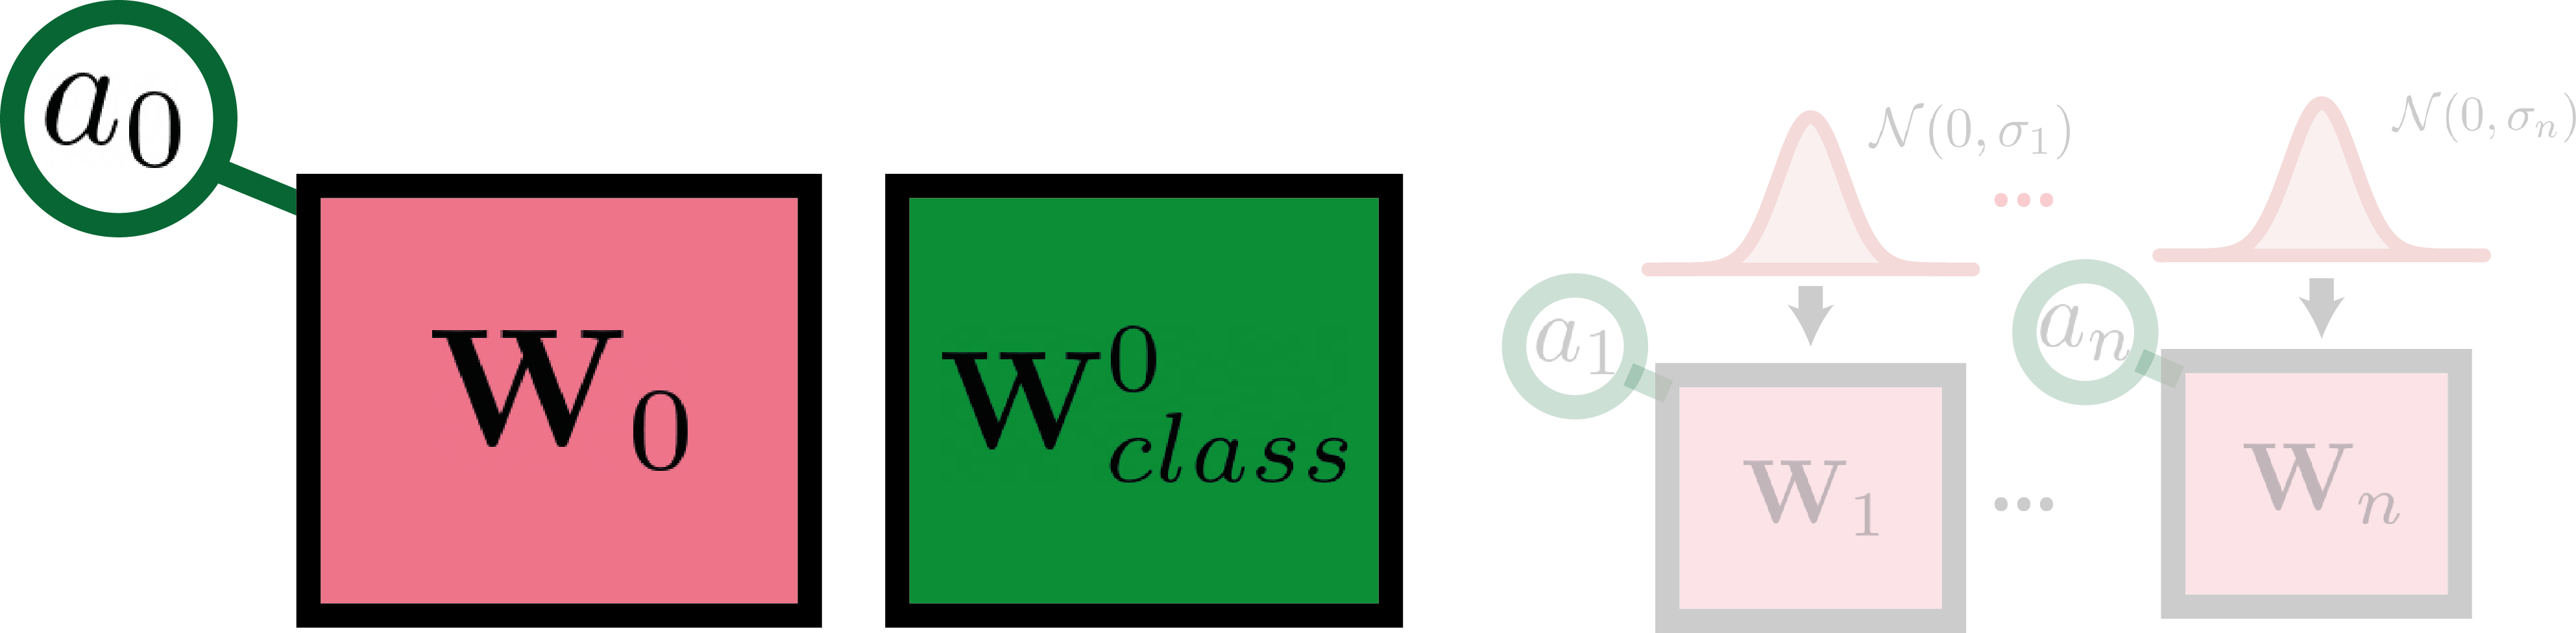
\includegraphics[width=\linewidth]{sections/1_adaptinit/imgs/adapt_init_4.png}
\end{frame}

% \begin{frame}{Regularization Term}
%   Since the proposed initialization targets to maximize the information
%   extracted from each layer, a regularization term is introduced to penalize
%   scaling factors that lead to saturated activation functions.
%   \begin{equation}
%     \tilde{J}(a_i, \bm{W}_i^{class}; \bm{x}, \bm{y}) = J(a_i, \bm{W}_i^{class}; \bm{x},
%     \bm{y}) + \gamma\Omega(\bm{z}_k) \in \mathbb{R},
%   \end{equation}
%   {\scriptsize where \(\gamma \in \mathbb{R}_+\) is the weighting factor for the penalty term.}

%   And \(\Omega(\cdot)\) is computed as:

% \end{frame}

% \begin{frame}{Optimization Process}
%   Finally, the scaling factor \(a_i \in \mathbb{R}_{+}\) and classification
%   weights \(\bm{W}_i^{class} \in \mathbb{R}^{M_{i} \times N_{c}}\) are optimized
%   using gradient descent: 
%   \begin{gather}
%     \Delta a_i = - \eta \frac{\partial \tilde{J}}{\partial a_i} - \gamma\frac{\partial
%     \Omega}{\partial a_i} \in \mathbb{R} \text{, } 
%   \Delta\bm{W}_i^{class} = - \eta \frac{\partial  \tilde{J}}{\partial\bm{W}_i^{class}} \in \mathbb{R}^{N_c \times N_k},
%   \end{gather}
%   {\scriptsize where \(\tilde{J}(\cdot)\) is the cost function used for network training,
%   \(\eta \in \mathbb{R}^{+}\) is the learning rate used, and \(c \in
%   \mathbb{R}^{+}\) is the weight of the relative contribution of the penalty
%   term, \(\Omega\).}

%   \begin{equation}
%     \Omega(\bm{z}_{k}) = \frac{\sum_{j=0}^{N_k}\max\{\lim_{x\to -\infty}g_k(x) - z_k, z_k - \lim_{x\to +\infty}g_k(x), 0\}}{N_{k-1} N_{k}} \in \mathbb{R},
%   \end{equation}
%   {\scriptsize where \(N_{i} \in \mathbb{N}\) and \(M_{i} \in \mathbb{N}\) is the fan-in and
%   fan-out respectively and \(\max\{\cdot\}\) denotes the maximum element in the
%   set.}
% \end{frame}

% \begin{frame}{Adaptive Initialization Pipeline}

% \vspace{15pt}

%     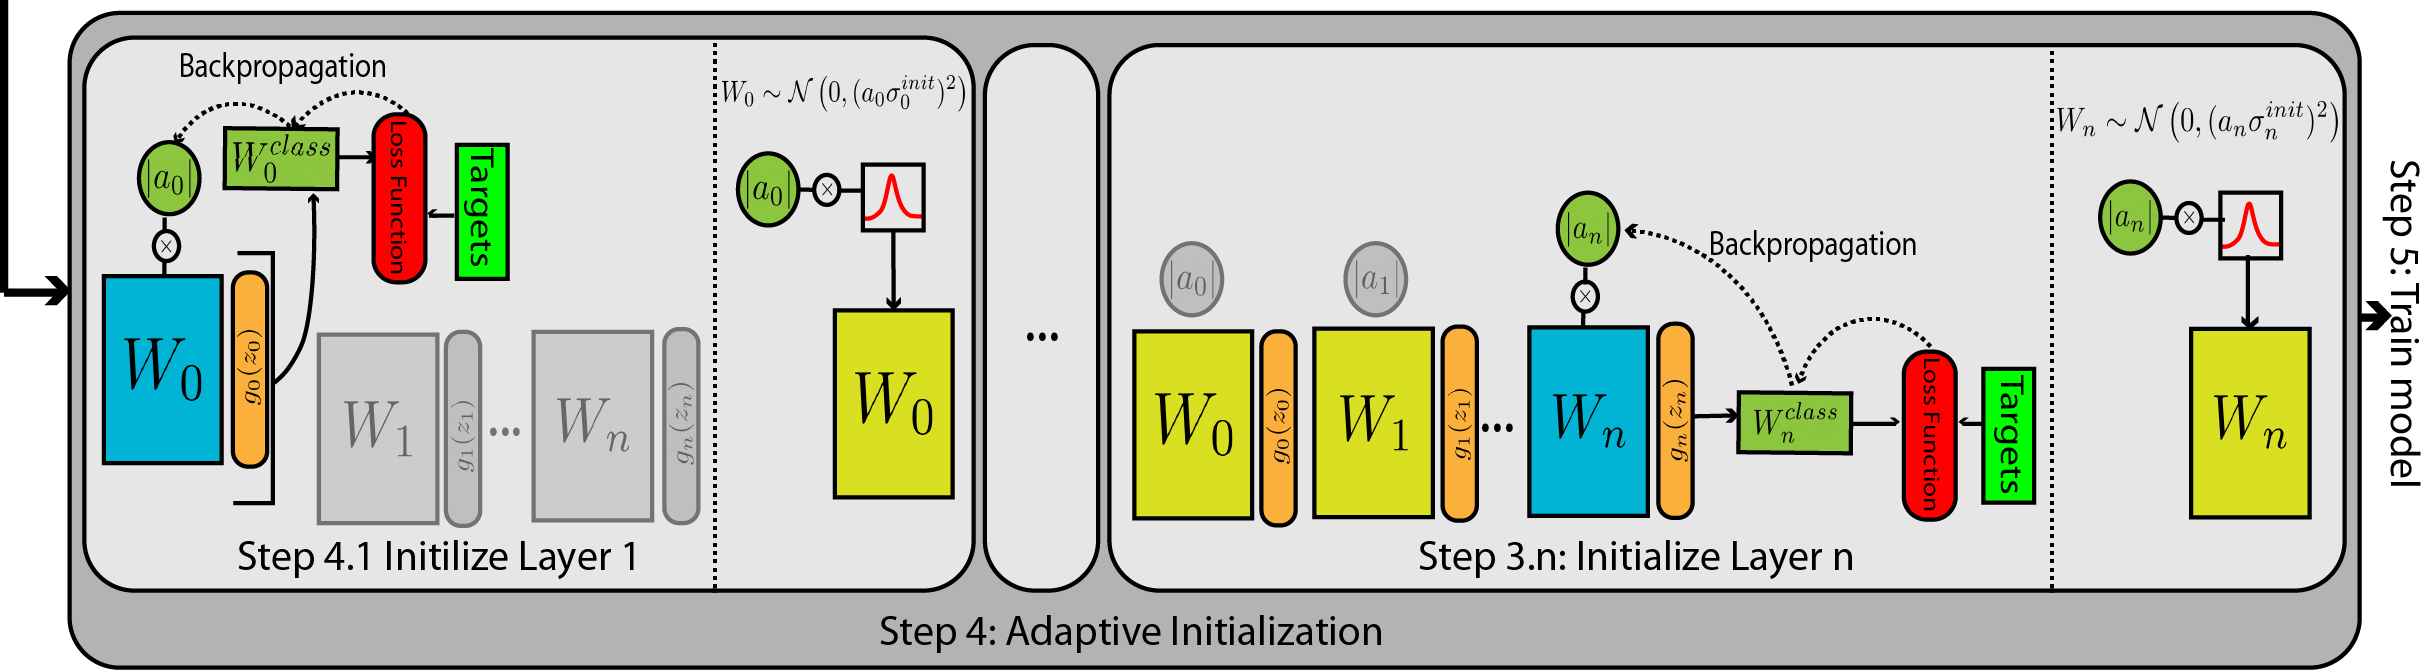
\includegraphics[width=\linewidth]{sections/1_adaptinit/imgs/adapt_init_5.png}


% \end{frame}


% \begin{frame}{Notes on proposed initialization}
% \begin{itemize}
%     \item The scale of the weights of the $i$-th layer are indirectly adapted
%       through $\alpha_i$ which is equivalent to initializing the layer with a
%       different variance.  
%     \item During the initialization process \textbf{none of the layers are
%         actually trained.} 
%     \item \textbf{The representations extracted from them are random
%         transformations/projections of the input data.} Such transformations
%       come with strong theoretical guarantees\footnote{Ali Rahimi et al. "Random
%         features for large-scale kernel machines." (NIPS'07)}. 
% \end{itemize}
% \end{frame}

\begin{frame}{Noise in Photonic Neuron}
\begin{center}
    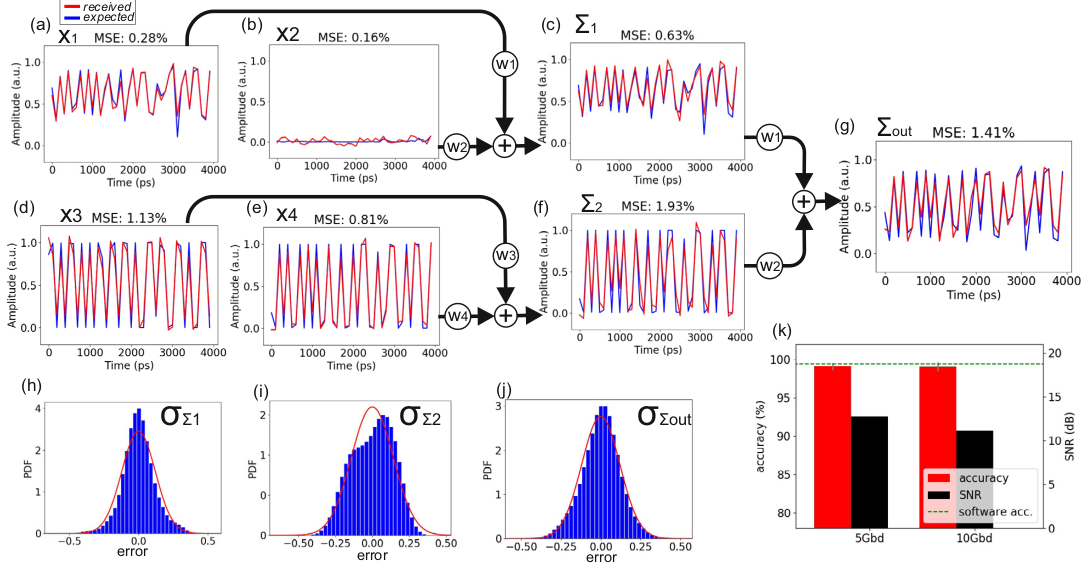
\includegraphics[width=0.9\linewidth]{sections/1_adaptinit/imgs/nature_no_noise.png}
\end{center} \vspace{-10pt}
  Different sources of noise can be \textbf{modeled} as a channel with an
   \textbf{Additive White Gaussian Noise (AWGN)}\footnote{\scriptsize Mourgias-Alexandris, G., Moralis-Pegios, M., Tsakyridis, A., Simos, S., Dabos, G., Totovic, A., Passalis, N., \textbf{Kirtas, M.}, Rutirawut, T., Gardes, F.Y. and Tefas, A., 2022.  \href{https://www.nature.com/articles/s41467-022-33259-z}{Noise-resilient and high-speed deep learning with coherent silicon photonics}. Nature communications, 13(1), p.5572} 
\end{frame}

\begin{frame}{Noise-aware Training}
  Exploiting the fact that \textbf{DL models are intrinsically resistant to noise},
  the proposed initialization treats noise as an intrinsic characteristic of the
  network.
  
    \begin{center}
        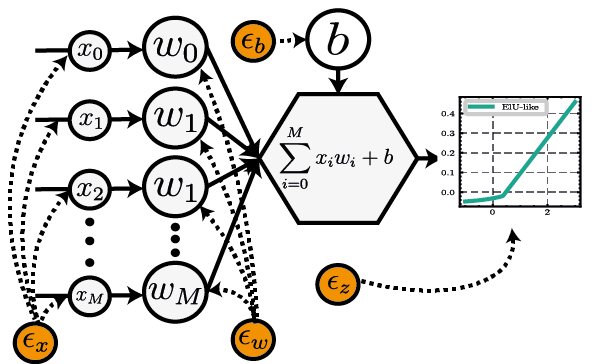
\includegraphics[width=0.6\linewidth]{sections/2_quant/imgs/quant_neuron.png}    
    \end{center}  
  \begin{equation*}
    z_{ij} =  {\sum_{j=1}^{N_k} \left( w_{ij} + \mathcal{N}(0, \sigma^2_w ) \right)}\left( x_{i-1,j} + \mathcal{N}(0, \sigma^2_x)\right) + \left(b_{i} + \mathcal{N}(0, \sigma^2_b)\right) \in \mathbb{R},
  \end{equation*}
  {\scriptsize where \(\sigma^2_x \in \mathbb{R}\), \(\sigma^2_w \in \mathbb{R}\) and  \(\sigma^2_b \in \mathbb{R}\) are the variances of the noise that
  affects the input, weighting, and bias mechanism, respectively.}
  
  % Thus, the basic noise sources and components of the DL system is
  % taken into account during training.
  % With the output of a noisy neuron modeled as:  
  
  %  And the final output of the neuron is modeled as:
  % \begin{equation}
  %   y_{ij} = g(u_{ij}) + \mathcal{N}(0, \sigma^2_g),
  % \end{equation}
  % {\scriptsize where \(\sigma^2_g\) is the variance of the noise induced by the activation
  % function.}
\end{frame}


% \begin{frame}{DL models - noise resistant}
%     Most of the existing works are \textbf{limited on evaluating the effect of
%       noise during the inference and after the network has already been
%       trained.} 
    
%     Overlooking the fact that DL models are \textbf{intrinsically resistant to
%       noise}, especially when they are first appropriately \textbf{trained to
%       withstand noisy signals.\footnote{N. Passalis, et al. , "Training Deep
%         Photonic Convolutional Neural Networks With Sinusoidal Activations,"
%         IEEE Transactions on Emerging Topics in Computational Intelligence,
%         (2019)}}\\ 
    
%     \vspace{0.5cm}
    
%     \textbf{\textcolor{mygreen}{A co-design approach can lead to significant
%         improvements.}} 
%       \end{frame}

\begin{frame}{Noise-aware Adaptive Initialization}
\begin{itemize}
    \item \textbf{After estimating the variance} for the first layer, the layer
      is appropriately re-initialized and \textbf{the weights
        $\mathbf{W}^{class}_i$ are discarded}.
    
    \item The initialization process \textbf{continues with the remaining layers.}

    \item \textbf{After all the layers have been initialized} using the proposed
       method, \textbf{the network is trained} in an end-to-end fashion. 
\end{itemize}

  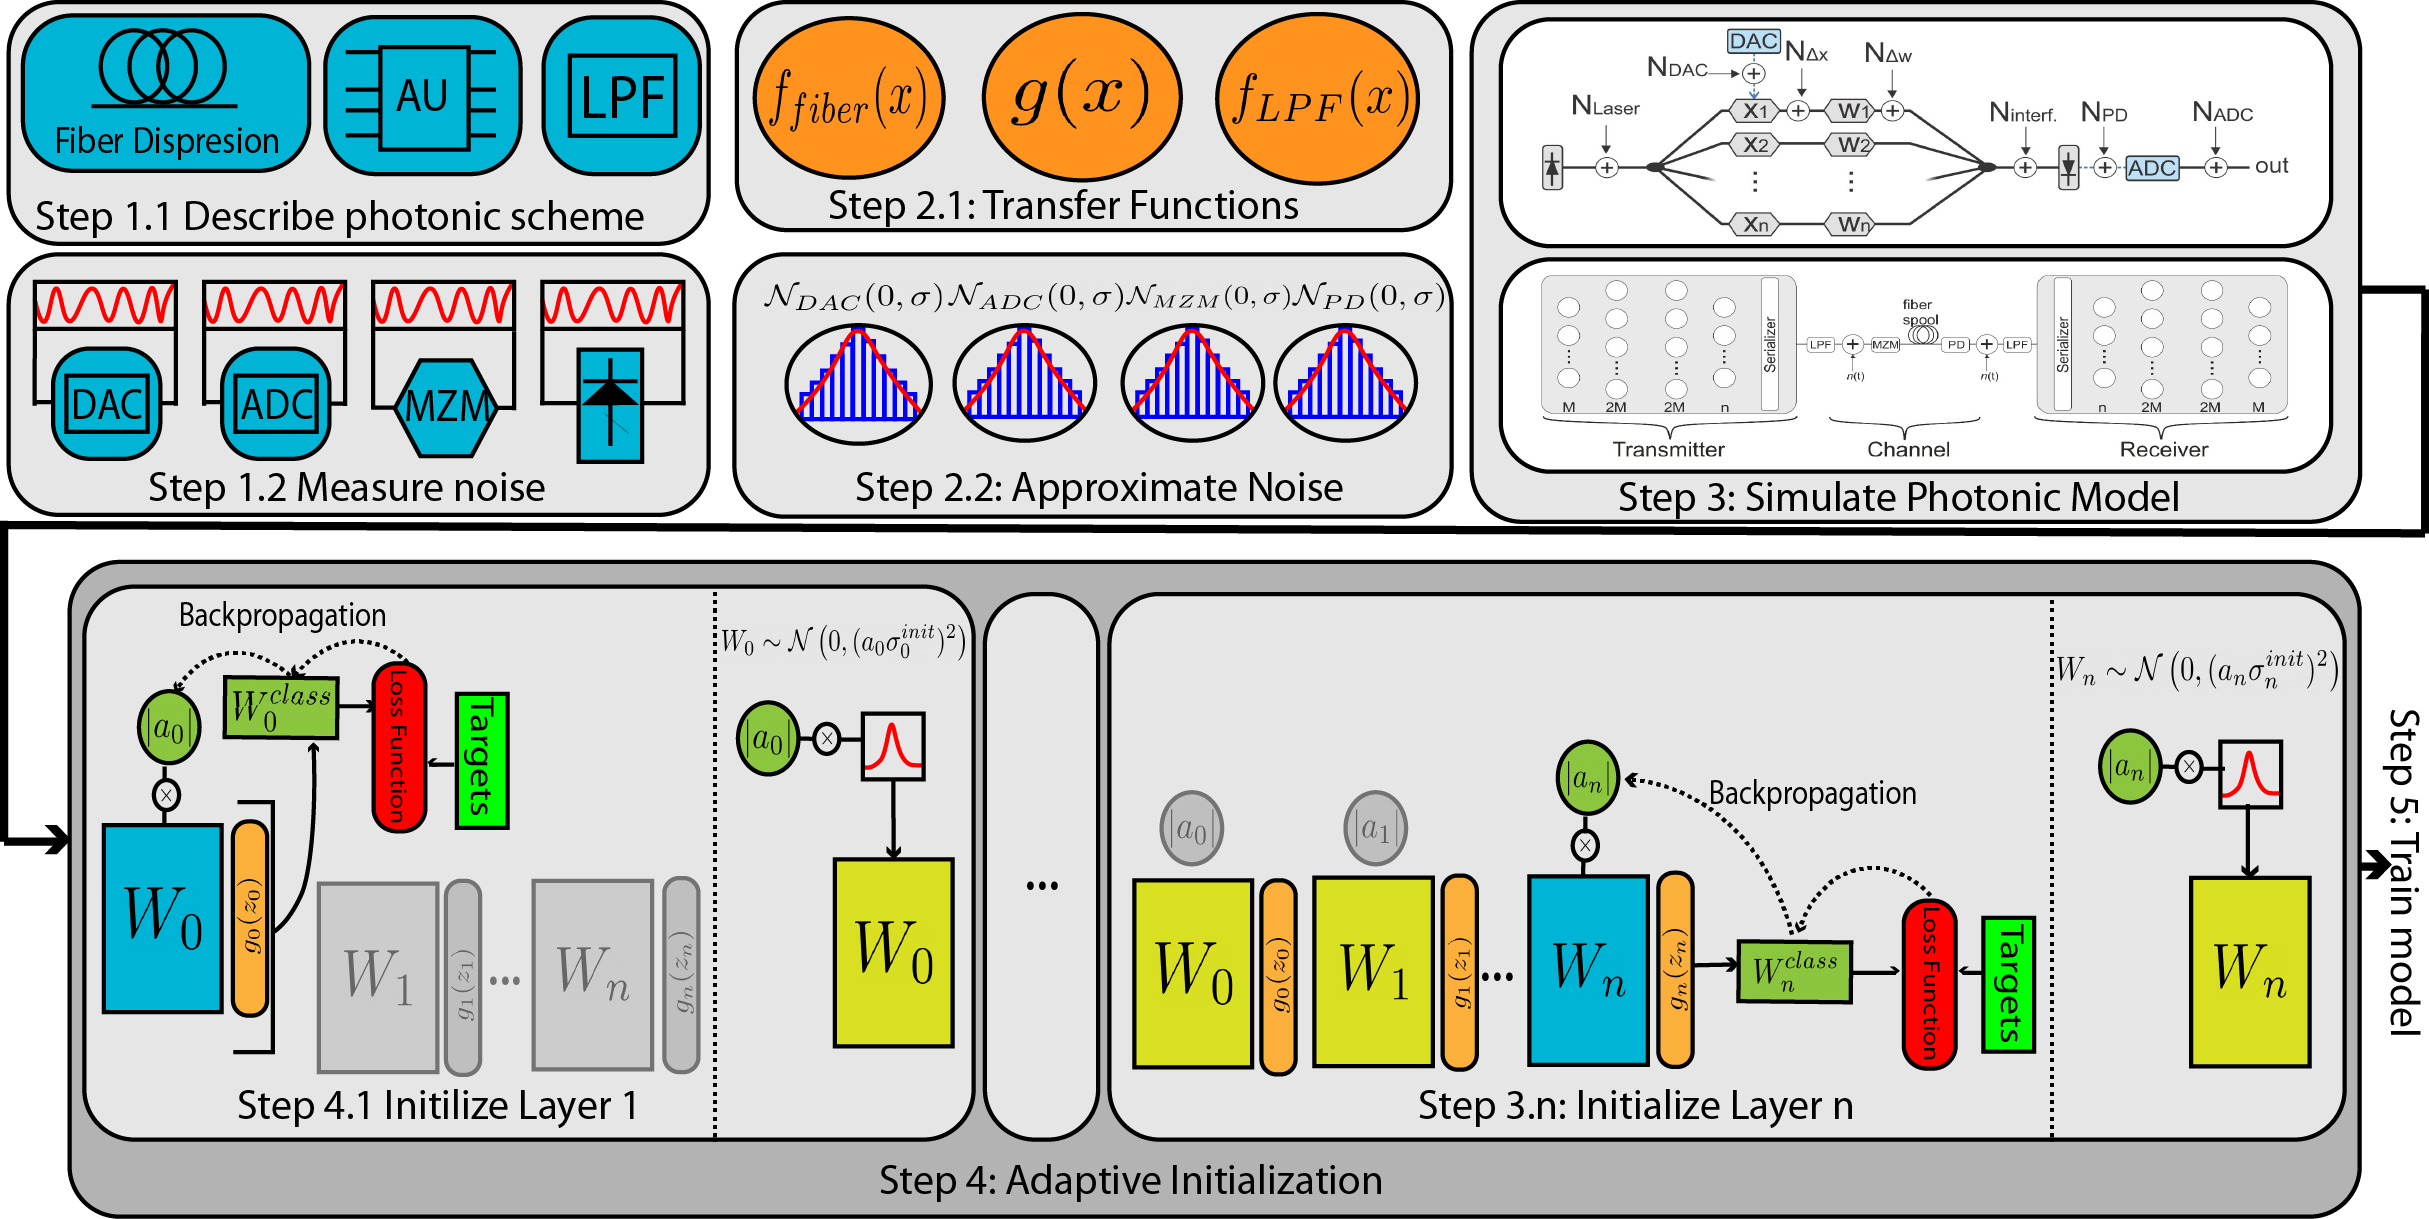
\includegraphics[width=\linewidth]{sections/1_adaptinit/imgs/Flow_diagram_new_latest.png}
\end{frame}

		
% \section{Experimental Evaluation}

% \section{Photonic Recurrent Networks}    
% \begin{frame}{FI-2010 Task}
% \begin{itemize}
%     \item For evaluating the proposed method, a challenging \textbf{large-scale high-frequency limit order book dataset (FI-2010)}\footnote{Paraskevi Nousi, et al., "Machine Learning for Forecasting Mid-Price Movements Using Limit Order Book Data" IEEE Access 7 (2019): 64722-64736} is employed. %~\cite{nousi2019machine}
%     \item The FI-2010 dataset contains more than \textbf{4 million limit orders collected from 5 Finnish companies.}
%     \item The forecasting task concerns the prediction of the \textbf{direction of the future mid-price movement} (up, down or stationary) after 10 time-steps.
% \end{itemize}
% \end{frame}

% \begin{frame}{Sigmoid-based recurrent photonic neurons}
%     The employed \textbf{recurrent photonic architecture} is composed of multiple recurrent photonic neurons. 
%     \begin{figure}  
%         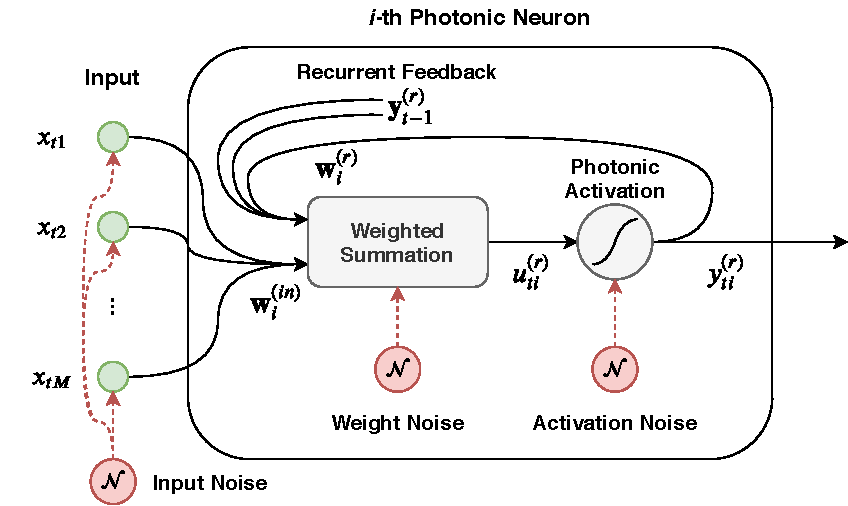
\includegraphics[scale=0.5]{sections/1_adaptinit/imgs/photonic_noisy.pdf}
%     \end{figure}
%      The final weighted output of the $i$-th recurrent neuron is then calculated as:
%     \begin{equation}
%     \label{eq:weighted-sum-rec}
%     u_{ti}^{(r)} = {\mathbf{w}_i^{(in)}}^T \mathbf{x}_{t} + {\mathbf{w}_i^{(r)}}^T \mathbf{y}^{(r)}_{t-1}.
%     \end{equation}
%     \begin{center}
%         \textit{  {\footnotesize Note that we omitted the bias term to simplify the employed notation.}}
%     \end{center}
% \end{frame}	

% \begin{frame}{Experimental Setup}
% \begin{itemize}
%     \item Photonic DL model for the conducted experiments is composed of:
%     \begin{itemize}
%         \item a recurrent photonic layer with 32 neuron
%         \item followed by two fully connected layers with 512 and 3 output respectively (same photonic architecture)
%     \end{itemize}
%     \item The length of the time series is 10
%     % \item Trained for 20 epochs with learning rate of \(\eta=10^{-4}\)
%     \item The scaling factor \(\alpha_i\):
%     \begin{itemize}
%         \item was estimated using 10 epochs with only 5 recurrent time steps
%         \item with learning rate 0.1 
%     \end{itemize}
%     % \item RMSprop optimization algorithm were used for both processes
%     \item The \(\kappa\) accuracy is used to measure the forecasting accuracy
% \end{itemize}

% \end{frame}



% \begin{frame}{FI2010 Dataset: Experimental Results}
%     \begin{table}
%     \label{table:eval}
%     \centering
%     \resizebox{0.85\linewidth}{!}{
%     \begin{tabular}{l|cccc}
%      $\sigma^2$  & Regular Training & Noisy Training & Adaptive Init. & Proposed  \\
%      \hline
%      \multicolumn{5}{c}{Weight Noise ($\sigma_w=\sigma, \sigma_{in}=\sigma_a=0$)}\\
%      \hline
%      .1 & 0.0807 & 0.1146 & 0.1498 & \textbf{0.1712} \\
%      .3 & 0.0486 & 0.1257 & 0.0809 & \textbf{0.1514} \\
%      .5 & 0.0138 & 0.1199 & 0.0096 & \textbf{0.1228} \\
%      \hline
%      \multicolumn{5}{c}{Activation Noise ($\sigma_a=\sigma, \sigma_{in}=\sigma_w=0$)}\\
%      \hline
%      .1 & 0.0884 & 0.1079 & 0.1693 & \textbf{0.1897} \\
%      .3 & 0.0681 & 0.1197 & 0.1410 & \textbf{0.1732} \\
%      .5 & 0.0267 & 0.1041 & 0.0674 & \textbf{0.1351} \\   
%     \hline
%      \multicolumn{5}{c}{Input noise ($\sigma_{in}=\sigma, \sigma_a=\sigma_w=0$)}\\
%      \hline
%     .1 & 0.0923 & 0.1102 & 0.1324 & \textbf{0.1626} \\
%     .3 & 0.0635 & 0.1128 & 0.0975 & \textbf{0.1632} \\
%     .5 & 0.0179 & 0.1003 & 0.0381 & \textbf{0.1068} \\
%     \hline
%       \multicolumn{5}{c}{Weight/Activation/Input Noise  ($\sigma_{in}=\sigma_a=\sigma_w=\sigma$)}\\
%      \midrule
%      .1 & 0.0627 & 0.1195 & 0.1351 & \textbf{0.1566} \\
%      .3 & 0.0274 & 0.1085 & 0.0552 & \textbf{0.1253} \\
%      .5 & 0.0058 & 0.0917 & 0.0078 & \textbf{0.1000} \\
%      \hline
%      \multicolumn{5}{c}{No noise  + Adaptive Initialization: 0.1738}\\
%     \end{tabular}}
%     \vspace{-1em}
%     \end{table}
% \end{frame}	

% \begin{frame}{Image Classification: Experimental Results}
%   \begin{table}
%   \centering
%   \resizebox{.83\linewidth}{!}{
%   \begin{tabular}{l|c|c|c|c||c|c|c|c}
%     & \multicolumn{4}{c||}{FashionMNIST}  &  \multicolumn{4}{c}{CIFAR10} \\
%     \midrule
%     & \multicolumn{8}{c}{\thead{Noise Level}} \\
%     \midrule
%     Initialization & 0.0 & 0.05 & 0.1 & 0.2 & 0.0 & 0.05 & 0.1 & 0.2 \\
%     \midrule
%     & \multicolumn{8}{c}{Photonic Sigmoid}\\
%     \midrule
%     Xavier & $ 17.88 $ &	$ 23.31 $  & $ 29.36  $ &  $ 89.57 $ & $ 90.0 $ & $ 89.77 $  & $ 89.9  $ &  $ 90.33 $\\
%     \textbf{+ Proposed}  &\bm{$ 8.63 $} &  \bm{$ 12.4 $} & \bm{$ 19.21 $} &  \bm{$ 25.16 $} &\bm{$ 20.52 $} &  \bm{$ 29.4 $} & \bm{$ 37.33 $} &  \bm{$ 56.01 $}\\
%     \midrule
%     He  & $ 19.17 $ & $ 23.45 $ & $ 28.29 $ & $ 29.23 $  & $ 74.17 $ & $ 89.54 $ & $ 90.14 $ & $ 90.0 $  \\
%     \textbf{+ Proposed}   & \bm{$ 9.06 $} & \bm{$ 12.81 $} & \bm{$ 21.53 $} & \bm{$ 26.73 $} & \bm{$ 25.18 $} & \bm{$ 28.23 $} & \bm{$ 39.94 $} & \bm{$ 89.82 $}\\
%     \midrule
%     & \multicolumn{8}{c}{Photonic Sinusoidal}\\
%     \midrule
%     Xavier & $ 8.04 $  & $ 9.4 $  &  $ 11.85 $ & $ 28.83 $ & $ 18.62 $  & $ 21.06 $  &  $ 28.2 $ & $ 74.23 $\\
%     + Proposed & \bm{$ 7.65 $} &  \bm{$ 8.82 $} & \bm{$ 10.48 $} &  \bm{$ 16.75 $} &\bm{$ 16.36 $} &  \bm{$ 19.47 $} & \bm{$ 24.97 $} &  \bm{$ 41.55 $}\\
%     \midrule
%     % \cdashline{2-7}
%     He  &  $  9.16 $ & $ 10.22 $ & $ 14.51 $ & $ 24.38 $ &  $ 52.28 $ & $ 43.92 $ & $ 56.3 $ & $ 90.3 $ \\
%     \textbf{+ Proposed}  & \bm{$ 8.62 $} & \bm{ $ 9.54 $} & \bm{$ 12.0 $} & \bm{$ 16.03 $} & \bm{$ 21.67 $} & \bm{ $ 21.74 $} & \bm{$ 28.47 $} & \bm{$ 48.85 $}\\
%     \midrule
%     & \multicolumn{8}{c}{Sigmoid}\\
%     \midrule
%     Xavier & $ 90.0 $  & $58.46$  & $89.65$ &  $90.08$ & $ 90.0 $  & $ 89.97 $  & $ 89.53 $ &  $ 90.03 $ \\
%     \textbf{+ Proposed}  &\bm{$ 8.74 $} &  \bm{$ 9.11 $} & \bm{$ 11.14 $} &  \bm{$ 15.29 $} &\bm{$ 20.54 $} &  \bm{$ 25.93 $} & \bm{$ 25.75 $} &  \bm{$ 35.64 $}\\ 
%     \midrule
%     He   & $ 13.67  $ & $ 14.09 $ & $ 15.42 $ &  $ 18.66 $ & $ 90.0  $ & $ 90.63 $ & $ 89.98 $ &  $ 90.43 $\\
%     \textbf{+ Proposed}   & \bm{$ 8.81 $} & \bm{$ 10.26 $} & \bm{$ 12.37 $} & \bm{$ 16.18 $} & \bm{$ 23.81 $} & \bm{$ 25.33 $} & \bm{$ 32.21 $} & \bm{$ 42.45 $}\\
%     \midrule
%     \bottomrule
%   \end{tabular}}
% \end{table}
% \end{frame}

% \section{Optical Fiber Communication}

% \begin{frame}{Experimental Setup}
%     \begin{itemize}
%         \item  Proposed method is employed on an intensity modulation/direct detection(IM/DD) system which is \textbf{trained in an end-to-end fashion as a single feed-forward ANN}
%         \item The system is composed of a \textbf{neural transmitter, a channel and a neural receiver.} 
%         \item The channel introduces a \textbf{non-linear transfer function with noise} due to the fiber dispersion.
%         \item \textbf{Goal} is to obtain the signal in receiver with the \textbf{minimum Bit Error Rate} (BER) after transmitting it through the noisy channel.
%     \end{itemize}
% \end{frame}

% \begin{frame}{Experimental Setup}
%     \begin{figure}
%         \centering
%         % \includegraphics[scale=0.3]{images/fiber_link.jpg}
%     \end{figure}
    
%     \begin{itemize}
%         \item the input of the transmitter model, which is a 6-bit symbol, is \textbf{encoded in a one-hot-vector of size 64}.
%         \item transmitter is a \textbf{fully connected 3-layer feed-forward ANN}.
%         \item receiver gets the deserialized output of the channel as an input of \(n\) symbols.
%         \textbf{Receiver} consists of \textbf{2-hidden layers and an output layer} with softmax activation function.
%         \item both a photonic \textbf{sigmoid-based} architecture, as well as a \textbf{sinusoidal-based} architecture are employed
%     \end{itemize}
% \end{frame}


\begin{frame}{Optical Fiber Communication: Setup}
\begin{center}
    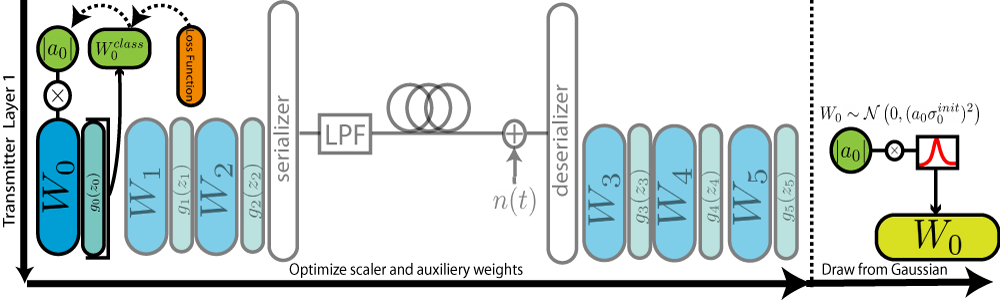
\includegraphics[width=\linewidth]{sections/1_adaptinit/imgs/pt1_flow.png}
    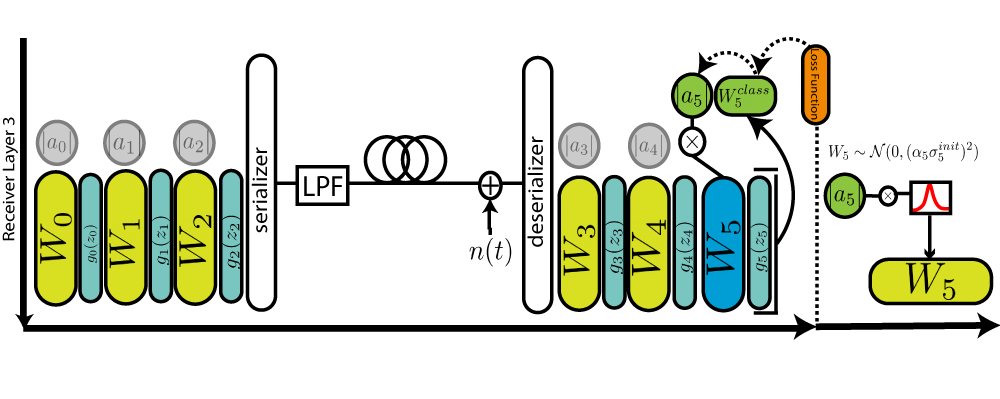
\includegraphics[width=\linewidth]{sections/1_adaptinit/imgs/pt2_flow.png}
\end{center}
\end{frame}


% \begin{frame}{Optical Fiber Communication:  Initialize Receiver}
%     \begin{figure}
%         \centering
%         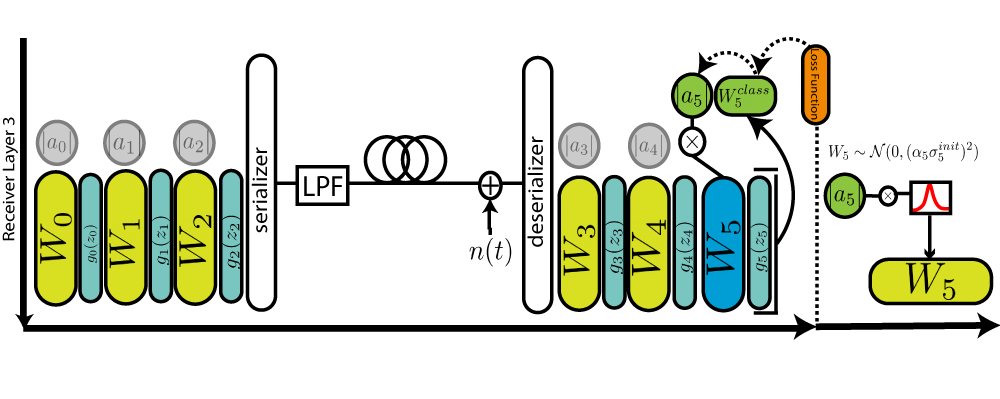
\includegraphics[width=\linewidth]{sections/1_adaptinit/imgs/pt2_flow.png}
%         \caption{Initialize third layer of receiver}
%         \label{fig:my_label}
%     \end{figure}
% \end{frame}


\begin{frame}{Optical Fiber Communication: Experimental Results}
\begin{table}
  \centering
  \resizebox{.83\linewidth}{!}{
  \begin{tabular}{p{0.5cm}|cc|cc}
  \(L\) & Xavier & + Proposed & He & + Proposed\\
     \hline
   & \multicolumn{4}{c}{Sigmoid} \\
    \hline
  30 & $ 7.38\times 10^{-3} $ & \bm{$ 5.65\times 10^{-5} $} & $ 9.90\times 10^{-4} $  & \bm{$ 8.20\times 10^{-5} $}\\
  40 & $ 5.15\times 10^{-3} $ & \bm{$ 3.41\times 10^{-3} $} & $ 3.26\times 10^{-3} $ & \bm{$ 3.68\times 10^{-4} $}\\
  50 & $ 1.11\times 10^{-2} $ & \bm{$ 4.79\times 10^{-3} $} & $ 5.30\times 10^{-3} $  & \bm{$ 1.39\times 10^{-3} $}\\
  60 & $ 7.38\times 10^{-3} $ & \bm{$ 3.06\times 10^{-3} $} & $ 7.66\times 10^{-3} $ & \bm{$ 2.77\times 10^{-3} $}\\
  70 & $ 6.94\times 10^{-3} $ & \bm{$ 5.85\times 10^{-3} $} & $ 6.76\times 10^{-3} $ & \bm{$ 5.42\times 10^{-3} $}\\
   \hline
   & \multicolumn{4}{c}{Photonic Sigmoid} \\
    \hline
  30 & $ 2.31\times 10^{-4} $ & \bm{$ 3.14\times 10^{-5} $} & $ 1.23\times 10^{-3} $ & \bm{$ 6.86\times 10^{-5} $}\\ 
  40 & $ 1.63\times 10^{-3} $ & \bm{$ 2.21\times 10^{-4} $} & $ 3.04\times 10^{-3} $ & \bm{$ 2.74\times 10^{-4} $}\\
  50 & $ 2.93\times 10^{-3} $ & \bm{$ 1.31\times 10^{-3} $} & $ 5.06\times 10^{-3} $ & \bm{$ 1.70\times 10^{-3} $}\\
  60 & $ 6.49\times 10^{-3} $ & \bm{$ 1.97\times 10^{-3} $} & $ 8.01\times 10^{-3} $ & \bm{$ 4.08\times 10^{-3} $}\\
  70 & $ 6.38\times 10^{-3} $ & \bm{$ 2.34\times 10^{-3} $} & $ 8.27\times 10^{-3} $ & \bm{$ 5.03\times 10^{-3} $}\\
  \hline
  & \multicolumn{4}{c}{Photonic Sinusoidal}\\
  \hline
    30 & $ 1.53\times 10^{-5} $ & \bm{$ 1.17\times 10^{-5} $} & $ 2.91\times 10^{-5} $ & \bm{$ 1.02\times 10^{-5} $}\\
  40 & $ 6.30\times 10^{-5} $ & \bm{$ 6.28\times 10^{-5} $} & $ 1.20\times 10^{-4} $ & \bm{$ 1.18\times 10^{-4} $}\\
  50 & $ 3.70\times 10^{-4} $ & \bm{$ 3.15\times 10^{-4} $} & $ 9.65\times 10^{-4} $ & \bm{$ 4.32\times 10^{-4} $}\\
  60 & $ 1.27\times 10^{-3} $ & \bm{$ 9.18\times 10^{-4} $} & $ 1.95\times 10^{-3} $ & \bm{$ 1.80\times 10^{-3} $}\\
  70 & $ 2.11\times 10^{-3} $ & \bm{$ 1.49\times 10^{-3} $} & $ 3.46\times 10^{-3} $ & \bm{$ 2.27\times 10^{-3} $}\\
    \hline
 \end{tabular}}
 \label{tab:eval-loss}
\end{table}
\end{frame}

\begin{frame}{Publications}
\begin{itemize}
    \item Main Journal Publications
    \begin{itemize}
        \item {\scriptsize \textbf{Kirtas, M.}, Passalis, N., Mourgias-Alexandris, G., Dabos, G.,
      Pleros, N. and Tefas, A., 2022. \href{https://ieeexplore.ieee.org/document/9815870}{Robust architecture-agnostic and noise resilient training of photonic deep learning models.} IEEE Transactions on Emerging Topics in Computational Intelligence.} 
    \end{itemize}
    \item Main Conference Publications 
        \begin{itemize}
        \item {\scriptsize \textbf{Kirtas, M.}, Passalis, N., Mourgias-Alexandris, G., Dabos, G., Pleros, N. and Tefas, A., 2022, August. \href{https://ieeexplore.ieee.org/abstract/document/9909781}{Learning photonic neural network initialization for noise-aware end-to-end fiber transmission.} In 2022 30th European signal processing conference (EUSIPCO)}
    \end{itemize}
    % \item Relevant Journal Publications
    %     \begin{itemize}
    %     \item 
    % \end{itemize}
    % \item Relevant Conference Publications
    %     \begin{itemize}
    %     \item {\scriptsize Passalis, N., \textbf{Kirtas, M.}, Mourgias-Alexandris, G., Dabos, G.,
    %   Pleros, N. and Tefas, A., 2021, January.\href{https://ieeexplore.ieee.org/abstract/document/9287649}{Training noise-resilient recurrent photonic networks for financial time series analysis.} In 2020 28th European Signal Processing Conference (EUSIPCO)}

    
\end{itemize}
\end{frame}



%   \begin{table}
%   \caption{FashionMNIST - Classification Error (\%)  for Different Activation Functions and Noise Levels}
%   \centering
%   \begin{tabular}{l|c|c|c|c||c|c|c|c}
%     & \multicolumn{4}{c||}{FashionMNIST}  &  \multicolumn{4}{c}{CIFAR10} \\
%     \midrule
%     & \multicolumn{8}{c}{\thead{Noise Level}} \\
%     \midrule
%     Initialization & 0.0 & 0.05 & 0.1 & 0.2 & 0.0 & 0.05 & 0.1 & 0.2 \\
%     \midrule
%     & \multicolumn{8}{c}{Sigmoid}\\
%     \midrule
%     Xavier & $ 90.0 $  & $ 89.97 $  & $ 89.53 $ &  $ 90.03 $ \\
%     &\bm{$ 20.54 $} &  \bm{$ 25.93 $} & \bm{$ 25.75 $} &  \bm{$ 35.64 $}\\ 
%     \midrule
%     He   & $ 90.0  $ & $ 90.63 $ & $ 89.98 $ &  $ 90.43 $\\
%     \textbf{+ Proposed}   & \bm{$ 23.81 $} & \bm{$ 25.33 $} & \bm{$ 32.21 $} & \bm{$ 42.45 $}\\
%     \midrule
%     & \multicolumn{8}{c}{Photonic Sigmoid}\\
%     \midrule
%     Xavier  & $ 90.0 $ & $ 89.77 $  & $ 89.9  $ &  $ 90.33 $\\
%     \textbf{+ Proposed}  &\bm{$ 20.52 $} &  \bm{$ 29.4 $} & \bm{$ 37.33 $} &  \bm{$ 56.01 $}\\
%     He  & $ 74.17 $ & $ 89.54 $ & $ 90.14 $ & $ 90.0 $  \\
%     \textbf{+ Proposed}   & \bm{$ 25.18 $} & \bm{$ 28.23 $} & \bm{$ 39.94 $} & \bm{$ 89.82 $}\\
%     \midrule
%     & \multicolumn{8}{c}{Photonic Sinusoidal}\\
%     \midrule
%     Xavier & $ 18.62 $  & $ 21.06 $  &  $ 28.2 $ & $ 74.23 $\\
%     + Proposed &\bm{$ 16.36 $} &  \bm{$ 19.47 $} & \bm{$ 24.97 $} &  \bm{$ 41.55 $}\\
%     \midrule
%     % \cdashline{2-7}
%     He  & $ 52.28 $ & $ 43.92 $ & $ 56.3 $ & $ 90.3 $ \\
%     \textbf{+ Proposed}  & \bm{$ 21.67 $} & \bm{ $ 21.74 $} & \bm{$ 28.47 $} & \bm{$ 48.85 $}\\
%     \bottomrule
%   \end{tabular}
%   \label{tab:1_fashion_mnist}
% \end{table}



% \begin{frame}
% 	To this end, we propose an auxiliary
%   task based on the expectations that mutual information increases when the
%   loss between the extracted representation and the target variable is minimized.
%   In this way, fitting an auxiliary classification (or regression) layer can be
%   used as a proxy approximator. The motivation behind the proposed approach is
%   that if \(I(\hat{X}_i; Y)\) is maintained, then a simple linear classifier would
%   be able to extract some useful information about \(Y\). Therefore, instead of
%   directly learning the distribution parameters to maximize \(I(\hat{X}_i; Y)\),
%   we can efficiently optimize the parameters to maximize the information that can
%   be extracted using a linear classifier. Apart from using an efficient proxy for
%   optimization, a re-parameterization approach is also employed, which allows us
%   to draw from the fixed distribution \(\mathcal{N}(0, 1)\) which in turn is
%   appropriately scaled and translated using trainable parameters by intercepting a
%   classification-based proxy instead of quantitatively measuring mutual
%   information. This allows for effectively learning the initialization variance
%   using regular back-propagation, since instead of back-propagating the gradients
%   through the (non-differential) Gaussian distribution, we employ a differentiable
%   scaling scheme over it.
% \end{frame}

% \section{Normalized Quantization-aware Training}



\begin{frame}{Quantization Error}
  Another significant bottleneck is the use of expensive \textbf{high-speed} and precision \textbf{analog-to-digital} and 
  \textbf{digital-to-analog} conversion modules\footnote{\scriptsize Tsakyridis, A., Moralis-Pegios, M., Giamougiannis, G., \textbf{Kirtas,
    M.}, Passalis, N., Tefas, A. and Pleros, N., 2024.
  \href{https://pubs.aip.org/aip/app/article/9/1/011102/3161086}{Photonic
  neural networks and optics-informed deep learning fundamentals.} APL
Photonics, 9(1).}.

\begin{center}
  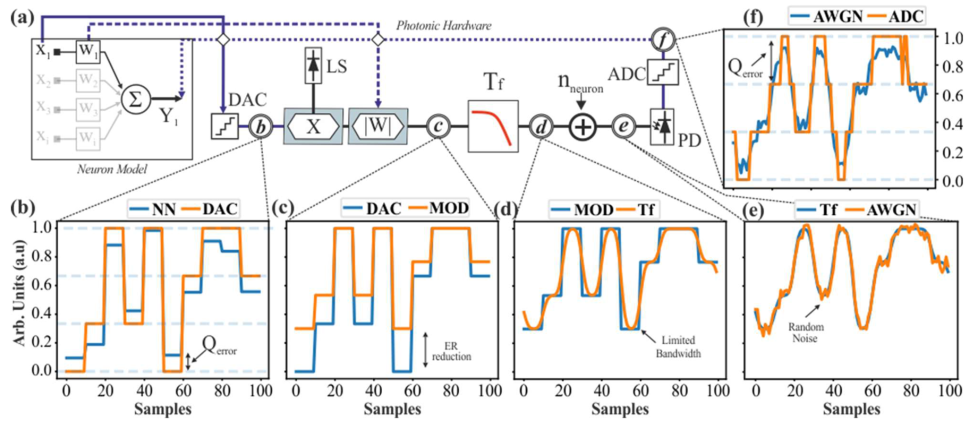
\includegraphics[width=0.8\linewidth]{sections/2_quant/imgs/apl_noise.png}  
\end{center}
  

  % This Chapter studies quantization phenomena in photonic models, induced by
  % DACs/ADCs, as an additional noise/uncertainty.

\end{frame}

% \begin{frame}{Contribution 2}
%   \textbf{(Contribution 2)}  A data driven quantization-aware training approach
%   that   
%   \begin{itemize}
%     \item Takes into account the distribution of parameters involved to the
%       decision of the networks
%     \item Eliminating the outliers
%       \item Reducing the quantization loss
%     \end{itemize}
%     Studied from the prospective of photonic hardware
%     \begin{itemize}
%       \item Taking into account DAC and ADC applied to the mechanism of neuron
%         (e.g. input, weight, activation)
%       \item Applying photonic-compliant uniform quantization to parameters
%       \end{itemize}
%      Allowing us to reduce the bit-resolution (< 8-bits) of DL models without significant
%      performance degradation.
% \end{frame}

%%%%%%%%%%%%%%%%%%%%%%%%%%%%%%%%%%%%%% NEW FRAME %%%%%%%%%%%%%%%%%%%%%%%%%%%%%%%%%%%%%%
\begin{frame}{Thesis contribution}
    \textbf{An activation-agnostic, quantization-aware training
      method}, oriented to PNNs. 
    \begin{itemize}
        \item \textcolor{mygreen}{Lower performance degradation when lower bit resolution applied} 
        \item \textcolor{mygreen}{Lower the hardware complexity and cost}
    \end{itemize}
    % Taking into account:
    % \begin{itemize}
    %     \item Quantization-errors occurred during training
    %     \item The distribution of parameters involved during training
    % \end{itemize}
    
    % \textbf{\textcolor{mygreen}{Motivated by the assumption that the weights
    %     involved in ANN inference follow a Gaussian distribution}} 
\end{frame}
%%%%%%% this assumption has 2 references, should we mention both or 1 is enough?
    
% \footnote{X. Glorot and Y. Bengio, “Understanding the difficulty of training
% deep feedforward neural networks,” in Proc. Int. Conf. on Artificial
% Intelligence and Statistics, 2010, pp. 249–256. 2, 3}


% %%%%%%%%%%%%%%%%%%%%%%%%%%%%%%%%%%%%%% NEW FRAME %%%%%%%%%%%%%%%%%%%%%%%%%%%%%%%%%%%%%%
% \begin{frame}{Quantization-aware Training}
%   Under the proposed quantization-aware training framework, \textbf{every signal
%     that is involved in the response of the \(i\)-th layer is first quantized in
%     a specific floating range} \([p^{(i)}_{min}, \dots ,p^{(i)}_{max}]\). 
% \begin{figure}
%   \centering
%     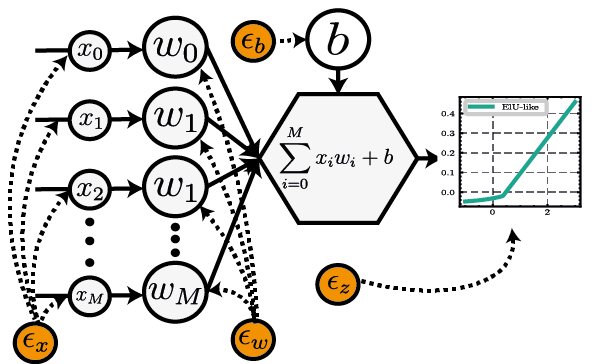
\includegraphics[width=0.65\linewidth]{sections/2_quant/imgs/quant_neuron.png}
% \end{figure}

% \textbf{During the evaluation, forward-pass quantization error \(\epsilon\) is injected by deploying the rounding of quantization arithmetically in floating point.}
% \end{frame}

% %%%%%%%%%%%%%%%%%%%%%%%%%%%%%%%%%%%%%% NEW FRAME %%%%%%%%%%%%%%%%%%%%%%%%%%%%%%%%%%%%%%
% \begin{frame}{Lower Bit Representation}
%   Under the proposed quantization-aware training framework, \textbf{every signal
%     that is involved in the response of the \(i\)-th layer is first quantized in
%     a specific floating range} \([p^{(i)}_{min}, \dots ,p^{(i)}_{max}]\) and they can be represented using \(B\) bits. 
    
%  First, \textbf{every signal} $p^{(i)}$ is \textbf{converted to a bit representation} by applying the function \( Q:\mathbb{R} \rightarrow \mathbb{N}\):
% \begin{equation}
%     p_{q}^{(i)} = Q(p^{(i)}, s_p^{(i)}, \zeta_p^{(i)}) =  clip \left\{\nint*{\frac{p^{(i)}}{s_p^{(i)}} + \zeta_{p}^{(i)}}, q_{min}, q_{max}\right\} \in \mathbb{N}
% \end{equation}
% {\scriptsize where \(p^{(i)} \in \mathbb{R}\), \(p_{q}^{(i)} \in [0\ldots, 2^B-1]\) and \(B\) denotes the bit resolution of the signal.}

% \textbf{Then, \(p_{q}^{(i)}\) is converted to discrete floating arithmetics} \(p_{q}^{(i)} \in [p^{(i)}_{min},  \ldots, p^{(i)}_{min}]\) using a dequantization function \(D: \mathbb{N} \rightarrow \mathbb{R}\):
% \begin{equation}
%     p_f^{(i)} = D(p^{(i)}_{q}, s_p^{(i)}, \zeta_p^{(i)}) = s_{p}^{(i)} (p_{q}^{(i)}-\zeta_{p}^{(i)}) \in \mathbb{R}
% \end{equation}

% \end{frame}

%%%%%%%%%%%%%%%%%%%%%%%%%%%%%%%%%%%%%% NEW FRAME %%%%%%%%%%%%%%%%%%%%%%%%%%%%%%%%%%%%%%
\begin{frame}{Quantization-aware Training}
The linear response of \(i\)-th layer is given by:
\begin{equation}
\bm{z}_{f}^{(i)} = Quant(\bm{W}_{f}^{(i)} \cdot \bm{y}_f^{(i-1)} + \bm{b}_f^{(i)}) \in \mathbb{R}^{N_i},
\end{equation}
{\scriptsize where \(Quant(\bm{x})\) denotes the process of quantization followed by dequantization of a vector or matrix \(\bm{x} \in \mathbb{R}^{M_i}\).}
\begin{center}
    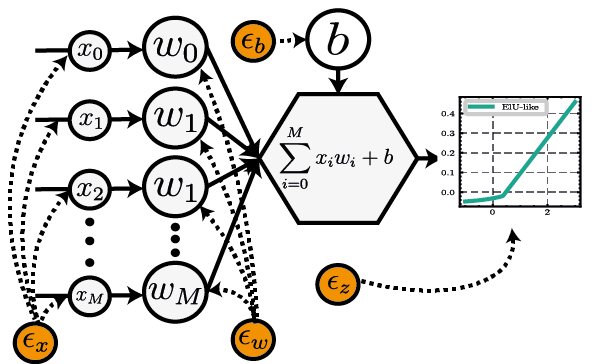
\includegraphics[width=0.6\linewidth]{sections/2_quant/imgs/quant_neuron.png}    
\end{center}
\begin{equation}
    \bm{y}^{(i-1)} = g^{(i)}((\bm{W}^{(i)} + \bm{\epsilon}_w) (\bm{y}^{(i-1)} + \bm{\epsilon}_y) + \bm{b}^{(i)} + \bm{\epsilon}_b) + \epsilon_g \in \mathbb{R}^{N_i}.
\end{equation}

% \textbf{The quantization error is propagated through the network} as a noise signal that is taken into account  \textbf{during training} affecting the overall performance of the network. 

% The output $\bm{z}_{f}^{(i)}$ passes through the photonic activation function, \(g(\cdot)\) of the neuron 
% \begin{equation}
%     \bm{y}^{(i)}_{f} = Quant(g( \bm{z}_{f}^{(i)})).
% \end{equation}
% \textbf{All signals involved in the layer's output are distributed in a uniform floating range between \(p_{min}^{(i)}\) and \(p_{max}^{(i)}\)} 
\end{frame}

% %%%%%%%%%%%%%%%%%%%%%%%%%%%%%%%%%%%%%% NEW FRAME %%%%%%%%%%%%%%%%%%%%%%%%%%%%%%%%%%%%%%
% \begin{frame}{Quantization-aware Training}


% % For example, for the weights $\bm{w}$, the quantization error is calculated as $\bm{\epsilon}_w = Quant(\mathbf{w}) - \mathbf{w}$.
% \end{frame}




%%%%%%%%%%%%%%%%%%%%%%%%%%%%%%%%%%%%%% NEW FRAME %%%%%%%%%%%%%%%%%%%%%%%%%%%%%%%%%%%%%%
\begin{frame}{Scaling Factor}
\tikzstyle{na} = [baseline=-.5ex]
\textbf{\textit{Scale}} defining the range of uniform bucket,
    \begin{equation}
        s^{(i)}_p= \frac{p^{(i)}_{max}-p^{(i)}_{min}}{q_{max}-q_{min}} \in \mathbb{R}^{+},
    \end{equation}
    {\scriptsize where \(q_{min}=0\) and \(q_{max} = 2^B-1\) denote the range of an \(B\)-bit resolution.}

    \begin{center}
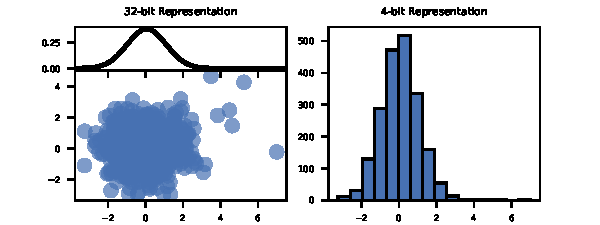
\includegraphics[\width=\linewidth]{sections/2_quant/imgs/motivation_1.pdf}    
\end{center}
\textbf{Effective range, i.e.,  minimum (\(p^{(i)}_{max} \in \mathbb{R}\)) and maximum (\(p^{(i)}_{min} \in \mathbb{R}\)) values} affects the amount of quantization error.

    % (0 and \(\) respectively) while \(p^{(i)}_{max} \in \mathbb{R}\) and \(\) represents the working range, i.e., maximum and minimum, of a signal.
    

% \textbf{Zero-point is a low precision value that represents the quantized value that will represent the real value 0}, and it is calculated as: 
% \begin{equation}
% \zeta_p^{(i)} = clip\left\{ \nint*{q_{min} - \frac{p^{(i)}_{min}}{s^{(i)}_p}} , q_{min}, q_{max}\right\} \in \mathbb{N}    
% \end{equation}

\end{frame}


% %%%%%%%%%%%%%%%%%%%%%%%%%%%%%%%%%%%%%% NEW FRAME %%%%%%%%%%%%%%%%%%%%%%%%%%%%%%%%%%%%%%
% \begin{frame}{Working Range}
%  \vspace{5pt}
%  % in inference, \textbf{is the selected working range, i.e.,  minimum (\(p_{min}\)) and maximum (\(p_{max}\)) values}, of a signal on which the scale of uniform buckets depends. 
% \end{frame}

% %%%%%%%%%%%%%%%%%%%%%%%%%%%%%%%%%%%%%% NEW FRAME %%%%%%%%%%%%%%%%%%%%%%%%%%%%%%%%%%%%%%
% \begin{frame}{Normalized Quantization}
% %  Assuming that every signal involved in the response of each
% % neuron follows a \textbf{Gaussian distribution,  i.e.,  \(p \sim \mathcal{N}(\mu, \sigma)\):}


% \textbf{The proposed method is more robust to outliers}
% \end{frame}

\begin{frame}{Normalized Quantization}
    Quantization is applied using the \textit{proxy} minimum and maximum.
\begin{gather}
\label{eq:proposed_statistics}
    p_{min} = \tilde{\mu}^{p}_{K} - \alpha\tilde{\sigma}^{p}_{K} \in \mathbb{R},  \text{   }
    p_{max} = \tilde{\mu}^{p}_{K} + \alpha\tilde{\sigma}^{p}_{K} \in \mathbb{R}.
\end{gather}


% {\scriptsize where \textbf{$\alpha$}  denotes the scaling factor that
% controls the coverage used of the estimated normal distribution.}
\begin{center}
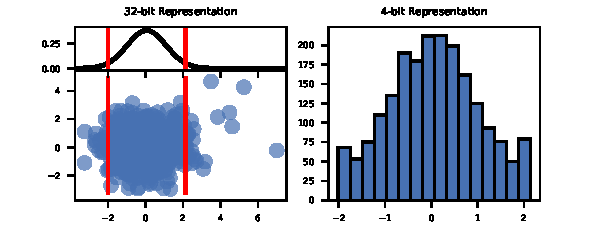
\includegraphics[\width=\linewidth]{sections/2_quant/imgs/motivation_2.pdf}    
\end{center}
Scaling factor $\alpha \in \mathbb{R}$ adjusts the coverage of the density area of the distribution according to the applied bit resolution.

Quantized parameters range \([\mu - \alpha\sigma^2, \ldots, \mu+\alpha\sigma^2] \in \mathbb{R}^N\) maintaining the \textbf{ maximum information at distribution's high density area}.
\end{frame}

% %%%%%%%%%%%%%%%%%%%%%%%%%%%%%%%%%%%%%% NEW FRAME %%%%%%%%%%%%%%%%%%%%%%%%%%%%%%%%%%%%%%
% \begin{frame}{Normalized Quantization Post training parameters}
% \begin{itemize}
%     \item 
% The probability of a normal deviation lies in the range \([\mu - \alpha\sigma, \mu + \alpha\sigma]\), based on the 68–95–99.7 rule, given by:
% \end{itemize}
% \begin{equation}
%      F(\mu +\alpha\sigma )-F(\mu -\alpha\sigma )= erf\left({\frac {\alpha}{\sqrt {2}}}\right) \in \mathbb{R},
% \end{equation}
% where \(F(\cdot)\) is the general form of the probability density function and \(erf(x)=\frac{2}{\sqrt{\pi}}\int_0^x e^{t^2}dt \) denotes the Gauss error function.
% \end{frame}

%%%%%%%%%%%%%%%%%%%%%%%%%%%%%%%%%%%%%% NEW FRAME %%%%%%%%%%%%%%%%%%%%%%%%%%%%%%%%%%%%%%
\begin{frame}{Estimated Parameters Distribution}
    Since the distribution of parameters is transformed during the training, the proposed method \textbf{progressively estimates} the distribution in every epoch by \textbf{applying an exponential moving average}.
\begin{gather}
    \label{eq:proposed_collection}
    \tilde{\mu}^{p}_{t} = \beta  E[\bm{p}_t] + (1 - \beta) \tilde{\mu}^{p}_{t-1} \in \mathbb{R}, \\
    \tilde{\sigma}^{p}_{t} = \beta Var[\bm{p}_t]^{1/2} + (1 - \beta) \tilde{\sigma}^{p}_{t-1} \in \mathbb{R},
\end{gather}
{\scriptsize where \(t = 1 \ldots K\), \(K \in \mathbb{N}\) denotes the number of epochs, and $\beta \in \mathbb{R}$ is a weighting parameter of the exponential average.}

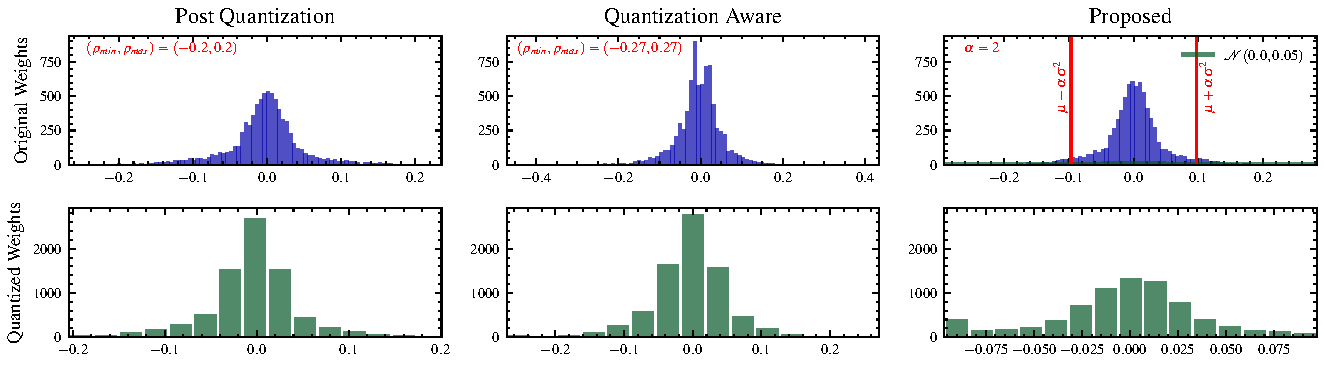
\includegraphics[width=\linewidth ]{sections/2_quant/imgs/mnist_histograms_layer_00.pdf}

\end{frame}



%%%%%%%%%%%%%%%%%%%%%%%%%%%%%%%%%%%%%% NEW FRAME %%%%%%%%%%%%%%%%%%%%%%%%%%%%%%%%%%%%%%
\begin{frame}{Quantization-aware \& Post Training Quantization}
\begin{center}
    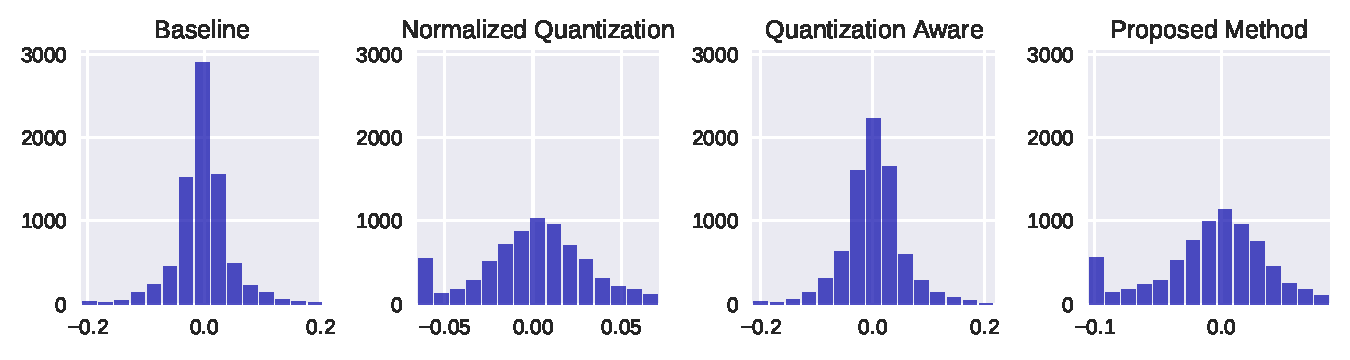
\includegraphics[width=\linewidth]{sections/2_quant/imgs/mnist_histograms_layer_0.pdf}
\end{center}

\textbf{Normalized-quantization can be used both in post training and quantization-aware training.}
\end{frame}

\begin{frame}{The Role of Coverage}
    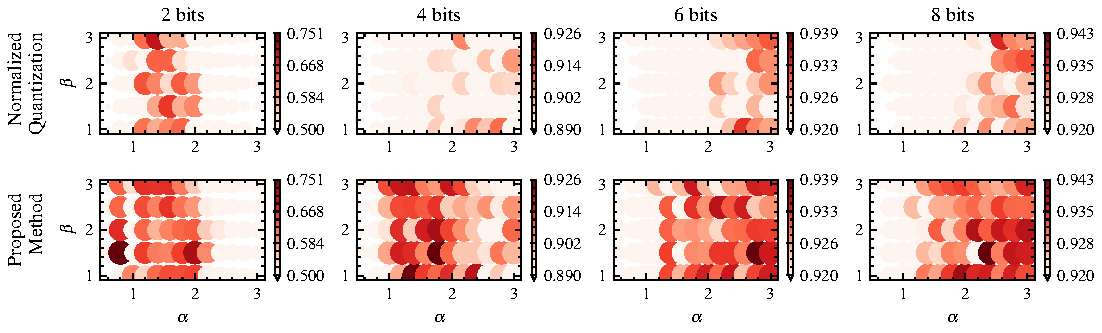
\includegraphics[width=\linewidth]{sections/2_quant/imgs/mnist_alpha_beta_plt.pdf}
    \begin{itemize}
        \item Intensity represents higher accuracy
        \item The normalized quantization do not highly depends on weighting parameter of the exponential average
        \item Tuning of scaling factor $\alpha \in \mathbb{R}$ should consider the applied bit resolution 
    \end{itemize}
\end{frame}



% \begin{frame}{Image Classification using FCNN}
% \begin{table}[h]
% \caption{Evaluating the proposed method on the MNIST dataset using a fully connected architecture (classification accuracy (\%) is reported).}
% \label{table:eval_mnist}
% \centering
% \resizebox{\linewidth}{!}{
% \begin{tabular}{l|cccc}
%     \toprule
%       \textbf{Bits} &  \textbf{Post Quant.} & \textbf{Norm. Post Quant.} & \textbf{Quant-aware Training} & \textbf{Proposed} \\
%      \midrule
%      \multicolumn{5}{c}{\textbf{Photonic Sinusoidal}}\\
%      \midrule
%      8 & $90.12 \pm{1.52}$ & $91.46 \pm 0.22$ & $91.21 \pm{0.49}$ & $\textbf{91.65} \pm \textbf{0.12}$\\
%      6 & $86.93 \pm{1.47}$ & $91.15 \pm 0.71$ & $91.04 \pm{0.51}$ & $\textbf{91.67} \pm \textbf{0.49}$\\
%      4 & $0.09 \pm{0.46}$ & $87.28 \pm 0.84$ & $90.26 \pm{0.77}$ & $\textbf{90.68} \pm \textbf{1.41}$\\
%      2 &  $0.09 \pm{0.26}$ & $66.36 \pm 4.53$ & $67.63 \pm{2.28}$ & $\textbf{79.31} \pm \textbf{2.06}$ \\
%      \midrule
%      \multicolumn{5}{c}{\textbf{Photonic Sigmoid}}\\
%      \midrule
%       8 & $91.02 \pm{0.81}$ & $91.81 \pm 0.36$ & $91.17 \pm{0.33}$ & $\textbf{91.79} \pm \textbf{0.25}$ \\
%       6 & $87.01 \pm{0.12}$ & $91.79 \pm 0.61$ & $91.02 \pm{0.29}$ & $\textbf{91.31} \pm \textbf{0.55}$ \\
%       4 & $0.09 \pm{0.25}$ & $87.14 \pm 0.21$ & $90.22 \pm{0.39}$ & $\textbf{90.76} \pm \textbf{0.37}$ \\
%       2 & $0.09 \pm{0.23}$ & $64.22 \pm 0.47$ & $61.26 \pm{1.95}$ & $\textbf{75.04} \pm \textbf{3.56}$\\
%      \bottomrule
% \end{tabular}}
% \label{tab:mnist_exp}
% \end{table}
% \end{frame}

%\subsection*{Image Classification using CNN}
\begin{frame}{Image Classification using CNNs}
\begin{table}[h]
\caption{Evaluating the proposed method on the CIFAR10 dataset using a convolutional architecture (classification accuracy (\%) is reported).}
\label{table:eval_cifar10}
\centering
\resizebox{\linewidth}{!}{
\begin{tabular}{l|cccc}
    \toprule
         \textbf{Bits} &  \textbf{Post Quant.} & \textbf{Norm. Post Quant.} & \textbf{Quant-aware Training} & \textbf{Proposed} \\
     \midrule
     \multicolumn{5}{c}{\textbf{Photonic Sinusoidal}}\\
     \midrule
     8 & $15.22 \pm{1.15}$ & $68.22 \pm 1.58$ & $67.64 \pm{1.24}$ & $\textbf{80.08} \pm \textbf{0.63}$\\
     6 & $15.10 \pm{1.81}$ & $63.61 \pm 0.79$ & $66.56 \pm{1.38}$ & $\textbf{77.81} \pm \textbf{0.43}$\\
     4 & $16.62 \pm{2.44}$ & $60.89 \pm 5.84$ & $29.48 \pm{10.43}$ & $\textbf{76.77} \pm \textbf{0.58}$\\
    %  2 &  $ \pm{}$ & $ \pm{} $ & $ \pm{}$ & $\textbf{} \pm \textbf{}$ \\
     \midrule
     \multicolumn{5}{c}{\textbf{Photonic Sigmoid}}\\
     \midrule
      8 & $16.39\pm{1.15}$ & $55.22 \pm 3.07$ & $66.23 \pm{1.23}$ & $\textbf{72.36} \pm \textbf{0.71}$ \\
      6 & $15.76 \pm{0.73}$ & $54.62 \pm 2.39$ & $66.56 \pm{1.61}$ & $\textbf{72.22} \pm \textbf{1.29}$ \\
      4 & $16.38 \pm{0.25}$ & $44.21 \pm 6.44$ & $65.25 \pm{1.96}$ & $\textbf{71.56} \pm \textbf{0.58}$ \\
    %   2 & $ \pm{}$ & $ \pm $ & $ \pm{}$ & $\textbf{} \pm \textbf{}$\\
     \bottomrule
\end{tabular}}
\label{table:3}
\end{table}
\end{frame}


%\subsection*{Image Classification using CNN}

% \textbf{\begin{frame}{Focasting using RNN}
%   \begin{table}
%     \caption{Evaluating the proposed method on the FI-2010 dataset using a recurrent architecture (Cohen's $\kappa$  is reported).}
%     \label{table:eval_fi2020}
%     \centering
%     \resizebox{\linewidth}{!}{
%       \begin{tabular}{l|cccc}
%         \toprule
%         \textbf{Bits} &  \textbf{Post Quant.} & \textbf{Norm. Post Quant.} & \textbf{Quant-aware Training} & \textbf{Proposed} \\
%         \midrule
%         \multicolumn{5}{c}{\textbf{Photonic Sinusoidal}}\\
%         \midrule
%         8 & $0.0502 \pm{0.0218}$ & $0.0840 \pm 0.0067$ & $0.1189 \pm{0.0105}$ & $\textbf{0.1347} \pm \textbf{0.0074}$\\
%         6 & $0.0647 \pm{0.0015}$ & $0.0825 \pm 0.0074$ & $0.1170 \pm{0.0115}$ & $\textbf{0.1342} \pm \textbf{0.0055}$\\
%         4 & $0.0645 \pm{0.0057}$ & $0.0756 \pm 0.0109$ & $0.1091 \pm{0.0210}$ & $\textbf{0.1184} \pm \textbf{0.0043}$\\
%         2 & $0.0370 \pm{0.0069}$ & $0.0416 \pm 0.0113$ & $0.0601 \pm{0.0031}$ & $\textbf{0.0782} \pm \textbf{0.0113}$\\
%         \midrule
%         \multicolumn{5}{c}{\textbf{Photonic Sigmoid}}\\
%         \midrule
%         8 & $0.0653 \pm{0.0081}$ & $0.0912 \pm 0.0085$ & $0.1262 \pm{0.0072}$ & $\textbf{0.1321} \pm \textbf{0.0024}$\\
%         6 & $0.0656 \pm{0.0061}$ & $0.0842 \pm 0.0042$ & $0.1242 \pm{0.0132}$ & $\textbf{0.1342} \pm \textbf{0.0052}$\\
%         4 & $0.0648 \pm{0.0062}$ & $0.0810 \pm 0.0062$ & $0.1232 \pm{0.0517}$ & $\textbf{0.1234} \pm \textbf{0.0039}$\\
%         2 & $0.0377 \pm{0.0126}$ & $0.0421 \pm 0.0032$ & $0.0918 \pm{0.0033}$ & $\textbf{0.0921} \pm \textbf{0.0014}$\\
%         \bottomrule
%       \end{tabular}}
% \end{table}
% \end{frame}
}
\begin{frame}{Deep Reinforcement Learning Evaluation - CartPole Task}
  \begin{figure}
     \centering
          \begin{subfigure}[b]{0.39\textwidth}
         \centering
         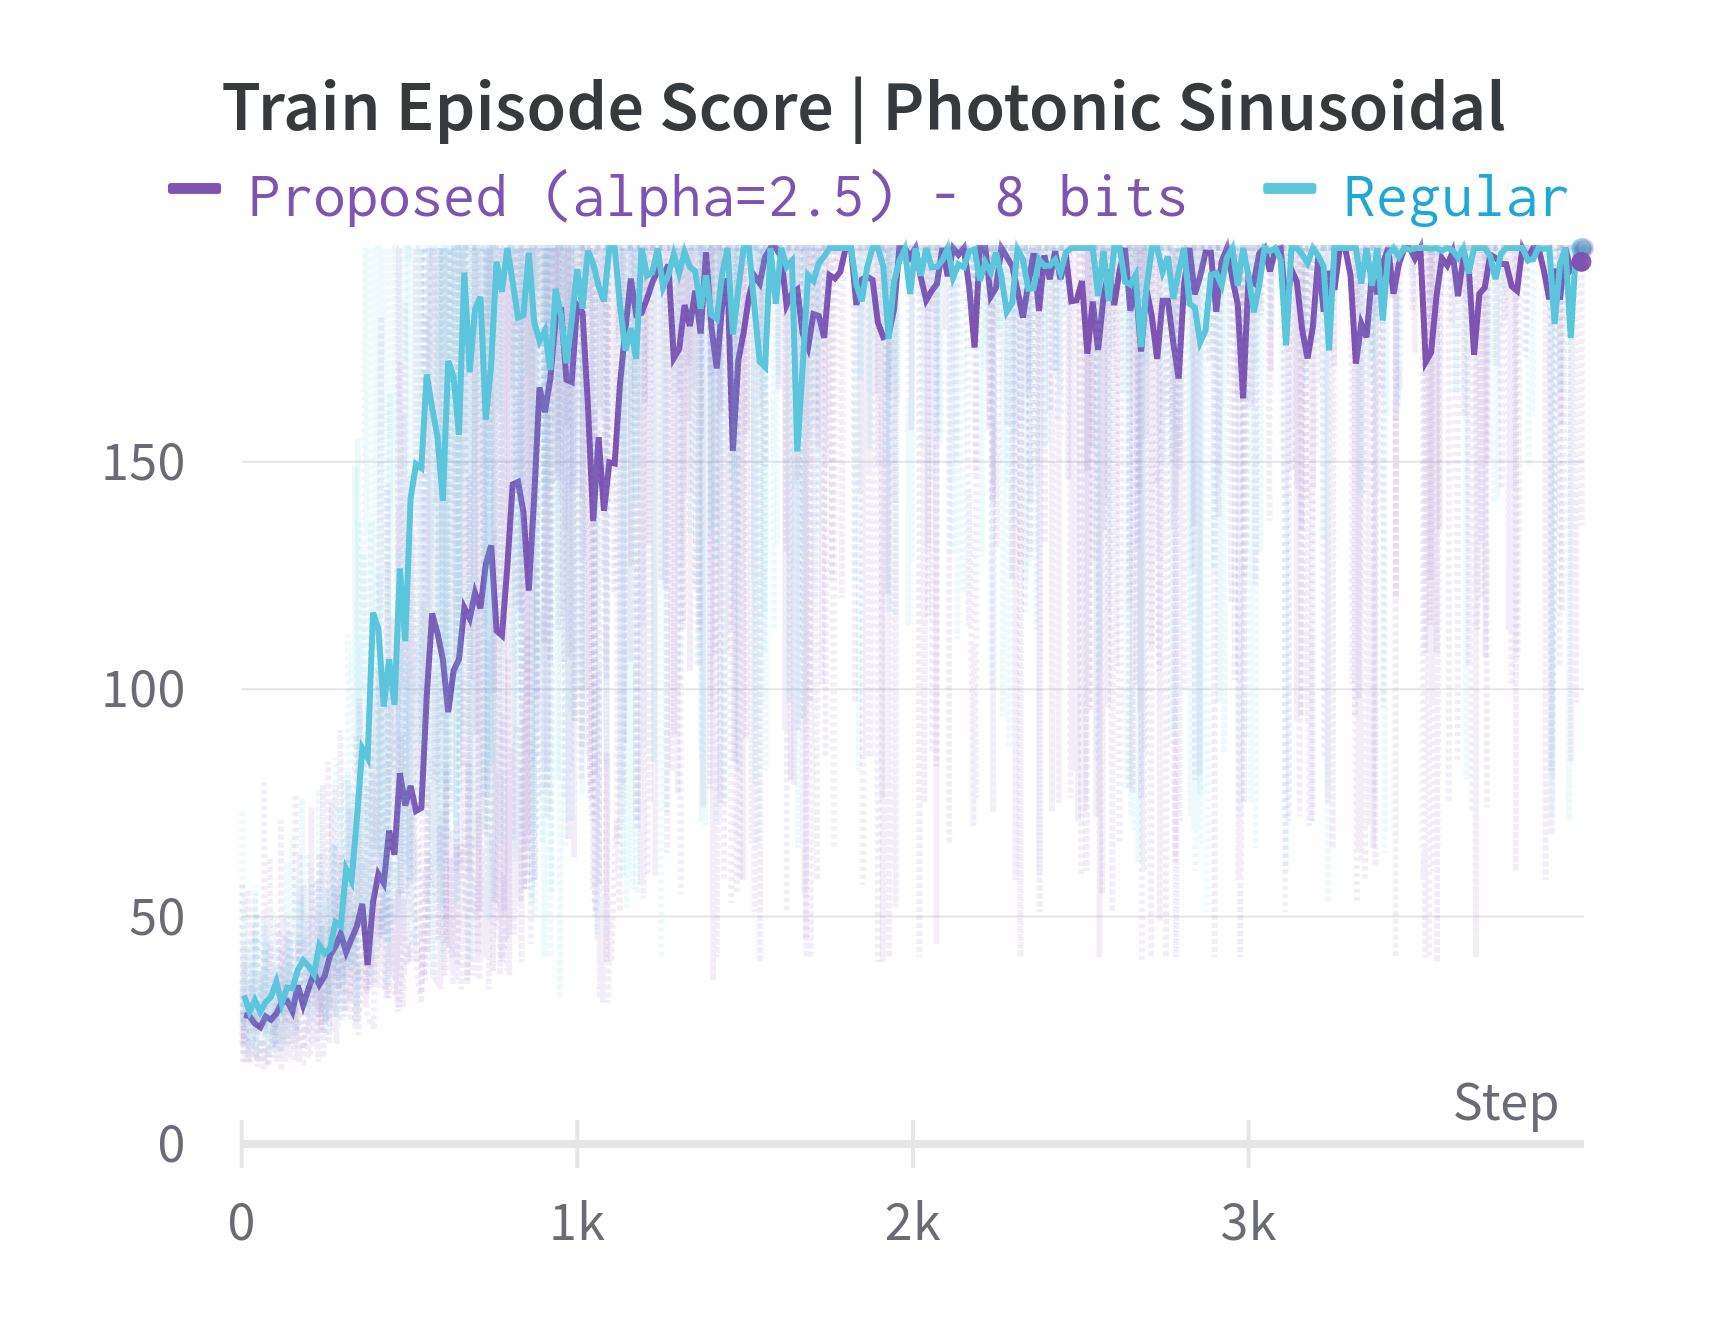
\includegraphics[width=\textwidth]{sections/2_quant/imgs/photonic_sinusoidal_8bits.png}
     \end{subfigure}
    \begin{subfigure}[b]{0.39\textwidth}
    \centering
    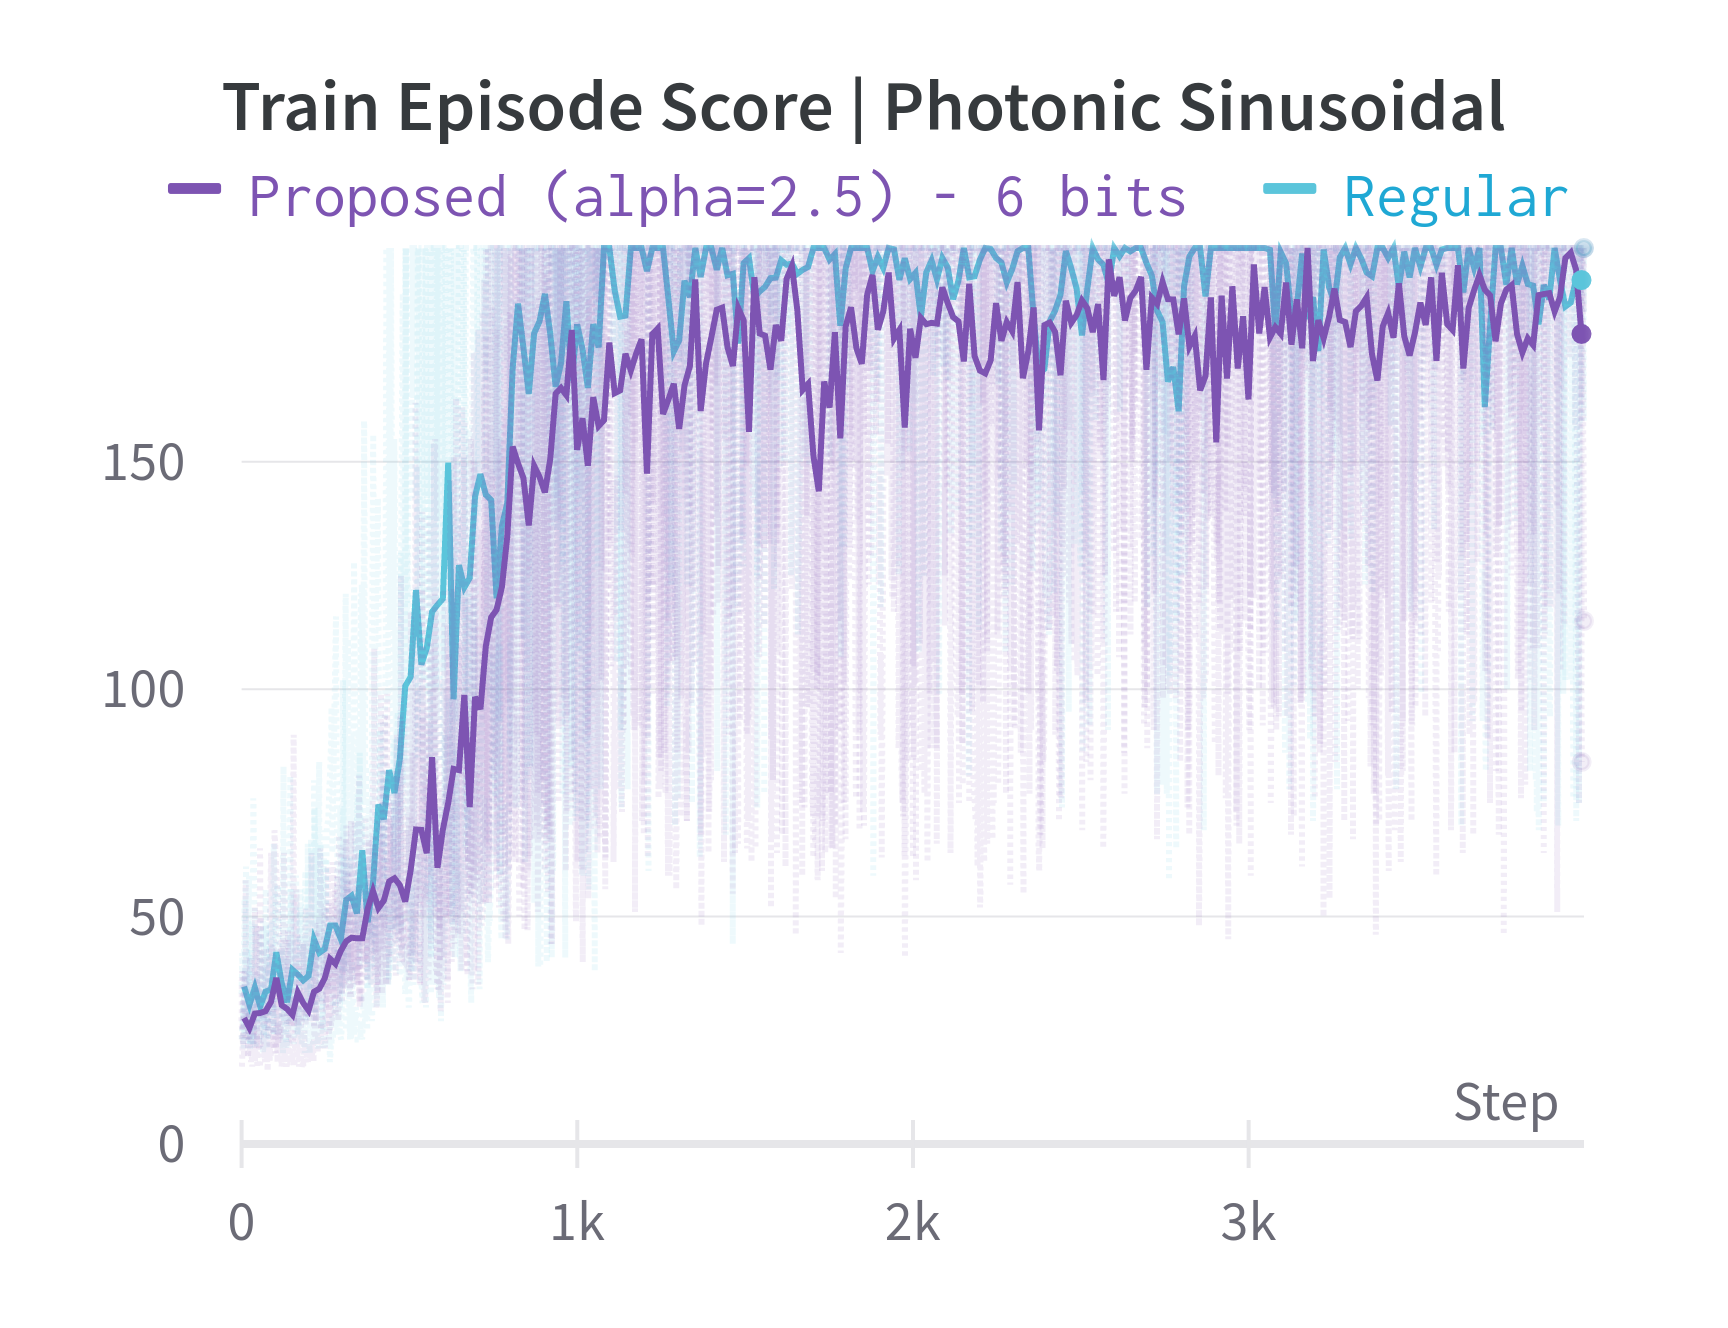
\includegraphics[width=\textwidth]{sections/2_quant/imgs/photonic_sinusoidal_6bits.png}
    \end{subfigure}\\
     \begin{subfigure}[b]{0.39\textwidth}
         \centering
         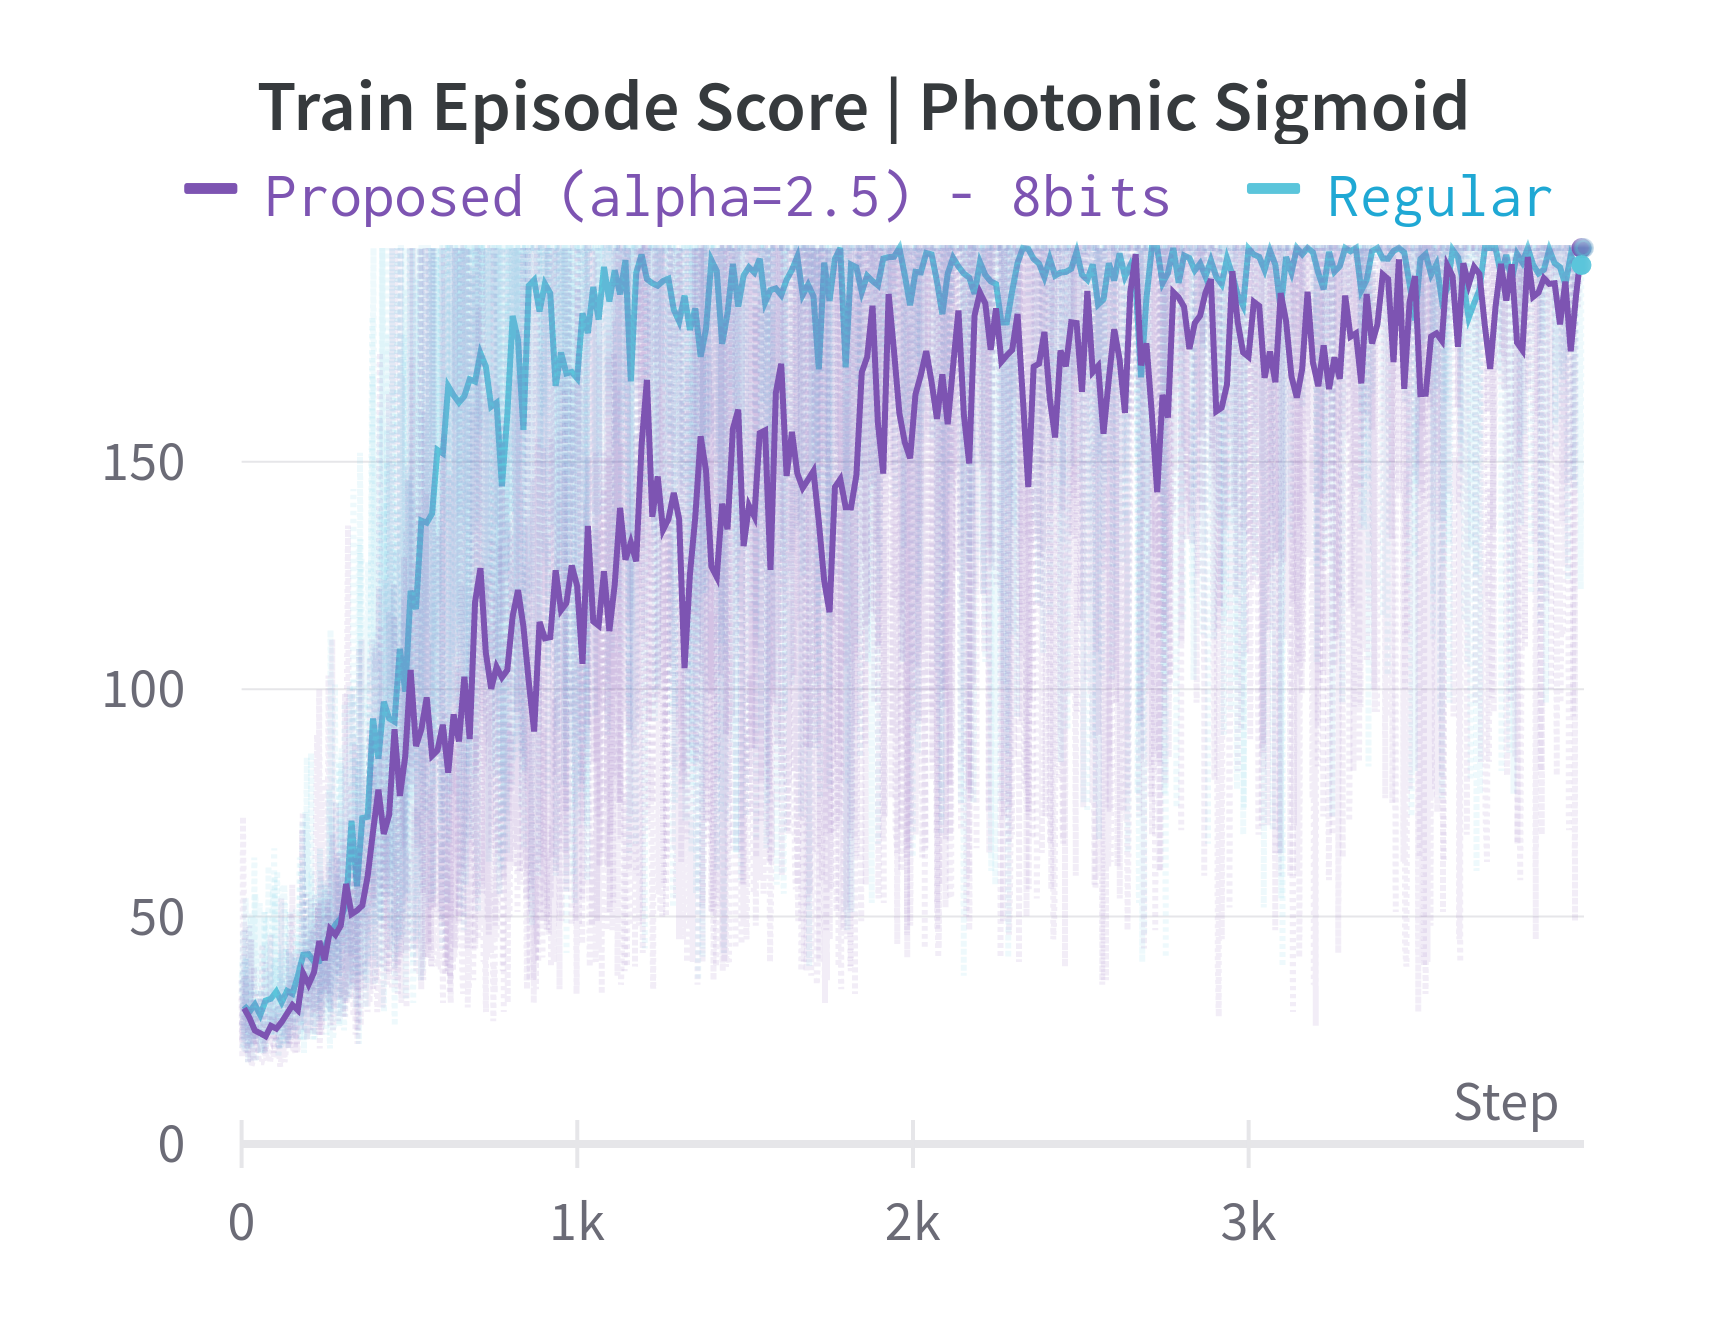
\includegraphics[width=\textwidth]{sections/2_quant/imgs/photonic_sigmoid_8bits.png}
     \end{subfigure}
     \begin{subfigure}[b]{0.39\textwidth}
         \centering
         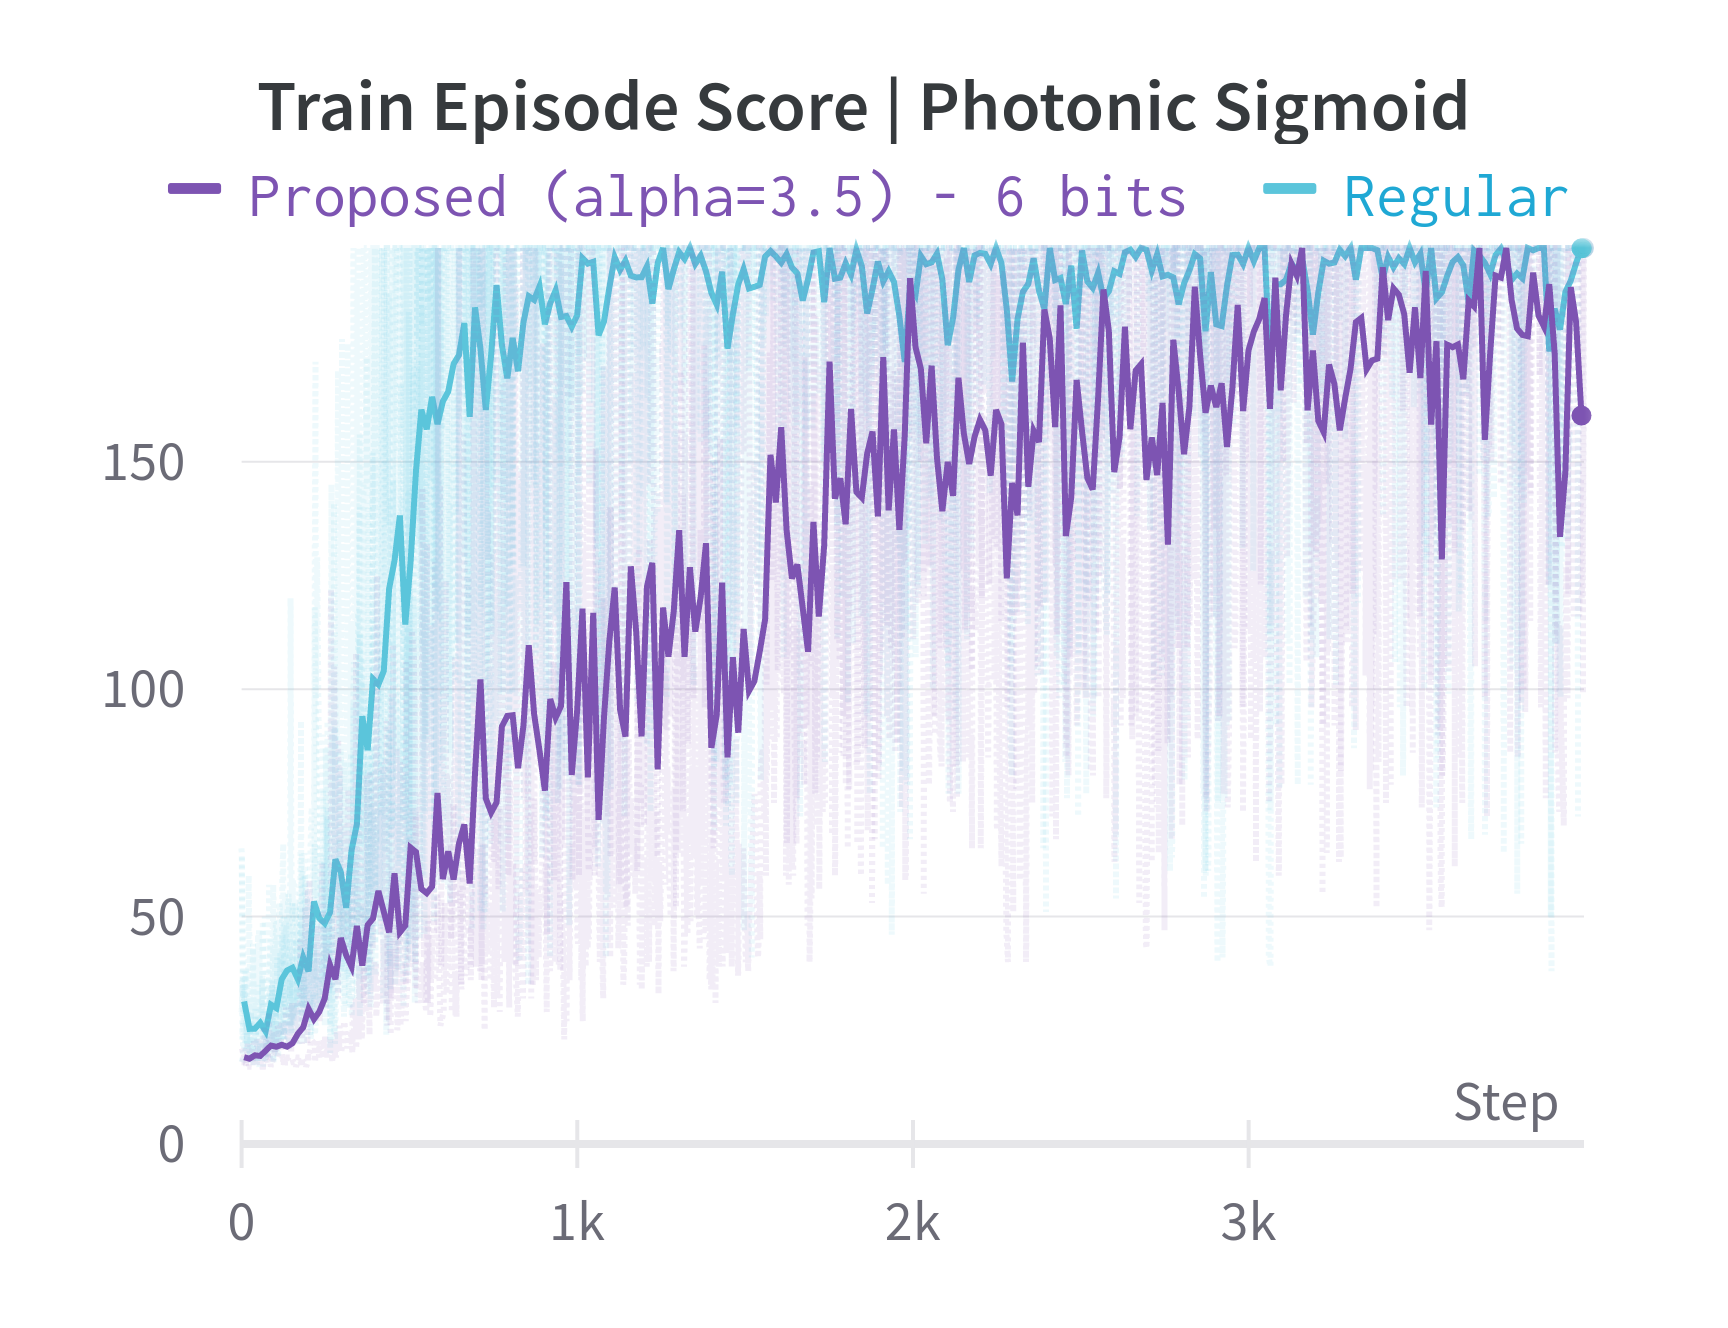
\includegraphics[width=\textwidth]{sections/2_quant/imgs/photonic_sigmoid_6bits.png}
     \end{subfigure}
    \caption{Average episode reward for each step obtained by the proposed method and regular (full resolution) training.}
    \label{fig:drl}
\end{figure}
\end{frame}

\begin{frame}{Publications}
\begin{itemize}
    \item Main Journal Publications
    \begin{itemize}
        \item {\scriptsize \textbf{Kirtas, M.}, Oikonomou, A., Passalis, N., Mourgias-Alexandris,
      G., Moralis-Pegios, M., Pleros, N. and Tefas, A., 2022. \href{https://www.sciencedirect.com/science/article/pii/S0893608022003598}{Quantization-aware training for low precision photonic neural networks.} Neural Networks, Elsevier}
    \end{itemize}
    \item Main Conference Publications 
        \begin{itemize}
        \item {\scriptsize \textbf{Kirtas, M.}, Passalis, N., Oikonomou, A., Mourgias-Alexandris, G., Moralis-Pegios, M., Pleros, N. and Tefas, A., 2022, December.\href{https://ieeexplore.ieee.org/abstract/document/10022168}{Normalized Post-training Quantization for Photonic Neural Networks.} In 2022 IEEE Symposium Series on Computational Intelligence (SSCI)} 
    \end{itemize}
\end{itemize}
\end{frame}


% \section{Mixed Precision Quantization-aware}

% \begin{frame}{Uniform Bit Resolution Limitation}
%     % Even though eliminating outlier values can lead to better performance, 

    
%     D
    
    

    
% \end{frame}

\begin{frame}{Mixed-precision Architecture}
\begin{itemize}
    \item Uniformly assigning bit resolution along layers may not be optimal %in cases where mixed precision is allowed. 
    \item Different layers varying in redundancy and contribute differently to the final performance.
    \item Identifying the bit-precision tolerance of each layer allows different computation rate~\footnote{\scriptsize Giamougiannis, G., Tsakyridis, A., Moralis-Pegios, M., Pappas, C.,
      \textbf{Kirtas, M.}, Passalis, N., Lazovsky, D., Tefas, A. and Pleros, N.,
      2023.\href{https://www.degruyter.com/document/doi/10.1515/nanoph-2022-0423/html}{ Analog
      nanophotonic computing going practical: silicon photonic deep learning
      engines for tiled optical matrix multiplication with dynamic precision.} Nanophotonics.}
\end{itemize}
    \begin{center}
        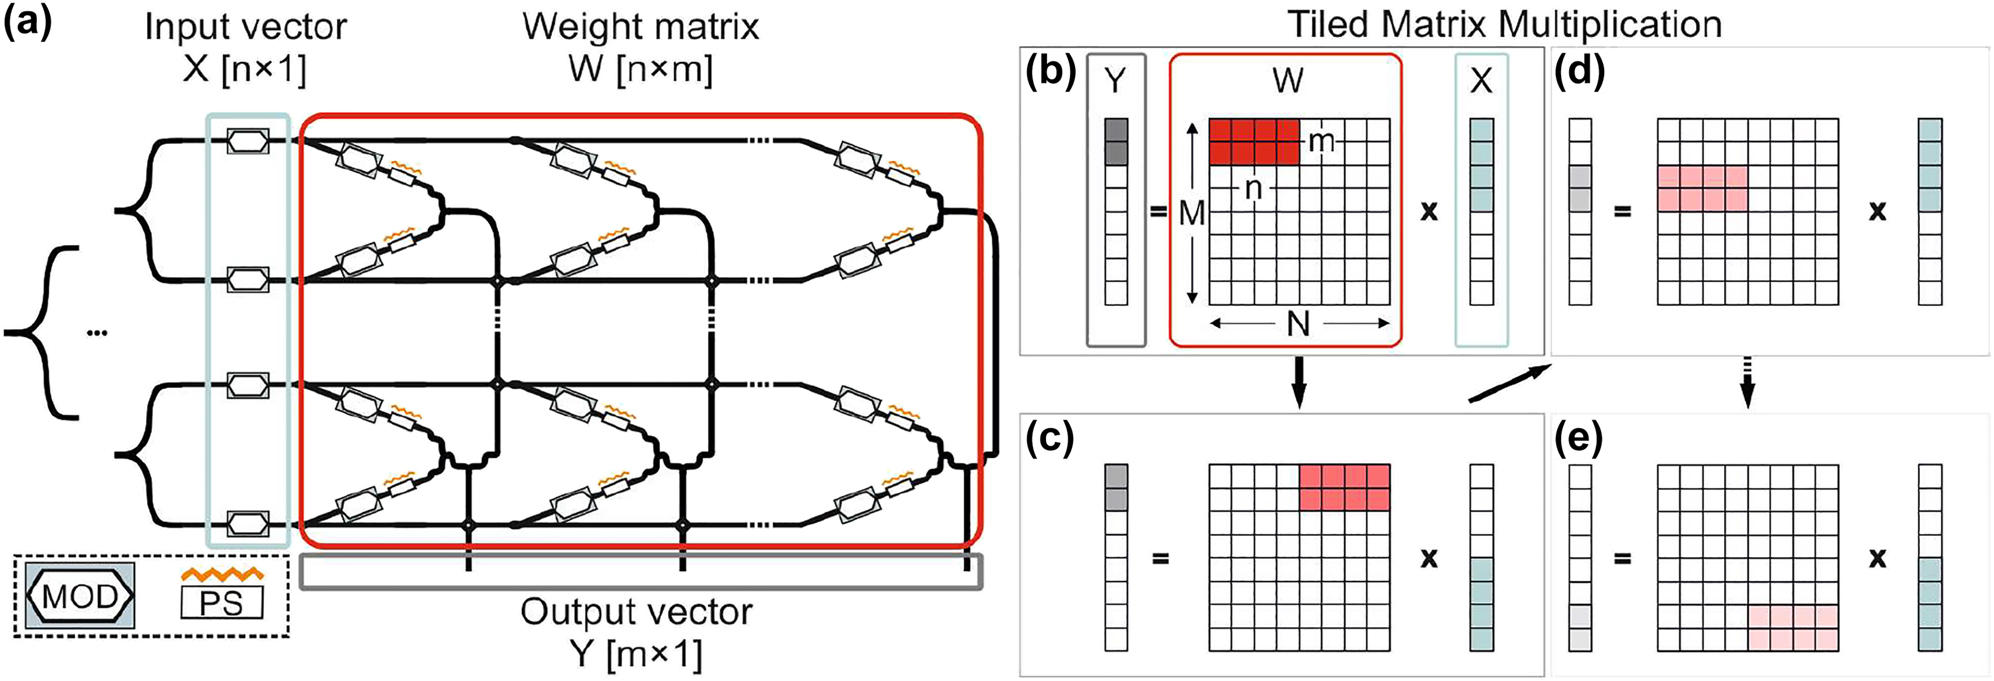
\includegraphics[width=0.8\textwidth]{sections/3_mixedquant/imgs/j_nanoph-2022-0423_fig_001.jpg}    
    \end{center}
    % of the linear operations during inference
\end{frame}

\begin{frame}{Mixed-precision Benefits}
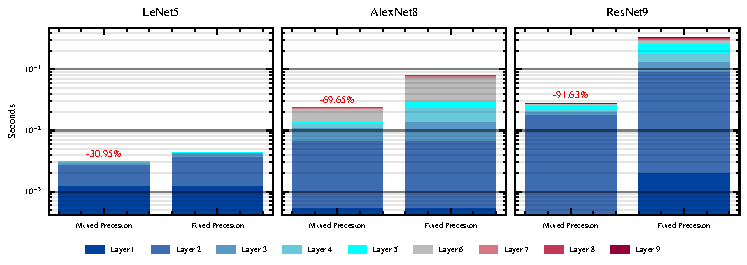
\includegraphics[width=\textwidth]{sections/3_mixedquant/imgs/exe_time.pdf}

\begin{itemize}
    \item Leads to execution time savings
    \item Lower latency
    \item Energy savings
    \item Better scalability
\end{itemize}
    
\end{frame}


\begin{frame}{Proposed Method} 
  The proposed \textbf{stochastic}, \textbf{architecture-agnostic}, \textbf{mixed-precision quantization-aware} training scheme: 
\begin{enumerate}
    \item Formalizes mixed precision quantization-aware training.
    \item \textbf{Gradually bit resolution reduction among layers.} 
    % \item Unlocks the novel mixed precision capabilities of PNNs
    \end{enumerate}
    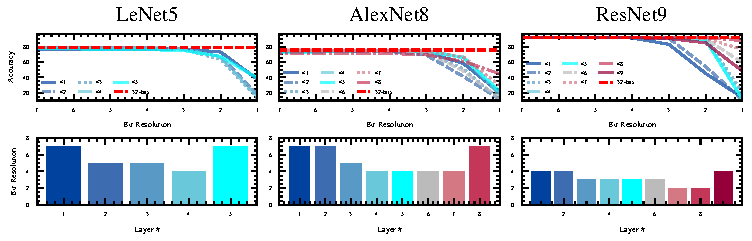
\includegraphics[width=\textwidth]{sections/3_mixedquant/imgs/dynamic_plot.pdf}
    Exploiting that the intermediate layers are more tolerant to quantization errors.
\end{frame}

\begin{frame}{Mixed Precision Quantization Formulation}
	Conceptually, the proposed method is motivated by the roulette wheel selection
  approach that is widely used in genetic algorithms.
  \begin{center}
   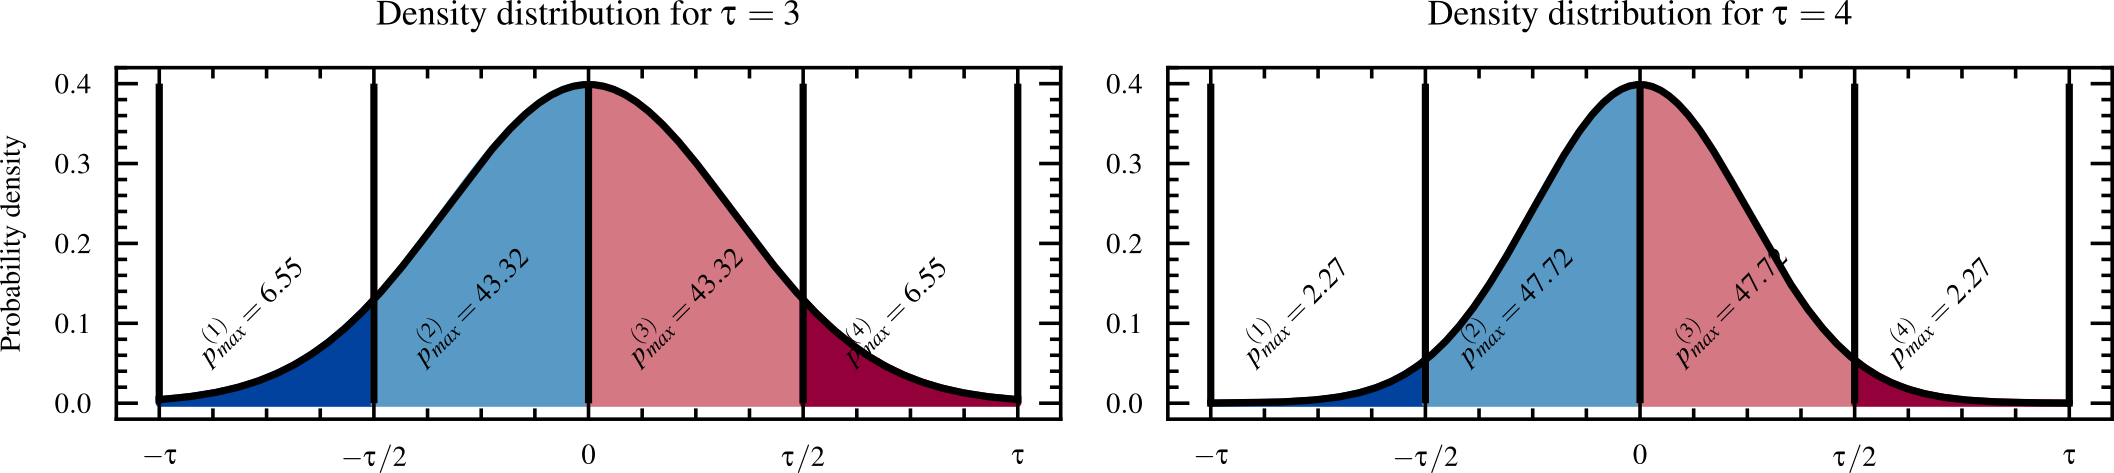
\includegraphics[width=\textwidth]{sections/3_mixedquant/imgs/gaussian_distributions.png }
  \end{center}
   \textbf{Attaches a higher probability for lower bit resolutions to intermediate layers than to outer ones following a normal distribution.}
\end{frame}



% \begin{frame}{}

% Maximum probability for a layer to reduce its bit resolution is assigned based on its position.
% \end{frame}

\begin{frame}{Maximum Probability of Each Layer}
  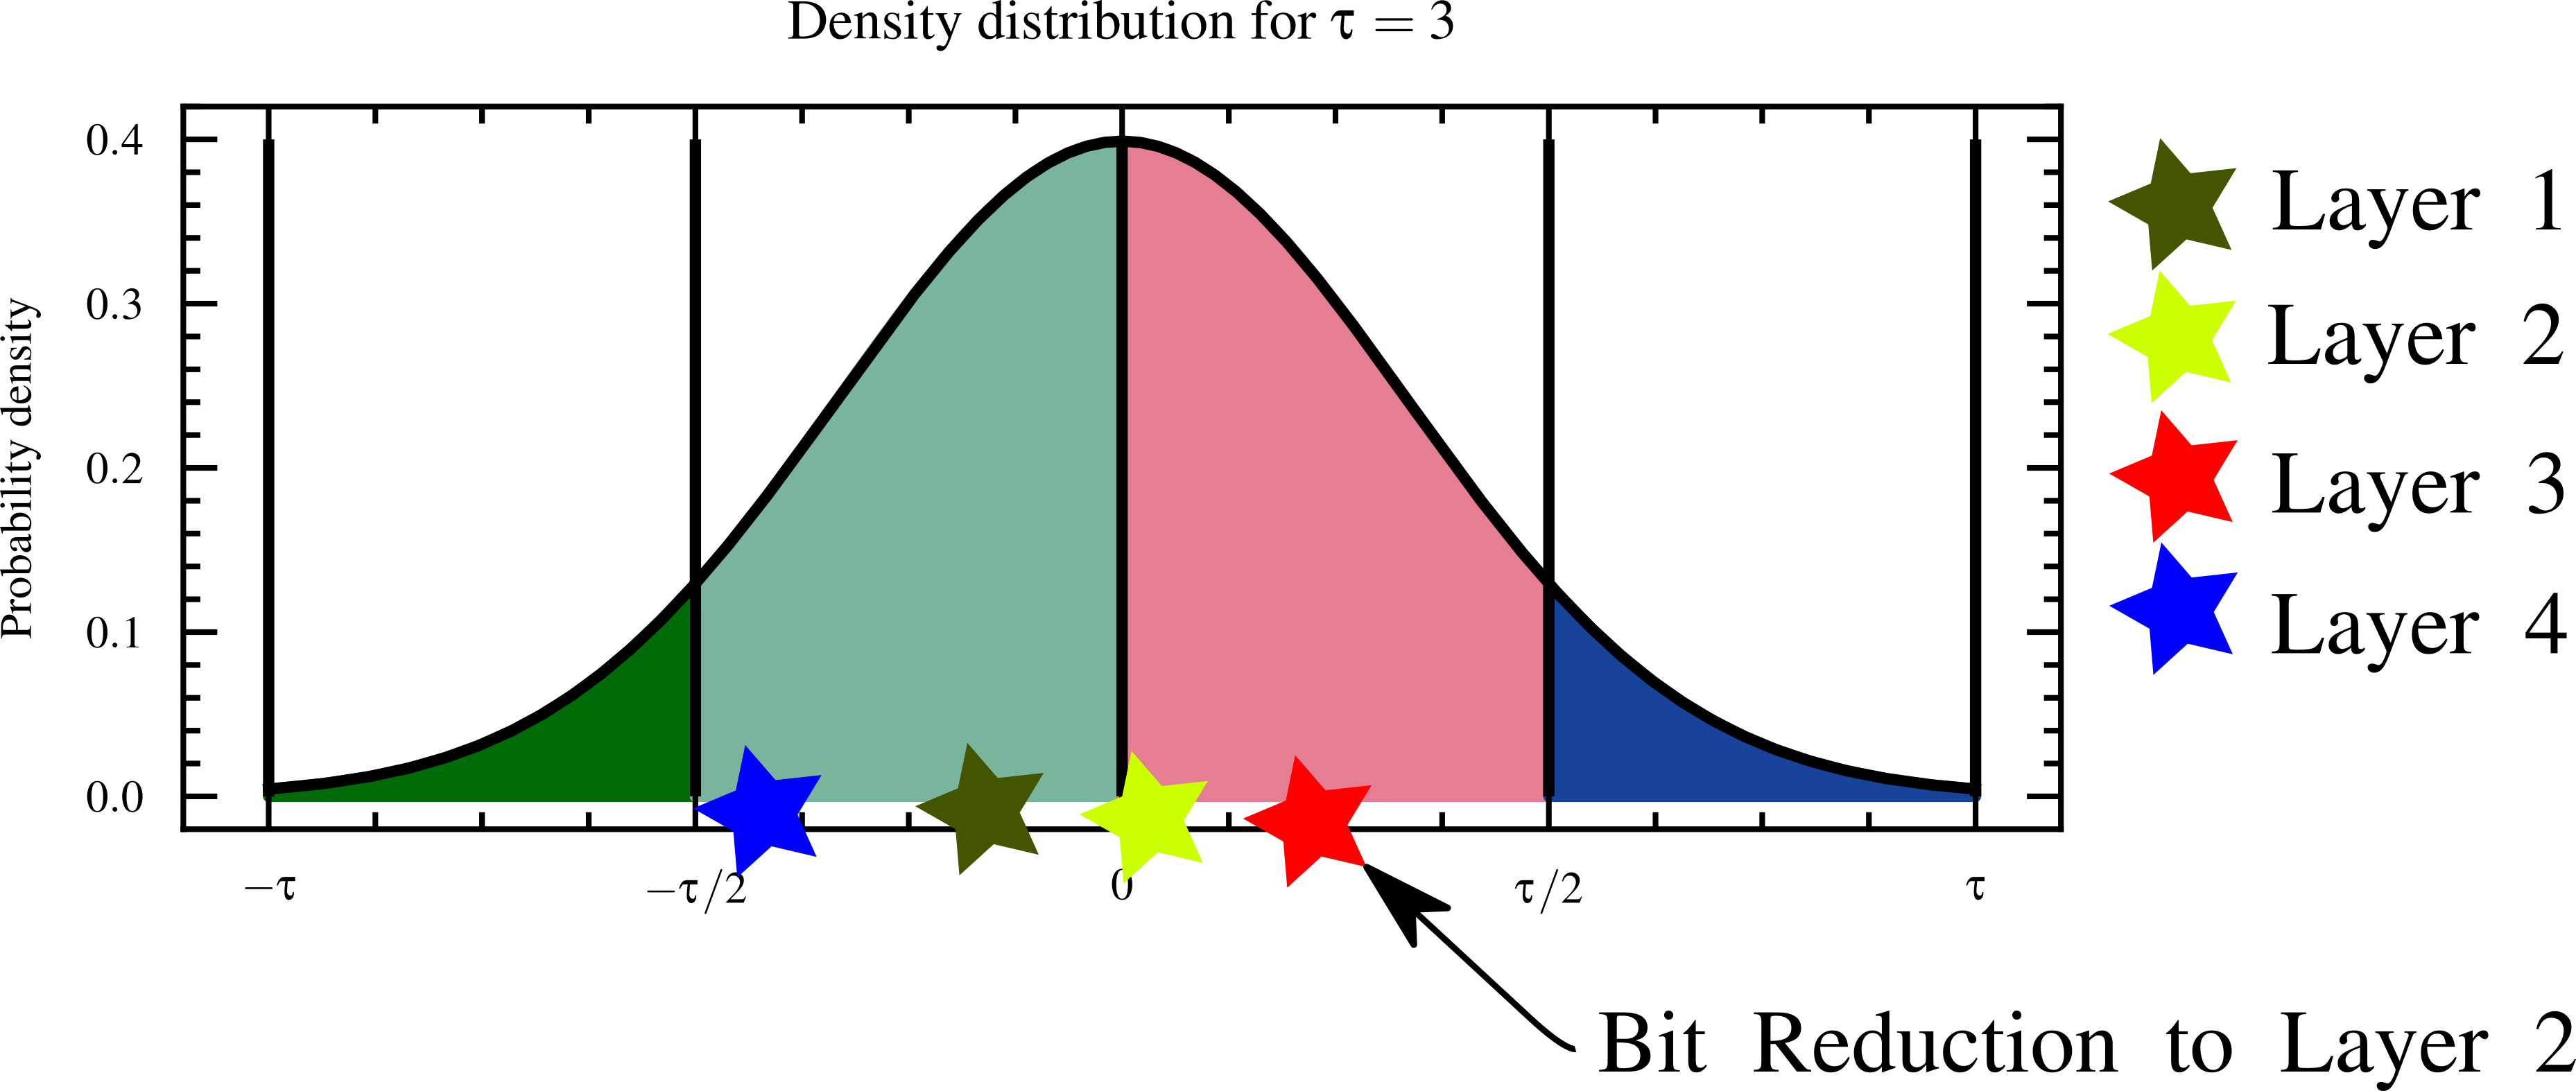
\includegraphics[width=0.8\textwidth]{sections/3_mixedquant/imgs/max_propability.png}
  
At every epoch \(t \in [0, T]\), such values as the number of layers \(\bm{u} \in
\mathbb{R}^{n}\) are drawn from the Gaussian distributions,
\begin{equation}
  \bm{u} \sim \mathcal{N}_{n}(\mu, \sigma)\in \mathbb{R}^{n},
\end{equation}
{\scriptsize  where \(n \in \mathbb{N}\) denotes the number of layers,
\(\mu \in \mathbb{R}\) and \(\sigma \in \mathbb{R}\) define the mean and
standard deviation of the Gaussian distributions, respectively.}

  
  % When the layer is at its maximum probability, a bit reduction occurs if the point \(u^{(i)}_t \sim \mathcal{N}(\mu, \sigma)\), drawn from the Gaussian distribution, is within the range
  % \(u^{(i)}_t \in [a^{(i)},a^{(i+1)})\), with \(p^{(i)}_{max, t} \in \mathbb{R}\) probability at
  % \(t\)-th timestep.
  % \begin{equation}
  %   r_{t+1}^{(i)}=\left\{
  %     \begin{array}{ll}
  %       % r_t^{(i)} & \text{if } r_t^{(i)} \leq r_{min},\\
  %   max\{r_{min}, r_t^{(i)} - r_{step}\} &  \text{if } a^{(i)} \leq u^{(i)}_t  \leq a^{(i+1)}\\
  %   r_{t}^{(i)} & \text{otherwise}.
  %     \end{array}
  %   \right .
  % \end{equation}

\end{frame}

\begin{frame}{The need for Gradual Reduction}
\begin{itemize}
    \item Providing the maximum possibility \(p^{(i)}_{max} \in \mathbb{R}\) results in low precisions in first few epochs of the training.
      \item The quantization noise will be high in the early in training where the network is unstable and not close to their convergent stage.
  \end{itemize}
  \begin{center}
  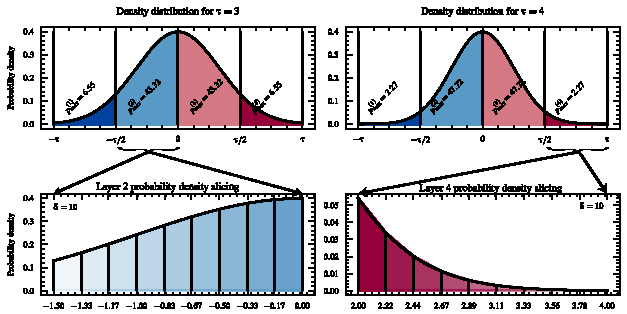
\includegraphics[width=0.8\textwidth]{sections/3_mixedquant/imgs/proposed_explained.pdf}  
  \end{center}
  A gradual bit reduction is proposed, achieved by uniformly slicing the maximum possible range of each layer.

%   \begin{itemize}
%   \item The proposed method gradually increase each layer probability until the its
%   maximum.
%   \item This is ac
%   \item  A divisor value is introduced to slice the maximum available range
%   of  \([a^{(i)},a^{(i+1)})\) in  \(\delta \in \mathbb{N}_{+}\) uniform slices
% \end{itemize}

%     \begin{enumerate}
%         \item The \textit{active} range is increased either until its maximum available range, which is equivalent to the maximum probability density
%         \item The point drawn from the Gaussian distribution \(u^{(i)}_t \sim \mathcal{N}(\mu, \sigma)\) drops within the active range \(u^{(i)}_t \in \bm{\Delta}^{(i)}_{j_t^{(i)} }\).
%     \end{enumerate}
%   \begin{equation}
% \begin{aligned}
%   \bm{\Delta}^{(i)} = [&a^{(i)}, a^{(i)} + \frac{a^{(i+1)} -
%   a^{(i)}}{\delta}, \ldots, \\
%   & a^{(i)} + \frac{(\delta-1)\left(a^{(i+1)} -
%         a^{(i+1)}\right)}{\delta}, a^{(i+1)} ] \in \mathbb{N}^{\delta}_{+},
% \end{aligned}
% \end{equation}
% {\scriptsize where the \(\bm{\Delta}^{(i)} \in \mathbb{N}^{\delta}_{+}\) is
%   called \textit{active} range of \(i\)-th 
% layer. }
\end{frame}

% \begin{frame}{Title}
%  The \(j_t^{(i)}  \in [1, \ldots, \delta]\)
% defines the epoch passed either from the start of training or from the last bit
% reduction. Therefore, at every training epoch \(t\) that the drawn value is not
% within the active range, \(u^{(i)}_{t} \notin \bm{\Delta}^{(i)}_{j_t^{(i)} }\), the
% \(j_t^{(i)} \in [1, \ldots, \delta]\) increased by a unit \(j_{t+1}^{(i)} =min\{j_{t}^{(i)} ,
% \delta\}\) if it is not equal to \(\delta \in \mathbb{N}_{+}\), increasing in this way the active
% range \(\bm{\Delta}^{(i)}_{j+1}\) by another a slice, expreseed by:   
% \begin{equation}
%     \bm{\Delta}^{(i)}_{j_{t}^{(i)}}= \left\{ \begin{array}{ll}
%          \left[a^{(i)} + \frac{(\delta-j^{(i)}_t)(a^{(i+1)} - a^{(i)})}{\delta}, a^{(i+1)}\right) & a^{(i)} \geq 0 \\[10pt]
%          \left[a^{(i)} + \frac{j^{(i)}_t(a^{(i+1)} - a^{(i)})}{\delta}, a^{(i+1)}\right) & \text{otherwise}. \\
%     \end{array}
%     \right.
%   \end{equation}
% \end{frame}

\begin{frame}{Smooth Bit Reduction}
% 	The two cases define the probability increase for both sides of the normal
% distributions, as shown in the second row of Figure~\ref{fig:proposed_exp}. If
% the range of the layer is on the negative side of the distribution, then the
% probability increases by unlocking the next slice on its right. Otherwise, if
% the layer is on the positive side of the distribution, the probability is
% increased by decreasing the lower bound to unlock another slice. In both cases,
% the probability of the \(i\)-th layer performing a bit reduction is increased,
% \(p^{(i)}_{j+1} \geq p^{(i)}_{j}\).  In the case where \(u^{(i)}_t \in
% \bm{\Delta}_{j}^{(i)}\), the active range is reset to its minimum,
% \(\bm{\Delta}^{(i)}_{j=1}\), and the method performs a bit reduction according
% to \(r^{(i)}_{t} = max\{r^{(i)}_{t-1} - r_{step}, r_{min}\}\).

The proposed method allows \textbf{smoothly increase the quantization error},
ensuring that the \textbf{noise is first introduced to more tolerant layers}. 
\begin{center}
    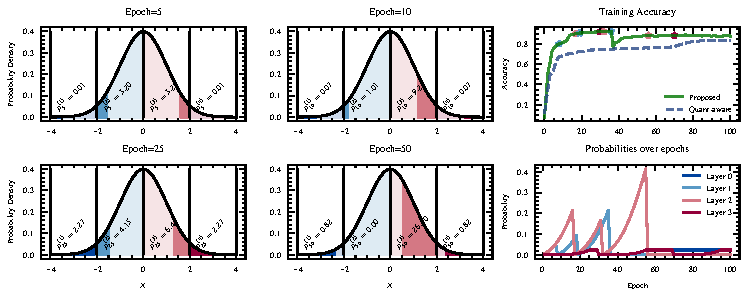
\includegraphics[width=\textwidth]{ sections/3_mixedquant/imgs/mnist_pos.pdf}
\end{center}
\end{frame}

% \begin{frame}{Probability of bit reduction}
% The probability of the \(i\)-th layer to reduce its precision by \(r_{step} \in \mathbb{N}_{+}\) bits at \(t\)-th epochs is given by:  
% \begin{equation}
%     p^{(i)}_{t} = \left\{
%     \begin{array}{ll}
%     min\left\{p^{(i)}_{max},  \frac{1}{\sqrt{2\pi}}\int_{\bm{\Delta}_{j_t^{(i)}}}e^{-z^2/2}dz\right\} & \text{if } b_{t}^{(i)} < b_{max},\\[10pt]
%     0 & \text{otherwise},
%     \end{array}
%      \right. 
% \end{equation}
% where \(j\) is calculated at every epoch \(t\) as:
% \begin{equation}
%      j_{t+1}^{(i)}=\left\{
%     \begin{array}{ll}
%     1 &  \text{if } u_{t} \in \bm{\Delta}_{j_t^{(i)}},\\
%     min\{j_t^{(i)} + 1, \delta\} & \text{otherwise},
%     \end{array}
%   \right. 
% \end{equation}
% with \(\{j_1^{(i)}=1 \mid 1 < i < n \}\). 
% \end{frame}

% \begin{frame}
% 	In this work, we used the default hyperparameter values for all experimental
% evaluation cases. More specifically, we empirically propose using a normal
% distribution with 0 mean and variance equal to 1,
% \(\mathcal{N}(\mu=0,\sigma=1)\), while setting \(\tau=3\). The gradual increment
% of probability for bit reduction of each layer depends on \(\delta\), and in
% turn, we set equal to \(\delta=M/4\), where \(M \in \mathbb{N}\) is the number of epochs.
% Finally, the bit reduction step is set to \(r_{step}=2\). It should be mentioned
% that the proposed method is presented for an even number of layers for
% simplicity, but it can be used straightforwardly for an odd number of layers
% simply by shifting the normal distribution right or left.    

% \end{frame}

% \begin{frame}{Experimental Evaluation: 4-Layer MLP in MNIST}
% 	\begin{table}[ht]
%     \resizebox{0.85\linewidth}{!}{
% \begin{tabular}{l|ccc}
%     \toprule
%          \textbf{Avg. Bits} &  \textbf{Post Quantization} & \textbf{Quant. Training} & \textbf{Proposed} \\
%      \midrule
%      \multicolumn{4}{c}{\textbf{Photonic Sinusoidal} \hspace{0.1cm} \( (\mathit{93.35\pm{0.23}}) \)}\\
%      \midrule
%      7 & $15.97\pm{2.95}$ & $92.77\pm{0.19}$ & $\bm{93.00\pm{0.09}}$\\
%      6 & $15.38\pm{2.39}$ & $92.57\pm{0.26}$ & $\bm{92.87\pm{0.20}}$\\
%      5 & $15.39\pm{2.32}$ & $92.40\pm{0.21}$ & $\bm{92.48\pm{0.20}}$\\
%      4 & $15.35\pm{5.11}$ & $91.95\pm{0.30}$ & $\bm{92.19\pm{0.22}}$\\
%      3 & $15.35\pm{2.37}$ & $85.35\pm{3.45}$ & $\bm{89.77\pm{0.66}}$\\
%      2 & $12.80\pm{1.02}$ & $64.78\pm{3.30}$ & $\bm{73.61\pm{5.85}}$\\
%      \midrule
%      \multicolumn{4}{c}{\textbf{Photonic Sigmoid} \hspace{0.1cm} \( \mathit{(92.10 \pm{0.52})} \)}\\
%      \midrule
%      7 & $86.31\pm{7.78}$ & $92.14\pm{0.18}$ & $\bm{92.44\pm{0.14}}$\\
%      6 & $82.09\pm{5.97}$ & $92.29\pm{0.37}$ & $\bm{92.37\pm{0.34}}$\\
%      5 & $82.16\pm{1.25}$ & $92.07\pm{0.32}$ & $\bm{92.12\pm{0.15}}$\\
%      4 & $70.82\pm{7.24}$ & $91.14\pm{0.22}$ & $\bm{91.68\pm{0.32}}$\\
%      3 & $54.94\pm{7.13}$ & $89.31\pm{0.44}$ & $\bm{89.35\pm{0.64}}$\\
%      2 & $28.64\pm{1.92}$ & $64.36\pm{2.95}$ & $\bm{66.10\pm{2.88}}$\\ 
%      \bottomrule
% \end{tabular}}
% \end{table}
% \end{frame}


% \begin{frame}{Experimental Evaluation: }
%   \begin{table}[ht]
% % \caption{Evaluating the proposed method on the CIFAR10 dataset using ResNet8.
% %   The table reports the average evaluation accuracy and standard deviation over
% %   5 runs. }
%     \centering
%     \resizebox{0.85\linewidth}{!}{
%       \begin{tabular}{l|ccc}
%         \toprule
%         \textbf{Bits} &  \textbf{Post Quantization} & \textbf{Quant. Training} & \textbf{Proposed} \\
%         \midrule
%         \multicolumn{4}{c}{\textbf{Photonic Sinusoidal} \hspace{0.1cm} \( (\mathit{73.14 \pm{0.60}}) \)}\\
%         \midrule
%         7 & $10.00\pm{0.00}$ & $67.56\pm{1.13}$ & $\bm{69.69\pm{0.65}}$\\
%         6 & $10.00\pm{0.00}$ & $67.07\pm{2.13}$ & $\bm{70.01\pm{0.79}}$\\
%         5 & $10.00\pm{0.00}$ & $67.87\pm{2.36}$ & $\bm{68.48\pm{0.85}}$\\
%         4 & $10.00\pm{0.00}$ & $64.20\pm{1.06}$ & $\bm{65.69\pm{2.30}}$\\
%         3 & $10.00\pm{0.00}$ & $53.71\pm{1.53}$ & $\bm{54.81\pm{5.43}}$\\
%         \midrule
%         \multicolumn{4}{c}{\textbf{Photonic Sigmoid} \hspace{0.1cm} \( \mathit{(63.31 \pm{0.63})} \)}\\
%         \midrule
%         7 & $10.00\pm{0.00}$ & $58.43\pm{2.14}$ & $\bm{62.09\pm{0.95}}$\\
%         6 & $10.00\pm{0.00}$ & $61.38\pm{2.32}$ & $\bm{62.26\pm{1.46}}$\\
%         5 & $10.00\pm{0.00}$ & $57.83\pm{1.00}$ & $\bm{61.08\pm{1.70}}$\\
%         4 & $10.00\pm{0.00}$ & $48.14\pm{2.33}$ & $\bm{52.62\pm{0.92}}$\\
%         3 & $10.00\pm{0.00}$ & $31.94\pm{3.55}$ & $\bm{39.92\pm{2.03}}$\\
%         \bottomrule
%       \end{tabular}}
%     \label{tab:2_2_cifar_exp}
%   \end{table}
% \end{frame}

\begin{frame}{ResNet8 in CIFAR10 Inference Time}
  \begin{figure}
    \centering
    \begin{subfigure}{.6\textwidth}
      \centering
      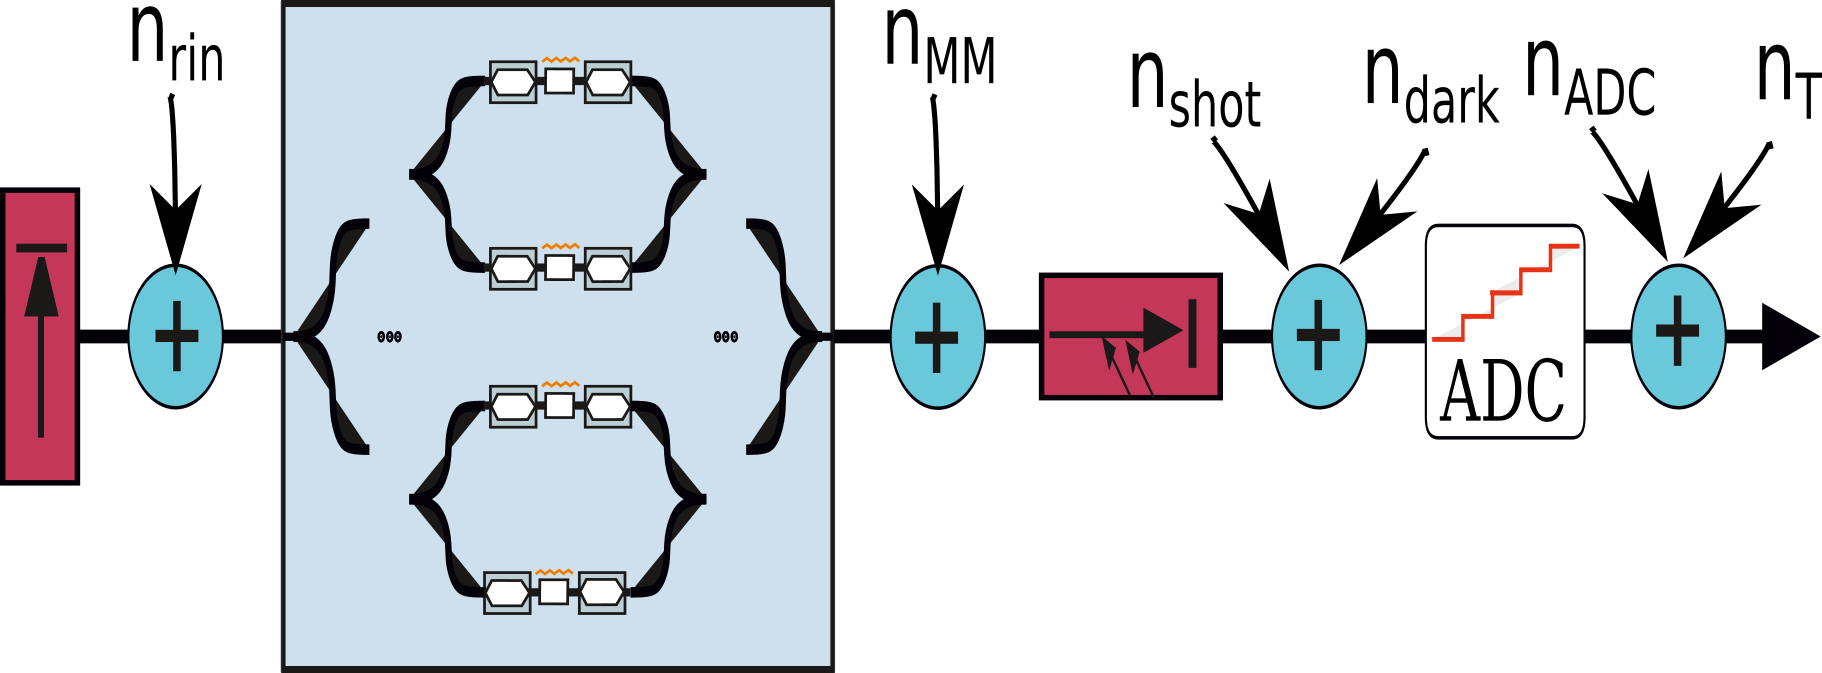
\includegraphics[width=0.9\textwidth]{sections/3_mixedquant/imgs/path1638.png}
      \caption{}
      \label{fig:noise_sources}
    \end{subfigure}\hfill
    \begin{subfigure}{.4\textwidth}
      \centering
      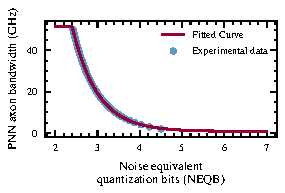
\includegraphics[width=0.8\textwidth]{sections/3_mixedquant/imgs/exe_time_fit.pdf}
      \caption{}
      \label{fig:evel_exe_time}
    \end{subfigure}
    % \caption {(a) PNN noise sources breakdown,  (b) PNN axon bandwidth versus equivalent bit resolution}
    \label{fig:background}
  \end{figure}
  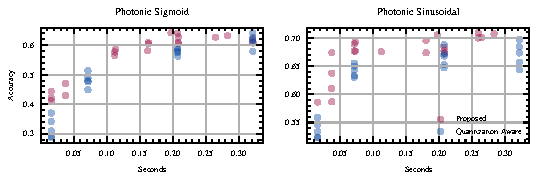
\includegraphics[width=\textwidth]{
    sections/3_mixedquant/imgs/exec_time_cifar10.pdf}      
\end{frame}


% \begin{frame}{Experimental Evaluation: RNN in FI2010}
% 	\begin{table}[ht]
% % \caption{Evaluating the proposed method on the FI2010 dataset using RNN. The
% %   table reports the average Cohen kappa metric and standard deviation on five
% %   splits in 3 evaluation runs.}
%     \centering
%     \resizebox{0.9\linewidth}{!}{
% \begin{tabular}{l|ccc}
%     \toprule
%          \textbf{Bits} &  \textbf{Post Quantization} & \textbf{Quant. Training} & \textbf{Proposed} \\
%      \midrule
%      \multicolumn{4}{c}{\textbf{Photonic Sinusoidal} \hspace{0.1cm} \( (\mathit{0.1637\pm{0.0061}}) \)}\\
%      \midrule
%      7 & $0.1469\pm{0.0032}$ & $0.1694\pm{0.0019}$ & $\bm{0.1730\pm{0.0006}}$\\
%      6 & $0.1433\pm{0.0056}$ & $0.1682\pm{0.0072}$ & $\bm{0.1724\pm{0.0003}}$\\
%      5 & $0.1400\pm{0.0057}$ & $0.1659\pm{0.0080}$ & $\bm{0.1703\pm{0.0009}}$\\
%      4 & $0.1391\pm{0.0159}$ & $0.1602\pm{0.0033}$ & $\bm{0.1656\pm{0.0032}}$\\
%      3 & $0.0388\pm{0.0058}$ & $0.1411\pm{0.0075}$ & $\bm{0.1427\pm{0.0067}}$\\
%      \midrule
%      \multicolumn{4}{c}{\textbf{Photonic Sigmoid} \hspace{0.1cm} \( \mathit{(0.1395\pm{0.0047})} \)}\\
%      \midrule
%      7 & $0.1355\pm{0.0036}$ & $0.1375\pm{0.0016}$ & $\bm{0.1392\pm{0.0044}}$\\
%      6 & $0.1355\pm{0.0009}$ & $0.1370\pm{0.0050}$ & $\bm{0.1398\pm{0.0010}}$\\
%      5 & $0.1391\pm{0.0026}$ & $0.1364\pm{0.0030}$ & $\bm{0.1404\pm{0.0005}}$\\
%      4 & $0.1124\pm{0.0035}$ & $0.1372\pm{0.0046}$ & $\bm{0.1388\pm{0.0013}}$\\
%      3 & $0.0871\pm{0.0017}$ & $0.1223\pm{0.0004}$ & $\bm{0.1226\pm{0.0007}}$\\
%      \bottomrule
% \end{tabular}}
% \end{table}
% \end{frame}

\begin{frame}{Publications}
\begin{itemize}
    \item Main Journal Publications
    \begin{itemize}
        \item {\scriptsize\textbf{Kirtas, M.}, Passalis, N., Oikonomou, A., Moralis-Pegios, M.,
      Giamougiannis, G., Tsakyridis, A., Mourgias-Alexandris, G., Pleros, N. and Tefas, A., 2023. \href{https://link.springer.com/article/10.1007/s00521-023-08848-8}{Mixed-precision quantization-aware training for photonic neural networks}. Neural Computing and Applications, Springer}
    \end{itemize}
    \item Main Conference Publications 
        \begin{itemize}
        \item {\scriptsize \textbf{Kirtas, M.}, Passalis, N., Oikonomou, A., Moralis-Pegios, M.,
      Giamourgiannis, G., Tsakyridis, A., Mourgias-Alexandris, G., Pleros, N. and Tefas, A., 2023, September.
      \href{https://ieeexplore.ieee.org/document/10285966}{Quantization-Aware Training for Mixed Precision Photonic Neural Networks.} In 2023 IEEE 33rd International Workshop on Machine Learning for Signal Processing (MLSP)} 
    \end{itemize}
\end{itemize}
\end{frame}

\section{Non-negative post-initialization}

%%%%%%%%%%%%%%%%%%%%%%%%%%%%%%%%%%%%%%%%%%%%%%%%%%%%%%%%%%%%%%%%%%%%%%%%%%%%%%%%%%%%%%%%%%%%%%%%%%%% 
\begin{frame}{Proposed Method}

  
  The proposed method can be applied on top of any existing initialization
  scheme.

  \begin{itemize}
  \item Unlocks the potential of non-negative neural networks
  \item Ensures high variance in the activation distribution
  \item Gradient propagation during the initial stage of training
  \item Increase the expressivity of the non-negative constrained models
  \end{itemize}
\end{frame}

% \begin{frame}{Novelties}
%     \begin{itemize}
%         \item The proposed framework allows one to apply it in traditionally used large architectures without any major change and performance degradation
%         \begin{itemize}
%             \item based on the non-negative isomorphic representation
%     of traditional models.
%         \end{itemize}
%         \item Investigates multiplicative updates in the context of non-negative training
%         \item Studying the isomorphism of the networks and proposing a structured methodology to acquire their nonnegative equivalent
%     \end{itemize}
% \end{frame}

\begin{frame}{On the Difficulty of Training Non-negative Neural Networks}
  % Conceptually, ANNs project the input features to a latent dimensional space,
  % aiming to represent them in a more separable way, seeking a hyperplane
  % decision boundary that can classify them in an optimal way. However,
  
\textbf{Classifying non-negative features}, even when they are linearly separable, is
  often \textbf{impossible when using non-negative parameters} for a linear classifier.

  \begin{equation}
    x_1 = - \frac{w_0}{w_1}x_0 - \frac{b}{w_1} \in \mathbb{R},
    \label{eq:reg_db}
  \end{equation}
  {\scriptsize where \(x_i \in [0, 1]\) is the input, \(w_i \in \mathbb{R}\)  and \(b\in
  \mathbb{R}\) are the weights and biases of the classifier, respectively, and
  \(i\in \{0, 1\}\). }

\begin{center}
	  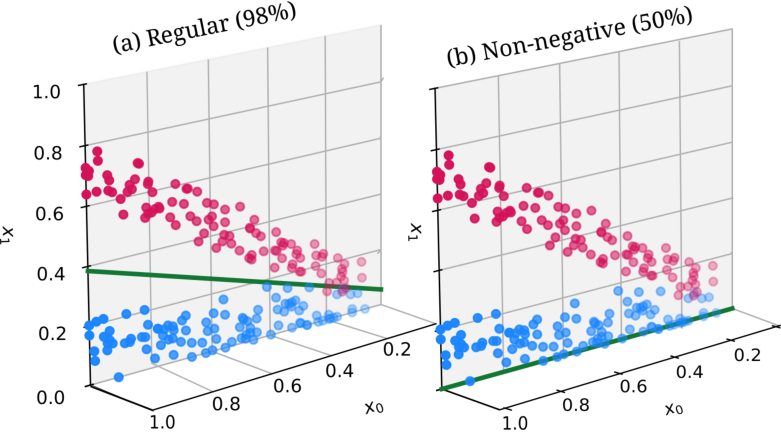
\includegraphics[width=0.6\textwidth]{sections/4_nn/imgs/training_issue.pdf}
\end{center}


  %  We can easily conclude that there is a positive slope decision, with the slope
  %  given by \(m=-w_{0}/w_{1}\), which requires a negative weight.

  %  \begin{itemize}
  % \item   In fact, training the linear classifier, using SGD, a positive slope decision
  % boundary is obtained achieving optimal performance with \(w_0<0\).
  % \item  On the other hand, constraining the classifier to
  % non-negative parameters results in a negative slope decision boundary that
  % cannot discriminate between the two classes
% \end{itemize}
\end{frame}

% \begin{frame}
  

% \end{frame}

% \begin{frame}{Isomorphism in Neural Networks}
% \textbf{Challenging computational tasks} can be easily solved by \textbf{changing the coordinate system}
% \begin{center}
%     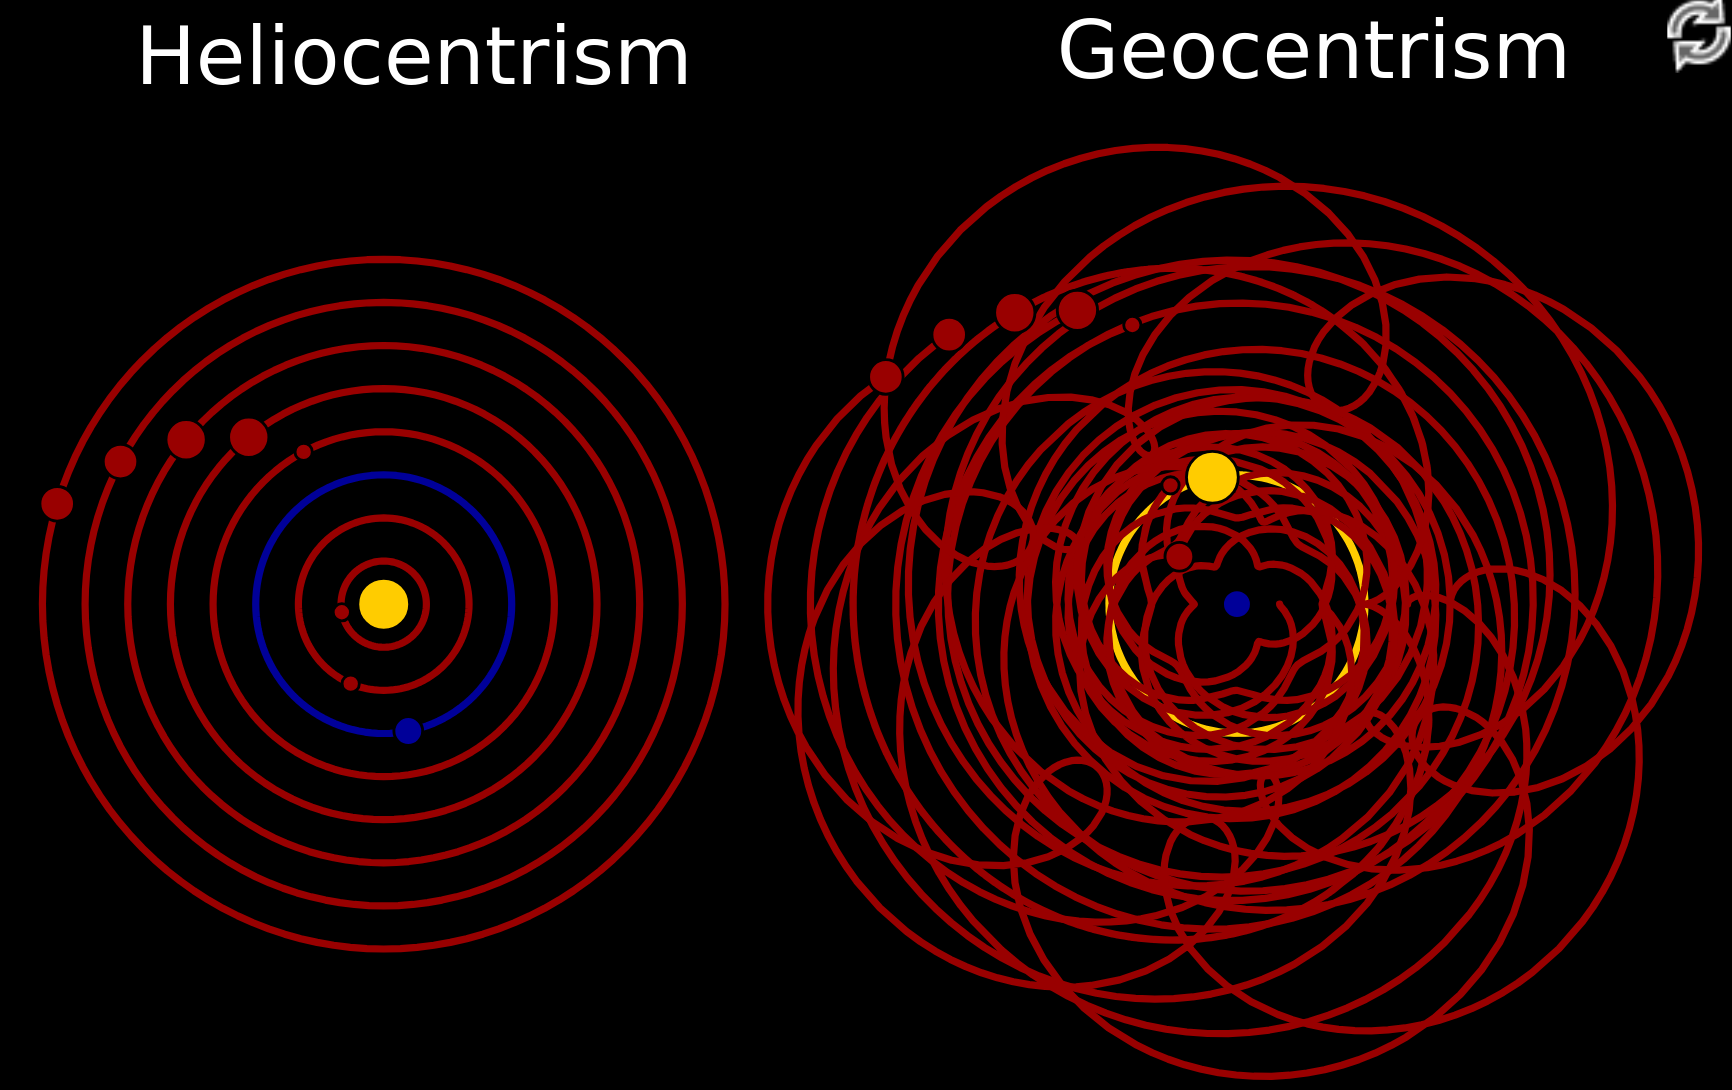
\includegraphics[width=0.45\textwidth]{sections/4_nn/imgs/Selection_548.png}
% \end{center}
% \textbf{Considering isomorphism}, it is claimed that \textbf{ an equivalent classifier with non-negative parameters exists}, producing the \textbf{same classification outcome as the original one.}
% \end{frame}

\begin{frame}{Transformation}

  \begin{columns}[T]
    \begin{column}{0.46\textwidth}
      The original task and classifier can be transformed, by \textbf{shifting
        and rotating the points and the decision boundary}, getting an
      equivalent non-negative classifier\textbf{, using only non-negative
        parameters.} The acquired non-negative classifier results in the decision boundary given by
      \begin{equation}
        x_1 =-\frac{\left|w_{0}\right|}{w_{1}} x_0' -\frac{b-a\left|w_{0}\right|}{w_{1}} \in \mathbb{R}
      \end{equation}
      {\scriptsize where \(w_0 < 0\), \(w_1 > 0\), \(a=1\) and
        \(x_0'=\left(a-x_0\right)\).}
      % The non-negative classifier leads to a rotated decision boundary and is equal to
      % the original classifier performance.
    \end{column}
    \begin{column}{0.46\textwidth}
      \begin{center}
        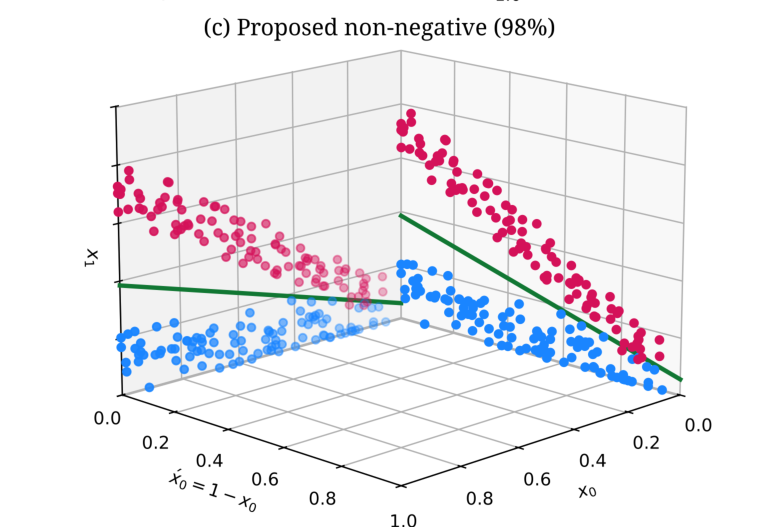
\includegraphics[width=\linewidth]{sections/4_nn/imgs/proposed_transformation.pdf}
      \end{center}

    \end{column}
  \end{columns}

  




\end{frame}

\begin{frame}{Definition of Fully-connected Layer}
  Let \(\bm{z}^{(j)} \in \mathbb{R}^{N_{j}}\) be the output of the linear part
  of the \(j\)-th layer of a neural network architecture, where the linear
  function is denoted as
  \(f^{(j)}(\cdot):\mathbb{R}^{N_{j-1}}\rightarrow\mathbb{R}^{N_{j}}\), given by 
  \begin{equation}
    \label{eq:linear}
    \bm{z}^{(j)} = f^{(j)}(\bm{x}^{(j)}) = \bm{W}^{(j)}\bm{x}^{(j)} + \bm{b}^{{(j)}} \in \mathbb{R}^{N_{j}},
  \end{equation}
  {\scriptsize where \(\bm{W}^{(j)} \in \mathbb{R}^{N_{j} \times  N_{j-1}}\),
    \(\bm{b}^{(j)} \in \mathbb{R}^{N_j}\), and \(\bm{x}^{(j)} \in
    \mathbb{R}^{N_{j-1}}\).}

  Assuming that an activation function \(\phi(\cdot): \mathbb{R}^{N_j} \rightarrow \mathbb{R}^{N_j}_{+}\), where \(\mathbb{R}_{+}\) denotes the set of positive real values, the output of the \(j\)-th layer is given by:
  \begin{equation}
    \label{eq:activation}
    \bm{y}^{(j)} = \phi^{(j)}(\bm{z}^{(j)}) \in \mathbb{R}^{N_j}_{+}.
\end{equation}
\end{frame}

% \begin{frame}{Definition Linear Neuron}
% Let \(z_i \in \mathbb{R}\) the \textbf{response of the linear part }of the \(i\)-th \textbf{neuron} of a fully connected
%   layer, where the linear function is denoted by \(u_{i}(\cdot): \mathbb{R}^{M}
%   \rightarrow \mathbb{R}\) and \(i = 1 \ldots N\), given by:  

%   \begin{equation}
%     \label{eq:linear_pass}
%     z_i = u_i(\bm{x}) = \sum_{j=1}^{M}{w_{ij}} x_j + b_i  \in \mathbb{R}, 
%   \end{equation}
%   {\scriptsize where \(\bm{w}_i \in \mathbb{R}^{M}\), \(b_i \in \mathbb{R}\) and \(\bm{x} \in
%   \mathbb{R}^{M}\) are the weight, bias, and input vectors of the \(i\)-th
%   neuron, respectively.}

%     Assuming an\textbf{ activation function }\(g(\cdot): \mathbb{R}
%   \rightarrow \mathbb{R}_{+} \), where \(\mathbb{R}_{+}\) denotes the set of
%   non-negative real values, the output of the \(i\)-th neuron is: 
%   \begin{equation}
%     y_i = g(z_i) \in \mathbb{R}_{+}.
%   \end{equation}

% \end{frame}

\begin{frame}{Transformation: Input Rotation}

\noindent
\begin{minipage}{.7\textwidth}
  Rotate the input multidimensional-space to a non-negative axis,
  projecting the weights that were originally initialized as negative onto the
  \begin{equation}
     \mathbbm{1}_{N_{j-1}}\alpha^{(j)} - \bm{x}^{(j)} \in [0,
  \alpha]^{{N_{j-1}}}-\text{axis}
  \end{equation}

  {\scriptsize with \(\mathbbm{1}_{N_{j-1}} \in [1, \ldots, 1]^{N_{j-1}}\) and \(\alpha^{(j)}
  \geq max(\mathcal{X}^{(j)})\) denotes the rotation constant of the layer  and
  \textit{max} denotes the maximum element in the feasible set \(\{x^{(j)}_{i} :
  \bm{x}^{(j)} \in [x_{min}, x_{max}]^{N_{j-1}} \subset
  \mathbb{R}_{+}^{N_{j-1}} \} \).}


  % . The , defined as \(\mathcal{X}^{(j)}\). The existence of the rotation constant \(\alpha^{(j)}\) requires a closed interval of \(\mathcal{X}^{(j)}\) that can be easily achieved in input through normalization or by considering a bounded activation function in the intermediate layers.
%       This allows us to \textbf{rotate} the \textbf{input feature space}, as
% \begin{equation*}
% \label{eq:rotated_input}
%     x_j' = f(x_j) = 
%     \begin{cases}
%         \alpha - x_j & \text{if } w_{ij} <  0\\
%         x_j     & \text{otherwise},
%     \end{cases}
% \end{equation*}
% {\scriptsize where \(x_j' \in \mathbb{R}_{+}\).} 
\end{minipage}% This must go next to `\end{minipage}`
\begin{minipage}{.3\textwidth}
    \begin{flushright}
    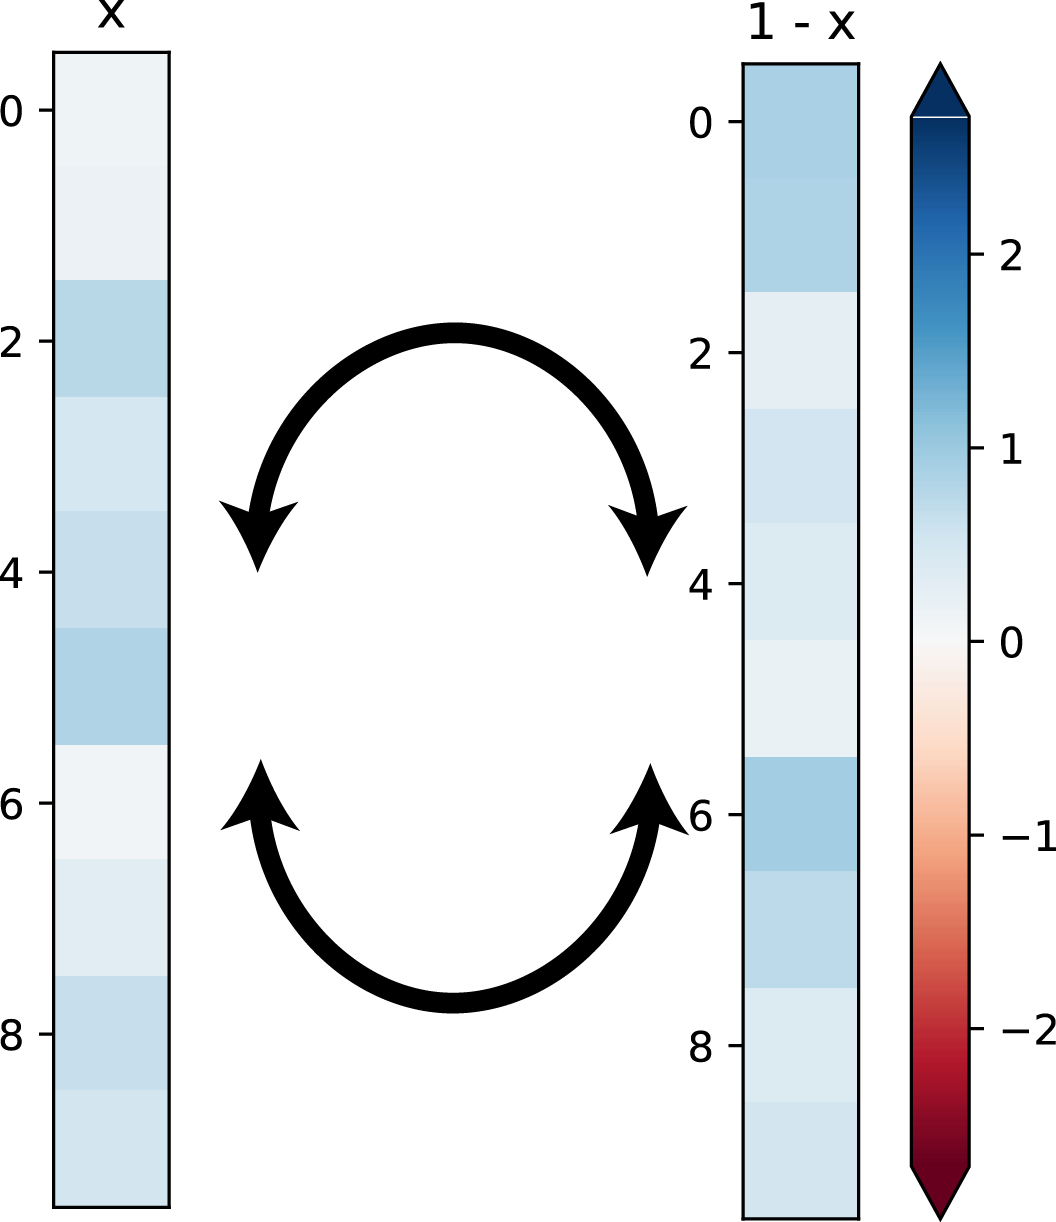
\includegraphics[width=0.8\linewidth]{sections/4_nn/imgs/x_1.png}
    \end{flushright}
\end{minipage}

\end{frame}


\begin{frame}{Transformation: Weight shifting}

  The initialized non-negative weights will retain their initial variance in those two axes as a projection
\begin{equation}
    \label{eq:trans_1}
    \bm{z}^{(j)} = \bm{W}_{-}^{(j)}(\mathbbm{1}_{N_{j-1}}\alpha^{(j)} - \bm{x}^{(j)}) + \bm{W}^{(j)}_{+}\bm{x}^{(j)} + \bm{b}^{'}{}^{(j)} \in \mathbb{R}_{+}^{N_j} 
\end{equation}
{\scriptsize where \(\bm{W}_{+}^{(j)} + \bm{W}_{-}^{(j)} = |\bm{W}^{(j)}|\) with
\(|\bm{W}^{(j)}| \in \mathbb{R_{+}}^{N_{j} \times N_{j-1}}\) denotes the
absolute value of the original weight matrix and \(\bm{b}^{'}{}^{(j)}\in
\mathbb{R}^{N_{j}}_{+}\) the bias vector. }

% \vspace{10pt}
% 	Linear neuron can be expressed as:
%   \begin{equation}
%     \label{eq:transformation_3}
%     z'_i = \sum_{\{j |w_{ij} < 0\}}|w_{ij}|(\alpha - x_{j}) + \sum_{\{j |w_{ij} > 0\}}w_{ij}x_j + \tilde{b}_i \in \mathbb{R}.
%   \end{equation} 

   \begin{center}
       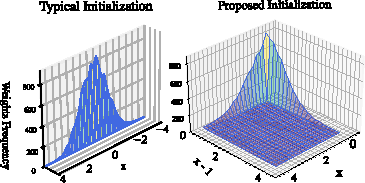
\includegraphics[width=0.6\linewidth]{sections/4_nn/imgs/wcci_proposal_v3.pdf}
   \end{center}

%  Both \(\bm{W}^{(j)}_{-} = \max(0,
% -\bm{W}^{(j)})\in \mathbb{R}_{+}^{N_{j} \times N_{j-1}}\) and \(\bm{W}_{+}=
% \max(0, \bm{W}^{(j)}) \in \mathbb{R}_{+}^{N_{j} \times N_{j-1}}\) are sparse
% matrices, each containing \(\approx 50 \%\) zero values.

 \end{frame}

 \begin{frame}{Transformation: Bias Integration}
   % The bias term can be initialized to any non-negative vector
   % \(\bm{b}^{'}{}^{(j)}\in \mathbb{R}^{N_j}_{+}\), however, this will lead to a
   % different variance in the output of the activation function, undermining the
   % applied initialization scheme.


   % To overcome this and ensure that the variance
   % of the activation values is preserved during training, we propose
   % initializing the biases based on the initialized weights and acquiring the
   % same variance in the activation distribution. More specifically, we propose
   % to accumulate

   The applied positive rotation of the weights in the
   \((\mathbbm{1}_{N_{j-1}}\alpha^{(j)} - \bm{x}^{(j)})\) axis is accumulated in the bias term
   and integrate it into a shifted activation function. Thus, the bias vector is
   initialized as  
   \begin{equation}
     \label{eq:new_bias}
     \bm{b}^{'}{}^{(j)} = \tilde{\bm{b}}^{(j)} + \mathbbm{1}_{N_{j}} c^{(j)} \in \mathbb{R}_{+}^{N_{j}},
   \end{equation}
   where
   \begin{equation}
     \label{eq:b_tilde}
     \tilde{\bm{b}}^{(j)} = \bm{b}^{(j)} - \sum_{i=0}^{N_j}\sum_{l=0}^{N_l} w^{(j)}_{il-} \in \mathbb{R}_{+}^{N_{j}},
   \end{equation}
   and \(c\in\mathbb{R}_{+}\) denotes the \textit{activation shifting point}
   computed as 
   \begin{equation}
     c^{(j)} = \max\{|b^{(j)}_0|, \ldots ,|b^{(j)}_{N_j}\} \in \mathbb{R}_{+} .
   \end{equation}

   \begin{center}
     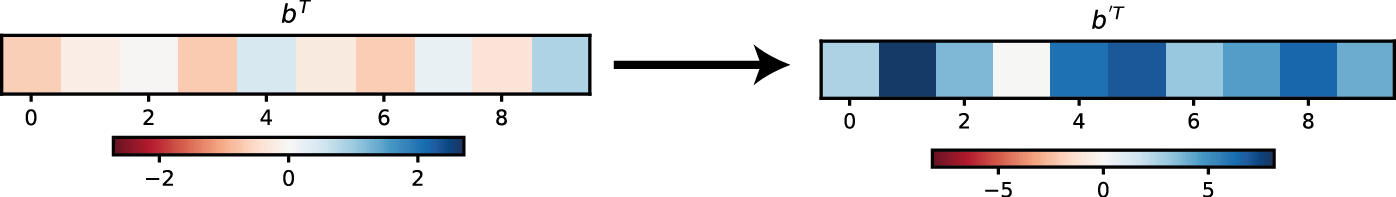
\includegraphics[width=0.9\linewidth]{sections/4_nn/imgs/bias.png}
   \end{center} \vspace{-10pt}
   
\end{frame}


% \begin{frame}{Transformation: Bias Integration}
% The last term can be \textbf{integrated} into an \textbf{updated bias}: 
% \begin{equation}
% \label{eq:bias_integration}
% \tilde{b}_i = b_i - \alpha\sum_{\{j |w_{ij} < 0\}}|{w}_{ij}| \in \mathbb{R}.
% \end{equation}

% The ne\textbf{w non-negative biases are transformed}:  
% \begin{equation}
% \label{eq:new_bias}
%     b^{'}_i = \tilde{b}_{i} + c \in \mathbb{R}_{+},
% \end{equation}
% with  \(c\in \mathbb{R}_{+}\) denotes \textbf{activation shifting point}
% \begin{equation}
%     c = \text{max}\{|\tilde{b}_0|, \ldots |\tilde{b}_{N}|\} \in \mathbb{R}_{+},
% \end{equation} 

% \begin{center}
%     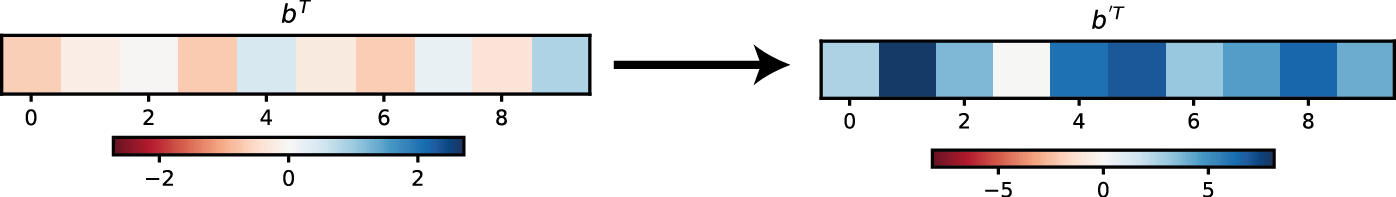
\includegraphics[width=0.9\linewidth]{sections/4_nn/imgs/bias.png}
% \end{center} \vspace{-10pt}

% \end{frame}

% The \textit{activation shifting point} is applied to the original activation to slide it into the input domain, preserving the variance of the original initialization scheme. To ensure that the network will function in a non-negative manner, the original activation function must operate within a closed interval with a non-negative output space, i.e., \(\phi^{(j)}(\bm{z}^{(j)}): \mathbb{R}^{N_{j}}\rightarrow [\phi^{(j)}_{min}, \phi^{(j)}_{max}]^{N_{j}}\), where \( 0 \leq \phi^{(j)}_{min} < \phi^{(j)}_{max} < \infty\), with the shifted activation calculated as:





\begin{frame}{Transformation: Activation Shifting Point}
The \textbf{activation shifting point} is applied \textbf{to the original activation},  \(\phi^{(j)}(\bm{z}^{(j)}): \mathbb{R}^{N_{j}}\rightarrow [\phi^{(j)}_{min}, \phi^{(j)}_{max}]^{N_{j}}\), where \( 0 \leq \phi^{(j)}_{min} < \phi^{(j)}_{max} < \infty\), to slide it into the input
domain, \textbf{leading to the same output as the original network}.
\begin{equation}
    \bm{y}^{(j)} = \phi^{(j)}_c(\bm{z}^{(j)})  = \phi^{(j)}(\bm{z}^{(j)} - \mathbbm{1}_{N_j} c^{(j)}) \in \mathbb{R}_{+}^{N_{j}}.
    \label{eq:nn_activation}
\end{equation}

\begin{center}
    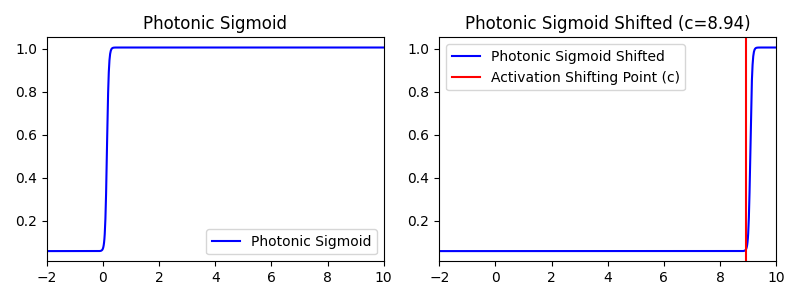
\includegraphics[width=0.8\linewidth]{sections/4_nn/imgs/sigmoid.png}
\end{center} 
\vspace{-10pt}
Typically, the \(\alpha^{(j+1)} \in \mathbb{R}_{+}\) of the next layer can be set to \(\alpha^{(j+1)} =
\phi^{(j)}_{max} = \text{max}(\mathcal{\bm{X}})\).      
\end{frame}

% \begin{frame}{Transformation: Non-negative Weights}

%   Similarly, the updated non-negative weights of the \(i\)-th neuron can be directly calculated as:
% \begin{equation}
%     \bm{w}'_{i} = |\bm{w}_i| \in \mathbb{R}_{+}^{M},
% \end{equation}
% % {\scriptsize where \(|\cdot|\) denotes the element-wise absolute value, i.e., \(w'_{ij} =
% % \{|w_{ij}|, j=0\ldots M\}\)}
% \begin{center}
%     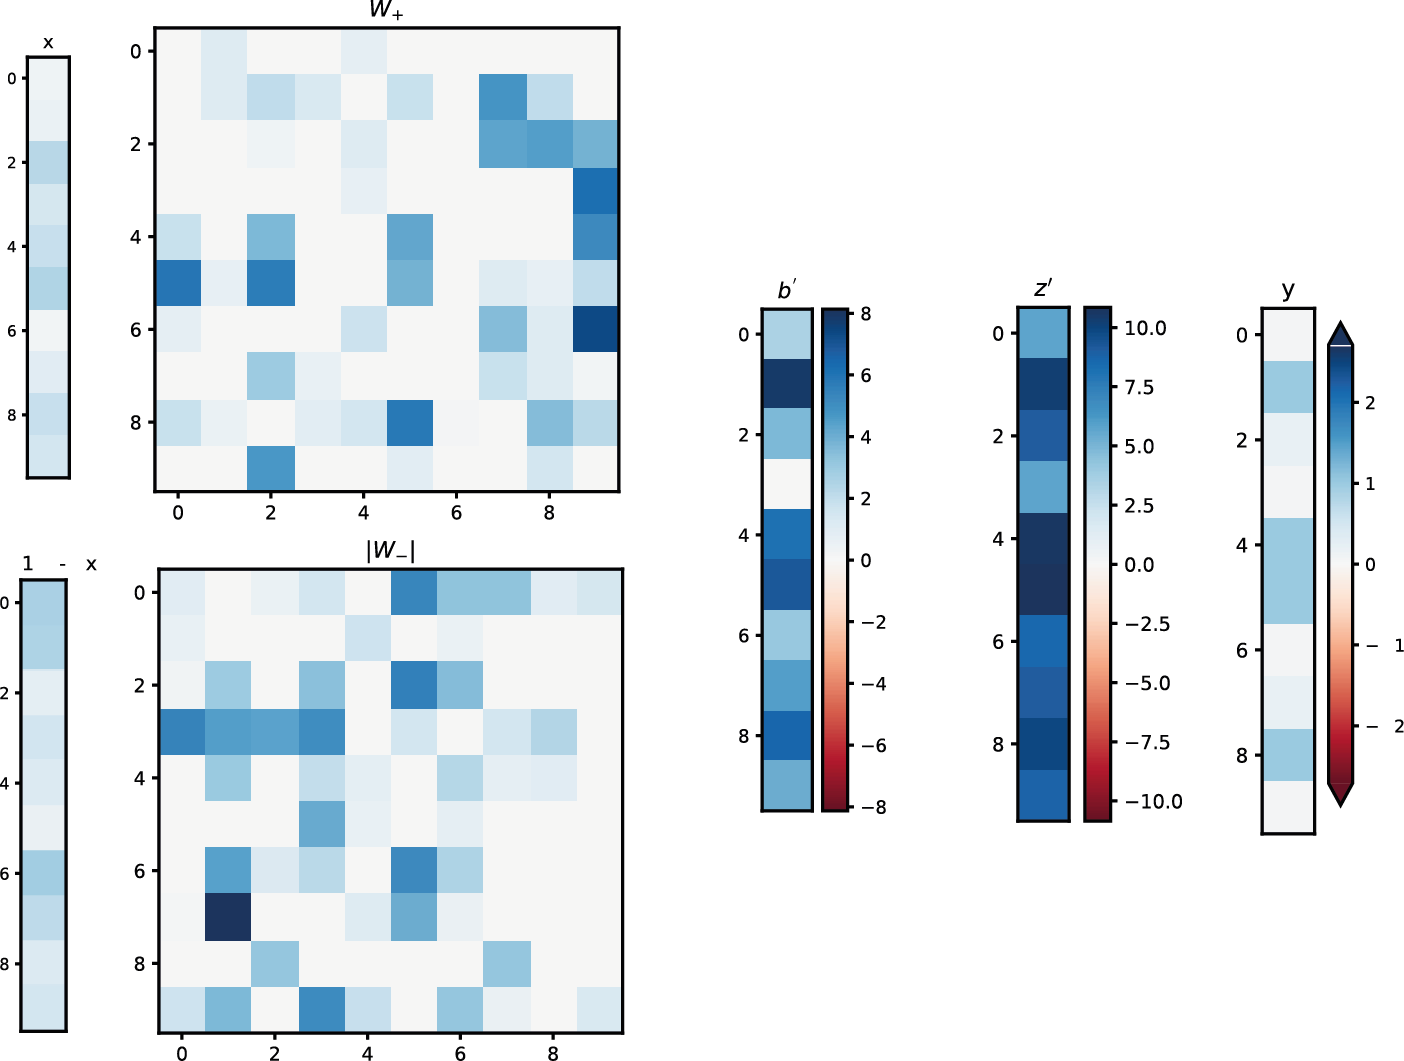
\includegraphics[width=0.7\linewidth]{sections/4_nn/imgs/overview_2.png}
% \end{center} 
    
% \end{frame}


% \begin{frame}{Non-negative Neuron}
% For \textbf{every linear neuron}, there is a \textbf{non-negative isomorphic} with the linear response provided as:
% \begin{equation}
%      z_i' = u_i'(\bm{x}')  =\sum_{j=1}^{M}|w_{ij}|x'_j + b'_i \in \mathbb{R}_+,
% \end{equation} and the output as: 
% \begin{equation}
%    y_i' = g_c(u_i'(\bm{x}')) \in \mathbb{R}_+,
% \end{equation} where:
% \begin{equation}
%     x'_j= 
%     \begin{cases}
%         \alpha - x_j & \text{if } w_{ij} <  0\\
%         x_j     & \text{otherwise}
%     \end{cases}.
% \end{equation}
% Then, the appropriate parameters \( b_i' \in \mathbb{R}_+ \) and \( \alpha \in \mathbb{R}_+ \), as well as the activation function \( g_c(\cdot): \mathbb{R} \rightarrow \mathbb{R}_+\) exist so that the neuron leads to the same response, i.e., \(y_i = y'_i\).
% \end{frame}

\begin{frame}{Post-initialization Remark}
	 Consider a linear layer followed by an activation function. defined by
   Equations~\ref{eq:linear} and~\ref{eq:activation}. Let the weights be
   initialized so that \(w_{ij} \sim \mathcal{D}(-a, a)\), and let the resulting
   activation distribution be denoted \(Y \sim \mathcal{A}(\mu, \sigma)\). 

    Given a post-initialization to non-negative weights \(\bm{W}^{'}=
    |\bm{W}|\), where \(\bm{W}_{+} + \bm{W}_{-} = |\bm{W}|\), there exist a
    corrective non-negative bias vector corrective \(\bm{b}^{'} \in
    \mathbb{R}_{+}^{N}\) and a shifted activation function \(\phi_c(\cdot):
    \mathbb{R}^{N} \rightarrow \mathbb{R}^{N}_{+}\) such that the new activation
    distribution \( Y^{'}\) satisfies \(Y^{'}\stackrel{d}{=}Y\). 
\end{frame}


\begin{frame}{Post-training Capability}
  \begin{figure}
\centering
    \begin{subfigure}{0.49\textwidth}
        \centering
        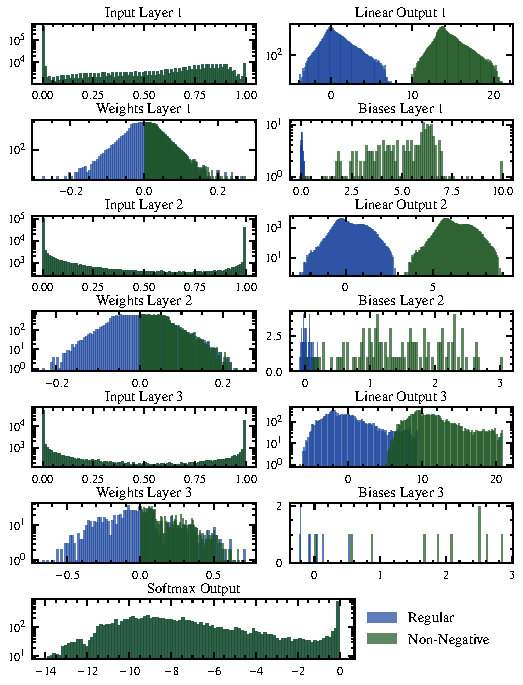
\includegraphics[width=0.8\textwidth]{sections/4_nn/imgs/transformation_plot.pdf}
    \end{subfigure}
    \hfill
    \begin{subfigure}{0.49\textwidth}
        \centering
        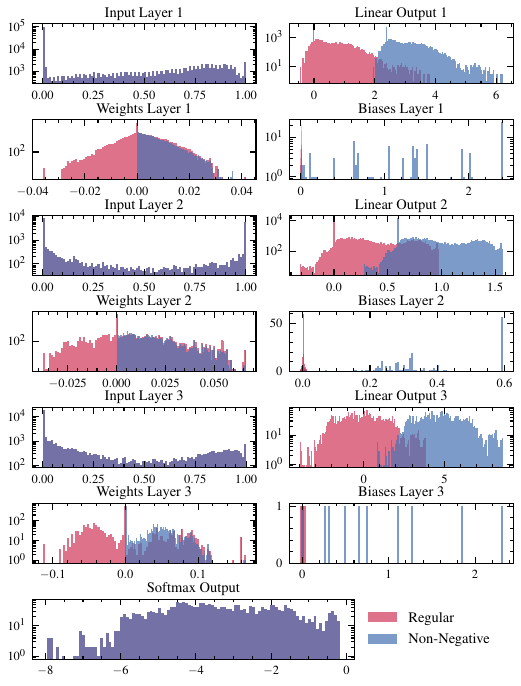
\includegraphics[width=0.8\textwidth]{sections/4_nn/imgs/variance_limited_range.png}
    \end{subfigure}
\end{figure}
\end{frame}


\begin{frame}{Generalibity}
  \begin{table}
    \begin{tabular}{l|c}
      Module                  & Covered \\
      \hline
      Recurrent Neuron        & $\checkmark$ \\
      Convolutional Neuron    & $\checkmark$ \\
      Padding                 & $\checkmark$ \\
      Negative Input          & $\checkmark$ \\
      Batch Normalization     & $\checkmark$ \\
      Residual Connection     & $\checkmark$ \\
    \end{tabular}
  \end{table}
\end{frame}

% \begin{frame}{Non-negative Stochastic Gradient Descent (NNSGD)}
% Transforming an already trained network to its non-negative isomorphic can be
%   \textbf{limiting in cases where continuing training is required.}
% \begin{equation}
% \small
% \theta_{\tau}^{(k)} = \theta_{\tau-1}^{(k)} +
% |\theta^{(k)}_{\tau-1}|\tanh{\left(-\eta_{in}\frac{\partial J}{\partial \theta^{(k)}_{\tau-1}} \right)} \eta_{out} \in \mathbb{R}^{+},
% \label{eq:3_m_abs}
% \end{equation}
% {\scriptsize where \(\eta_{in} \in \mathbb{R}^{+}\) is the inner and \(0 < \eta_{out} \leq
%   1\) the outer learning rate. } \\ \vspace{15pt}

% \textbf{NNSGD  modifies the additive update rule}, in which sign shifting is attributed
% during SGD optimization, by normalizing the gradients using the non-linear
% function \(\tanh: \mathbb{R} \rightarrow (-1, 1)\) and multiplying it by the
% absolute value of the parameter.  
% \end{frame}
\section{Evaluation Results}


\begin{frame}{Evaluation in Photonic Activations}
	\begin{table}
    \begin{center}
    \resizebox{0.85\linewidth}{!}{
    \begin{tabular}{l|l|lc|lc}
    % \toprule
      \multirow{2}{*}{Dataset} & \multirow{2}{*}{Architecture} & \multicolumn{2}{c|}{Photonic Sigmoid\footnote{\scriptsize P. Atanasijević, C. Pappas, et al,  Adaptive all-optical sigmoid activation functions for Photonic Neural Networks using Fabry-Perot laser diodes under optical injection, 2024 OFC }} & \multicolumn{2}{c}{Photonic Sinusoidal\footnote{\scriptsize N. Passalis, et al, Training Deep Photonic Convolutional Neural Networks With Sinusoidal Activations, 2021, IEEE TETCI}}\\
    \cline{3-6}
     && Proposed & \thead{Isomorphic\\Match} & Proposed & \thead{Isomorphic\\Match}\\
    \midrule
    MNIST & MLP & \(97.44\pm{0.08}\) & \checkmark & \(97.90\pm{0.10}\) & \checkmark\\ 
    MNIST & CNN & \(98.81\pm{0.14}\) & \checkmark & \(99.04\pm{0.07}\) & \checkmark \\
    FMNIST & MLP & \(85.64\pm{0.22}\) & \checkmark & \(86.30\pm{0.52}\) & \checkmark \\
    FMNIST & CNN & \(87.59\pm{0.47}\) & \checkmark & \(89.22\pm{0.18}\) & \checkmark \\
    CIFAR10 & MLP & \(37.08\pm{0.37}\) & \checkmark & \(39.48\pm{1.69}\) & \checkmark \\
    CIFAR10 & CNN & \(84.03\pm{0.69}\) & \checkmark & \(84.54\pm{0.28}\) & \checkmark \\
    Malimg\(^{*}\) & CNN & \(91.06\pm{4.56}\) & \checkmark & \(93.28\pm{4.30}\) & \checkmark \\
    Names & RNN & \(56.02\pm{0.70}\) & \checkmark & \(65.82\pm{0.90}\) & \checkmark \\
    FI2010\(^{\dagger}\) & RNN & \(0.1371\pm{0.0024}\) & \checkmark & \(0.1612\pm{0.0033}\)& \checkmark \\
    % \bottomrule
    \end{tabular}}
    \end{center}
    \vspace{-3pt}
    \scriptsize{\({*}\)F1 score, \({\dagger}\)Cohen's kappa score are reported, since the datasets are highly unbalanced}
\end{table}
\end{frame}

\begin{frame}{Evaluation on traditional (CNN Architectures)}
\begin{table}
  \begin{tabular}{lc|cc|cc|c}
    \multirow{2}{*}{\textbf{Architecture}} & \multirow{2}{*}{$\alpha$} &  \multicolumn{2}{c|}{\textbf{Original}} & \multicolumn{2}{c|}{\textbf{Isomorphic}} & \multirow{2}{*}{$ \mathbf{\leq0.5\%} $}\\
                 &          & \textbf{Acc@1} & \textbf{Acc@5} & \textbf{Acc@1} & \textbf{Acc@5} & \\
    \hline
    \textbf{AlexNet} & 25 & 56.52 & 79.06 & 56.36 & 79.10 & \checkmark\\
    \textbf{VGG11} & 25 & 69.02 & 88.62 & 68.95 & 88.59 & \checkmark\\
    \textbf{VGG13} & 40 & 69.93 & 89.25 & 69.83 & 89.28 & \checkmark\\
    \textbf{VGG16} & 100 & 71.59 & 90.38 & 71.59 & 90.40 & \checkmark\\
    \textbf{VGG19} & 100 & 72.37 & 90.87 & 72.39 & 90.90 & \checkmark\\
    \textbf{ResNet18} & 25 & 69.75 & 89.08 & 69.76 & 89.08 & \checkmark\\
    \textbf{ResNet34} & 25 & 73.31 & 91.42 & 73.29 & 91.42 & \checkmark\\
    \textbf{ResNet50} & 100 & 80.85 & 95.43 & 80.35 & 95.13 & \checkmark\\
    \textbf{ResNet101} & 100 & 81.88 & 95.78 & 81.67 & 95.66 & \checkmark\\
    \textbf{ResNet152} & 100 & 82.28 & 96.00 & 82.34 & 95.34 & \checkmark\\
  \end{tabular}
\end{table}
\end{frame}

% \begin{frame}{Post-training Variance Study}
%   \begin{figure}
%     \centering
%     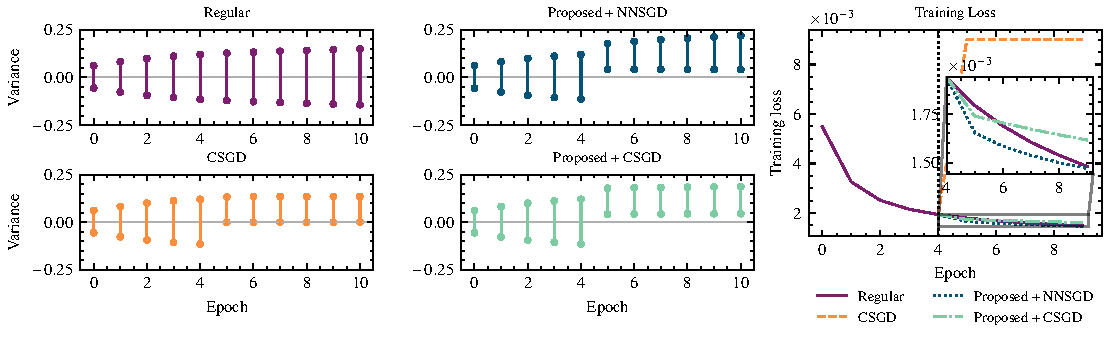
\includegraphics[width=\linewidth]{sections/4_nn/imgs/variance_fmnist_photonic_sigmoid.pdf}
%     % \vspace{-25pt}
%     \caption{Depicts the variance of classification layer in photonic sigmoid architecture applied on FMNIST dataset. Additionally, in the right subfigure, the loss during the training is presented. Networks are pre-trained for 5 epochs with SGD and then they are either transformed with the proposed method or clipping is applied directly. The figure in the top left shows the variance of the regular training. }
%     \label{fig:fmnist_variance}
%     % \vspace{-15pt}
% \end{figure}
% \end{frame}


% \begin{frame}{Non-negative Post-training (MLPs)}
%    \begin{table}[]
%     \centering
%      \caption{Non-negative post training after transformation using MLPs}  
%       \label{tab:3_half_fcnn}
%     \begin{tabular}{l|ll|l}
%          % \toprule
%          Dataset  & \thead{Regular\\+ CSGD} & \thead{Proposed\\+ CSGD} &  \thead{Proposed\\+ NNSGD}  \\
%          \midrule
%          \multicolumn{4}{c}{Photonic Sigmoid}\\
%          \midrule
%          MNIST  & \(11.00\pm{0.00}\) & \(\bm{97.31\pm{0.90}}\) & \(\underline{\bm{97.40\pm{0.06}}}\) \\
%          FMNIST & \(10.00\pm{0.00}\) & \(\bm{84.77\pm{0.21}}\) & \(\underline{\bm{85.01\pm{0.12}}}\) \\
%          CIFAR10 & \(10.00\pm{0.00}\) & \(\bm{36.34\pm{0.37}}\) & \(\underline{\bm{36.81\pm{0.33}}}\)\\
%          \midrule
%          \multicolumn{4}{c}{Photonic Sinusoidal}\\
%          \midrule
%          MNIST  &  \(09.74\pm{0.00}\)  & \(\bm{97.85\pm{0.10}}\) & \(\underline{\bm{97.86\pm{0.07}}}\) \\
%          FMNIST  & \(10.00\pm{0.00}\) & \(\bm{86.62\pm{0.09}}\) & \(\underline{\bm{86.95\pm{0.17}}}\)\\
%          CIFAR10 & \(10.00\pm{0.00}\) & \(\bm{40.96\pm{0.30}}\) & \(\underline{\bm{41.19\pm{0.38}}}\)\\
%          % \bottomrule
%     \end{tabular}
% \end{table}
% \end{frame}

% \begin{frame}{Non-negative Post-training (CNNs \& RNNs)}
% 	\begin{table}
% \caption{Non-negative post training after transformation using CNNs and RNNs \label{tab:half}}
%     \begin{center}
%     \resizebox{\linewidth}{!}{
%     \begin{tabular}{l|ll|ll}
%     % \toprule
%         Config.& \multicolumn{2}{|c|}{Photonic Sigmoid}  & \multicolumn{2}{|c}{Photonic Sinusoidal}\\
%         \midrule
%         Method  & \thead{Proposed\\+ CSGD} & \thead{Proposed\\+ NNSGD} & \thead{Proposed\\+ CSGD} & \thead{Proposed\\+ NNSGD}  \\
%         \midrule
%         MNIST & \(96.85\pm{0.96}\) & \(\bm{97.60\pm{1.83}}\) & \(98.58\pm{0.12}\) & \(\bm{99.04\pm{0.07}}\) \\
%         FMNIST & \(83.90\pm{0.46}\) & \(\bm{84.87\pm{0.33}}\) & \(87.59\pm{0.20}\) &  \(\bm{87.63\pm{0.19}}\) \\
%         CIFAR10 & \(74.30\pm{0.22}\) & \(\bm{77.39\pm{0.56}}\) & \(77.30\pm{0.73}\) & \(\bm{79.95\pm{0.21}}\) \\
%         Malimg\(^{*}\) & \(93.53\pm{2.76}\) & \(\bm{96.60\pm{0.78}}\) & \(92.18\pm{4.52}\) & \(\bm{93.53\pm{4.30}}\) \\
%         \midrule
%         Names & \(53.94\pm{1.44}\) & \(\bm{58.37\pm{1.05}}\) &  \(66.64\pm{0.83}\) & \(\bm{67.14\pm{0.54}}\) \\
%         FI2010\(^{\dagger}\) & \(0.1050\pm{0.0070}\) & \(\bm{0.1220\pm{0.0022}}\) & \(0.1434\pm{0.0014}\)  & \(\bm{0.1840\pm{0.0018}}\) \\
%         % \bottomrule
%     \end{tabular}}
%      \end{center}
%      \vspace{-3pt}
%     \scriptsize{\({*}\)F1 score, \({\dagger}\)Cohen's kappa score are reported, since the datasets are highly unbalanced}
%     \vspace{-10pt}
% \end{table}
% \end{frame}



% \begin{frame}{Non-negative Training from Scratch (MLPs)}
% 	\begin{table}[]
%     \centering
%          \caption{Non-negative training from scratch in MLPs}  
%       \label{tab:full_fcnn}
%     \resizebox{\linewidth}{!}{
%     \begin{tabular}{l|ll|ll}
%          \toprule
%          Dataset  & \thead{Exp. Initialization\\+ CSGD} & \thead{Proposed\\+ CSGD} & \thead{Exp. Initialization\\+ NNSGD} & \thead{Proposed\\+ NNSGD}  \\
%          \midrule
%          \multicolumn{5}{c}{Photonic Sigmoid}\\
%          \midrule
%          MNIST & \(11.35\pm{0.00}\) &\(\bm{92.52\pm{0.52}}\) & \(11.35\pm{0.00}\) & \(\underline{\bm{93.34\pm{1.11}}}\) \\
%          FMNIST & \(10.00\pm{0.00}\) &\(\bm{82.31\pm{1.29}}\) & \(10.00\pm{0.00}\) & \(\underline{\bm{84.09\pm{0.56}}}\)\\
%          CIFAR10 & \(10.00\pm{0.00}\) &\(\bm{37.25\pm{1.57}}\)  & \(10.00\pm{0.00}\) & \(\underline{\bm{37.61\pm{1.76}}}\)\\
%          \midrule
%          \multicolumn{5}{c}{Photonic Sinusoidal}\\
%          \midrule
%          MNIST  & \(86.36\pm{1.39}\) &\(\bm{92.51\pm{0.78}}\) & \(35.31\pm{6.11}\) & \(\underline{\bm{94.14\pm{0.90}}}\)\\
%          FMNIST & \(68.95\pm{3.71}\) &\(\bm{82.91\pm{0.55}}\)   & \(9.97\pm{0.02}\) & \(\underline{\bm{83.57\pm{0.26}}}\)\\
%          CIFAR10 &  \(10.00\pm{0.00}\) &\(\bm{34.96\pm{2.44}}\) & \(10.00\pm{0.00}\)  & \(\underline{\bm{35.41\pm{1.43}}}\)\\ 
%          \bottomrule
%     \end{tabular}}
%   \end{table}
%   \end{frame}

% \begin{frame}{Non-negative Training from Scratch (CNNs \& RNNs)}
%   \begin{table}[]
%    \caption{Non-negative training from scratch in CNNs and RNNs \label{tab:full}} 
%     \begin{center}
%     \resizebox{\linewidth}{!}{
%     \begin{tabular}{l|ll|ll}
%     \toprule
%         Config.& \multicolumn{2}{|c|}{Photonic Sigmoid}  & \multicolumn{2}{|c}{Photonic Sinusoidal}\\
%         \midrule
%         Method  & \thead{Proposed\\+ CSGD} & \thead{Proposed\\+ NNSGD} & \thead{Proposed\\+ CSGD} & \thead{Proposed\\+ NNSGD}  \\
%         \midrule
%         MNIST & \(97.69\pm{0.20}\) & \(\bm{98.14\pm{0.23}}\) & \(98.54\pm{0.14}\) & \(\bm{98.71\pm{0.05}}\) \\
%         FMNIST & \(83.81\pm{0.85}\) & \(\bm{83.87\pm{0.19}}\) & \(87.77\pm{0.36}\) & \(\bm{87.86\pm{0.36}}\)\\
%         CIFAR10 & \(71.61\pm{1.04}\) & \(\bm{72.16\pm{0.54}}\) & \(69.87\pm{1.73}\) & \(\bm{75.16\pm{1.83}}\)\\
%         Malimg\(^{*}\) & \(91.47\pm{4.37}\) & \(\bm{91.98\pm{4.00}}\) & \(96.53\pm{0.42}\) & \(\bm{97.26\pm{0.31}}\) \\
%         \midrule
%         Names & \(54.00\pm{2.13}\) & \(\bm{56.68\pm{1.11}}\) & \(64.17\pm{0.14}\) & \(\bm{68.70\pm{0.78}}\) \\
%         FI2010\(^{\dagger}\) & \(0.1338\pm{0.0045}\) & \(\bm{0.1498\pm{0.0112}}\) & \(0.1732\pm{0.0175}\) & \(\bm{0.1789\pm{0.0102}}\)\\
%         \bottomrule
%     \end{tabular}}
%      \end{center}
%      \vspace{-3pt}
%     \scriptsize{\({*}\)F1 score, \({\dagger}\)Cohen's kappa score are reported, since the datasets are highly unbalanced.}
% \end{table}
% \end{frame}

% \begin{frame}{Publication}
% \begin{itemize}
%     \item Main Journal Submission
%     \begin{itemize}
%         \item {\scriptsize \textbf{Kirtas, M.}, Passalis, N., Pleros, N., Tefas, A., 2024. \href{https://arxiv.org/abs/2310.01084}{Non-Negative Isomorphic Neural Networks for Efficient Accelerators.} \textbf{Submitted}}
%     \end{itemize}
%     \item Main Conferences Publications 
%         \begin{itemize}
%         \item {\scriptsize \textbf{Kirtas, M.}, Tsampazis, K., Avramelou, L., Passalis, N. and Tefas, A., 2023, September. \href{https://link.springer.com/chapter/10.1007/978-3-031-74627-7_35}{Using Part-based Representations for Explainable Deep Reinforcement Learning.} In Joint European Conference on Machine Learning and Knowledge Discovery in Databases}
%     \end{itemize}
% \end{itemize}
% \end{frame}

% \section{Multiplicative Updates for DL Training}

\begin{frame}{Thesis Contribution}
  Even though \textbf{multiplicative updates have several interesting properties}
  for neural networks and their hardware integration, \textbf{they are merely studied in
  the literature}.
  
  \begin{itemize}
    \item An \textbf{generic framework for alternative update rules}, allowing moderate
      the update rules for all well known optimization methods
    \item A \textbf{novel multiplicative update rule} that \textbf{accelerates} convergence and\textbf{ robustness} of training
    \item A \textbf{hybrid multiplicative-additive} update that \textbf{overcomes the limitations} of multiplicative updates
  \end{itemize}	
\end{frame}

\begin{frame}{Generic Optimization Framework for Alternative Updates}
\begin{algorithm}[H]
  \SetKwData{Left}{left}\SetKwData{This}{this}
  \SetKwData{Up}{up}\SetKwFunction{Union}{Union}
  \SetKwFunction{FindCompress}{FindCompress}
  \Begin{
      \While{\(t=1\) to \(T\) }{
        \(g_t = \nabla_{\theta}f_t(\theta_{t-1}) \) Gradients \\
        \(m_t = \phi_{t}(g_1,\ldots, g_t):\mathbb{R}^{t} \rightarrow \mathbb{R}
        \) Momentum \\
        \(l_t = \psi_{t}(g_1,\ldots, g_t): \mathbb{R}^{t} \rightarrow \mathbb{R}^{t}\) Adaptive Learning Rate \\
        \(\Delta\theta_t = \xi(\theta_{t-1}, m_t, l_t, \eta): \mathbb{R}^{t}
        \rightarrow \mathbb{R}\) Update Rule \\
      }
    }
    \caption{Generic Optimization Framework for Alternative Updates (GOFAU) \label{alg:optim}}    
\end{algorithm}
\end{frame}

\begin{frame}{Additive Optimization Methods}  
	\begin{table}
    \renewcommand{\arraystretch}{3.5}
    \begin{tabularx}{\linewidth}{l|c|c|c|c}
      & \textbf{SGD} & \textbf{Adagrad} & \textbf{Adam} & \textbf{RMSprop} \\
      \hline
      \(\phi_{t}(\cdot)\) & \(g_t\) & \(g_t\) &
                                                          \(\frac{(1-\beta_1)\sum_{i=1}^t\beta_1^{t-i}g_i}{1-\beta_1^t}\)
                             &  \(g_t\) \\
      \hline
      \(\psi_{t}(\cdot)\)    &  1  & \( \left( \sum_{i=1}^{t}g_i^2 \right)^{-1/2}\) &
                                                                 \(\sqrt{\frac{1-\beta_2^t}{(1-\beta_2)\sum_{i=1}^{t}\beta_2^{t-i}g_i^2}}\)
                                                          &
                                                            \(\sqrt{\frac{1-\beta_2^t}{(1-\beta_2)\sum_{i=1}^{t}\beta_2^{t-i}g_i^2}}\)\\
      \hline     
      \(\xi(\cdot)\) & \multicolumn{4}{c}{\cellcolor{blue!25}\(\eta m_t l_t\)}
    \end{tabularx}
  \end{table}
\end{frame}

\begin{frame}{Limitation of Additive Update}    
	
    \begin{equation*}
    \theta_t = \theta_{t-1} - \eta m_t l_t
  \end{equation*}
  
  \begin{itemize}
    \item \textbf{Depends on the gradient values} and the \textbf{learning rate}
    \item Extremely \textbf{sensitive to magnitude} of parameters
    \item Training difficulties when parameters are far from local or global
      minimum
    \item This exists profoundly when the \textbf{initialization is bad}
    \item Difficulties with default learning rate values
  \end{itemize}

\end{frame}

\begin{frame}{Proposed Multiplicative Update}
	\begin{table}
    \renewcommand{\arraystretch}{3.5}
    \begin{tabularx}{\linewidth}{l|c|c|c|c}
      & \textbf{SGD} & \textbf{Adagrad} & \textbf{Adam} & \textbf{RMSprop} \\
      \hline
      \(\phi_{t}(\cdot)\) & \(g_t\) & \(g_t\) &
                                                          \(\frac{(1-\beta_1)\sum_{i=1}^t\beta_1^{t-i}g_i}{1-\beta_1^t}\)
                                                          &  \(g_t\) \\ \hline
      \(\psi_{t}(\cdot)\)   & 1  & \( \left( \sum_{i=1}^{t}g_i^2 \right)^{-1/2}\) &
                                                                 \(\sqrt{\frac{1-\beta_2^t}{(1-\beta_2)\sum_{i=1}^{t}\beta_2^{t-i}g_i^2}}\)
                                                          &
                                                            \(\sqrt{\frac{1-\beta_2^t}{(1-\beta_2)\sum_{i=1}^{t}\beta_2^{t-i}g_i^2}}\)\\ \hline
      \(\xi(\cdot)\) & \multicolumn{4}{c}{\cellcolor{blue!25} \(|\theta_{t-1}|\tanh{\left(\eta_{in} m_t l_t \right)}\eta_{out}\)}

    \end{tabularx}
  \end{table}
\end{frame}

\begin{frame}{Benefits of Multiplicative Update Rule}
  \tikzstyle{na} = [baseline=-.5ex]
  
  \begin{itemize}[<+-| alert@+>]
  \item Normalize gradient 
    \tikz[na]\node [coordinate] (nCPP) {};
  \item Proportionally scales
    \tikz[na]\node [coordinate] (tps) {};
  \end{itemize}
  
	\begin{equation}
    \theta_{t} = \theta_{t-1} -
    \tikz[baseline]{\node[fill=blue!20,anchor=base] (mps) {$|\theta_{t-1}|$} ;}
    \tikz[baseline]{\node[fill=blue!20,anchor=base] (tL) {$\tanh$};}
    \tikz[baseline]{\node[fill=blue!20,anchor=base] (mml) {{$\left(\eta_{in} m_t l_t \right)$}};}
    \tikz[baseline]{\node[fill=blue!20,anchor=base] (mtu) {$\eta_{out}$};}
  \end{equation}

  \begin{tikzpicture}[overlay]
    \path[->]<1-> (nCPP) edge [bend left] (tL);
    \path[->]<2-> (tps) edge [bend left] (mps);
    \path[->]<3-> (bml) edge [bend right] (mml);
    \path[->]<4-> (btu) edge [bend right] (mtu);

        % \path[->]<2-> (nL) edge [bend left] (tL);
        % \path[->]<3-> (nPPP) edge [out=0, in=0] (tPPP);
        % \path[->]<4-> (nPP) edge [out=0, in=-90] (tPP);
  \end{tikzpicture}

  \begin{itemize}[<+-| alert@+>]
  \item Measures the scaling
    \tikz[na]\node [coordinate] (bml) {};
  \item Proportionally thresholds the update \tikz[na]\node [coordinate] (btu) {};
    \begin{itemize}
    \item \(\left[-\eta_{out}|\theta_{t-1}|, \eta_{out}|\theta_{t-1}|\right]\)
    \end{itemize}
  \item Preserves the sign of parameter
  \begin{itemize}
      \item \(\theta_{t}\theta_{t-1} \geq 0\)
    \end{itemize}
  \end{itemize}

\end{frame}

% \begin{frame}
% \tikzstyle{na} = [baseline=-.5ex]

% \begin{itemize}[<+-| alert@+>]
%     \item Class Prior Probability
%         \tikz[na]\node [coordinate] (nCPP) {};
%     \item Likelihood
%         \tikz[na]\node [coordinate] (nL) {};
% \end{itemize}

% \begin{equation*}
% \frac{
% \tikz[baseline]{\node[fill=blue!20,anchor=base] (tL) {$p(D|\theta)$};}
% \tikz[baseline]{\node[fill=red!20,anchor=base] (tCPP) {$p(\theta)$};}
% }
% {
% \tikz[baseline]{\node[fill=green!20,anchor=base] (tPPP) {$p(D)$};}
% }
% =
% \tikz[baseline]{\node[fill=yellow!20,anchor=base] (tPP) {$p(\theta | D)$};}
% \end{equation*}
% \begin{itemize}[<+-| alert@+>]
%     \item Predictor Prior Probability
%         \tikz[na]\node [coordinate] (nPPP) {};
%     \item Posterior probability
%         \tikz[na] \node[coordinate] (nPP) {};
% \end{itemize}

% \begin{tikzpicture}[overlay]
%         \path[->]<1-> (nCPP) edge [bend left] (tCPP);
%         \path[->]<2-> (nL) edge [bend left] (tL);
%         \path[->]<3-> (nPPP) edge [out=0, in=0] (tPPP);
%         \path[->]<4-> (nPP) edge [out=0, in=-90] (tPP);
% \end{tikzpicture}
% \end{frame}

\begin{frame}{Proposed Hybrid Update}
	\begin{table}
    \renewcommand{\arraystretch}{3.5}
    \begin{tabularx}{\linewidth}{l|c|c|c|c}
      & \textbf{SGD} & \textbf{Adagrad} & \textbf{Adam} & \textbf{RMSprop} \\
      \hline
      \(\phi_{t}(\cdot)\) & \(g_t\) & \(g_t\) &
                                                          \(\frac{(1-\beta_1)\sum_{i=1}^t\beta_1^{t-i}g_i}{1-\beta_1^t}\)
                                                          &  \(g_t\) \\ \hline
      \(\psi_{t}(\cdot)\)    & 1  & \( \left( \sum_{i=1}^{t}g_i^2 \right)^{-1/2}\) &
                                                                 \(\sqrt{\frac{1-\beta_2^t}{(1-\beta_2)\sum_{i=1}^{t}\bConvexeta_2^{t-i}g_i^2}}\)
                                                          &
                                                            \(\sqrt{\frac{1-\beta_2^t}{(1-\beta_2)\sum_{i=1}^{t}\beta_2^{t-i}g_i^2}}\)\\ \hline
      \(\xi(\cdot)\) & \multicolumn{4}{c}{\cellcolor{blue!25} \(\gamma\left(|\theta_{t-1}|\tanh{\left(\eta_{in} m_t l_t \right)}\eta_{out}\right) + (1-\gamma) \left(\eta m_t l_t\right)\)}
                                                                                                                                              
    \end{tabularx}
  \end{table}
\end{frame}

\begin{frame}{Proposed Hybrid Update}
  \begin{itemize}[<+-| alert@+>]
  \item Additive: Overcomes sign limitation \tikz[na]\node [coordinate] (tos) {};
  \item Acceleration and robustness  \tikz[na]\node [coordinate] (tar) {};
  \end{itemize}
  
	\begin{equation}
    \theta_{t} = \theta_{t-1} -
    \tikz[baseline]{\node[fill=blue!20,anchor=base] (mwra) { $\gamma$} ;}
    \tikz[baseline]{\node[fill=blue!20,anchor=base] (mar) { $\left(|\theta_{t-1}|\tanh{\left(\eta_{in} m_t l_t \right)}\eta_{out}\right) $} ;}
    +
    \tikz[baseline]{\node[fill=blue!20,anchor=base] (mwrb) { $(1-\gamma) $} ;}
    \tikz[baseline]{\node[fill=blue!20,anchor=base] (mos) { $ \left(\eta m_t l_t\right) $} ;}
  \end{equation}
  
  \begin{itemize}[<+-| alert@+>]
    \item Weights relative \tikz[na]\node [coordinate] (bwra) {}; contribution \tikz[na]\node [coordinate] (bwrb) {};
    \end{itemize}

    \begin{tikzpicture}[overlay]
      \path[->]<1-> (tos) edge [bend left] (mos);
      \path[->]<2-> (tar) edge [bend left] (mar);
      \path[->]<3-> (bwra) edge [bend] (mwra);
      \path[->]<3-> (bwrb) edge [bend right] (mwrb);
    \end{tikzpicture}
\end{frame}

\begin{frame}{Experimental Evaluation: An Example}
	\begin{figure}
    \centering
    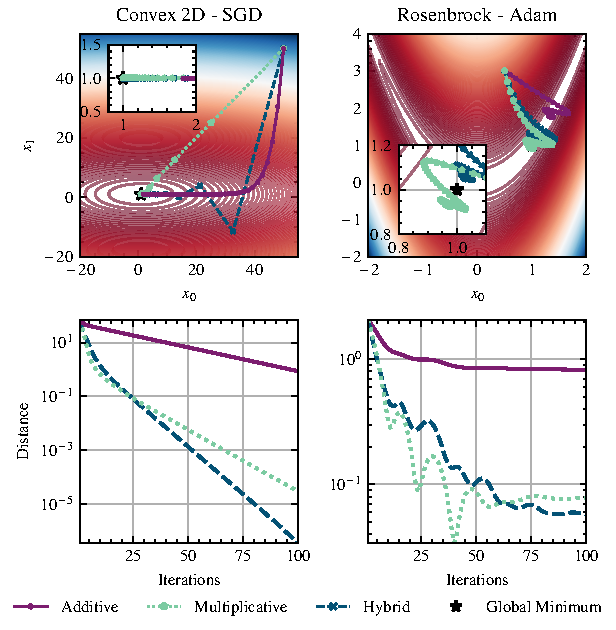
\includegraphics[width=0.75\linewidth]{./sections/5_mult/imgs/selection_convex.pdf}
    % \caption{The top Figures demonstrate the optimization process for Convex 2D
    %   and Rosenbrock tasks alternative updates for SGD and Adam optimizers,
    %   respectively. The bottom Figures report the Euclidean distance between the
    %   parameters and the actual global minimum. }
    \label{fig:convex_opt}
\end{figure}
\end{frame}


% \begin{frame}{Experimental Results}
% 	\begin{table}[]
%     \centering
%      \caption{Distance from global minimum after 100 iterations using the best training configuration}
%     \label{tab:tune_convex}
%     \resizebox{0.8\linewidth}{!}{\begin{tabular}{l|c|c|c}
%          \toprule
%          Optimizer & \mythead{\normalfont Baseline\\\normalfont(Additive)} & \mythead{\textbf{GOFAU}\\\textbf{(Multiplicative)}} & \mythead{\textbf{GOFAU}\\\textbf{(Hybrid)}} \\
%          \midrule
%          \multicolumn{4}{c}{\textbf{Convex 2D} \textit{(69.26)}}\\ \midrule
%          SGD & \(8.61\times10^{-1}\) & \(2.92\times10^{-5}\) & \(\bm{3.57\times10^{-7}}\)  \\
%          Adagrad & \(5.80\times10^{-4}\) & \(1.35\times10^{-4}\) & \(\underline{\bm{1.68\times10^{-7}}}\) \\
%          Adam & \(3.75\times10^{-2}\) & \(7.44\times10^{-3}\) & \(\bm{4.47\times10^{-3}}\)  \\
%          RMSProp & \(1.82\times10^{-5}\) & \(7.58\times10^{-6}\) & \(\underline{\bm{1.68\times10^{-7}}}\)  \\ \midrule
%          \multicolumn{4}{c}{\textbf{Rosenbrock} \textit{(2.06)}}\\ \midrule
%          SGD & \(1.38 \times 10^{0}\) & \(7.70\times10^{-2}\) & \(\bm{2.04\times10^{-2}}\) \\
%          Adagrad & \(4.60 \times 10^{-1}\) & \(1.88\times10^{-1}\) &  \(\underline{\bm{1.26\times10^{-2}}}\) \\
%          Adam & \(8.24\times 10^{-1}\) & \(7.84\times10^{-2}\) & \(\bm{5.73\times10^{-2}}\) \\
%          RMSProp & \(4.58\times10^{-1}\) & \(1.85\times10^{-1}\)  & \(\bm{5.06\times10^{-2}}\)  \\
%         \bottomrule
%     \end{tabular}}
% \end{table}
% \end{frame}



% \begin{frame}{Experimental Evaluation: Robustness}
% 	\begin{table*}
%     \centering
%     \caption{Evaluation of optimizers on 100 randomly drawn configurations. The relative Euclidean distance the parameters and the actual global minimum is reported }
%     \label{tab:convex_res}
%     \resizebox{\linewidth}{!}{\begin{tabular}{l|l|l|l}
%          \toprule
%          Optimizer & \mythead{\normalfont Baseline\\\normalfont(Additive)} & \mythead{\textbf{GOFAU}\\\textbf{(Multiplicative)}} & \mythead{\textbf{GOFAU}\\\textbf{(Hybrid)}} \\
%          \midrule
%          \multicolumn{4}{c}{\textbf{Convex 2D}}\\ \midrule
%          SGD & \(1.48\times10^{-2}\pm{8.06\times10^{-3}}\) & \(1.82\times10^{-3}\pm{5.17\times10^{-3}}\) & \(\bm{8.37\times10^{-4} \pm{2.35\times10^{-3}}}\)  \\
%          Adagrad & \(7.61\times10^{-5}\pm{1.67\times10^{-4}}\) & \(2.30\times10^{-3}\pm{7.17\times10^{-3}}\) & \(\underline{\bm{1.79\times10^{-9} \pm{1.34\times10^{-9}}}}\) \\
%          Adam & \(4.28\times10^{-3}\pm{4.28\times10^{-3}}\) & \(3.95\times10^{-3}\pm{4.88\times10^{-3}}\) & \(\bm{1.26\times10^{-3}\pm{1.45\times10^{-3}}}\)  \\
%          RMSProp & \(8.26\times10^{-6}\pm{2.33\times10^{-5}}\) & \(2.24\times10^{-3}\pm{2.24\times10^{-3}}\) & \(\bm{2.01\times10^{-8}\pm{9.58\times10^{-8}}}\)  \\ \midrule
%          \multicolumn{4}{c}{\textbf{Rosenbrock}}\\ \midrule
%          SGD & \(5.88\times10^{-1}\pm{2.19\times10^{-1}}\) & \(1.75\times10^{-1}\pm{2.36\times10^{-1}}\) & \(\underline{\bm{7.42\times10^{-2}\pm{1.53\times10^{-1}}}}\) \\
%          Adagrad & \(3.53\times10^{-1}\pm{3.59\times10^{-1}}\) & \(2.03\times10^{-1}\pm{2.13\times10^{-1}}\) &  \(\bm{1.98\times10^{-1}\pm{2.68\times10^{-1}}}\) \\
%          Adam & \(4.12\times10^{-1}\pm{1.69\times10^{-1}}\) & \(1.68\times10^{-1}\pm{2.55\times10^{-1}}\) & \(\bm{1.48\times10^{-1}\pm{1.58\times10^{-1}}}\) \\
%          RMSProp & \(3.16\times10^{-1}\pm{3.08\times10^{-1}}\) & \(1.43\times10^{-1}\pm{1.67\times10^{-1}}\)  & \(\bm{2.01\times10^{-1}\pm{2.51\times10^{-1}}}\)  \\
%         \bottomrule
%     \end{tabular}}
% \end{table*}
% \end{frame}

\begin{frame}{Experimental Evaluation: Robustness}
	\begin{figure}
    \centering
    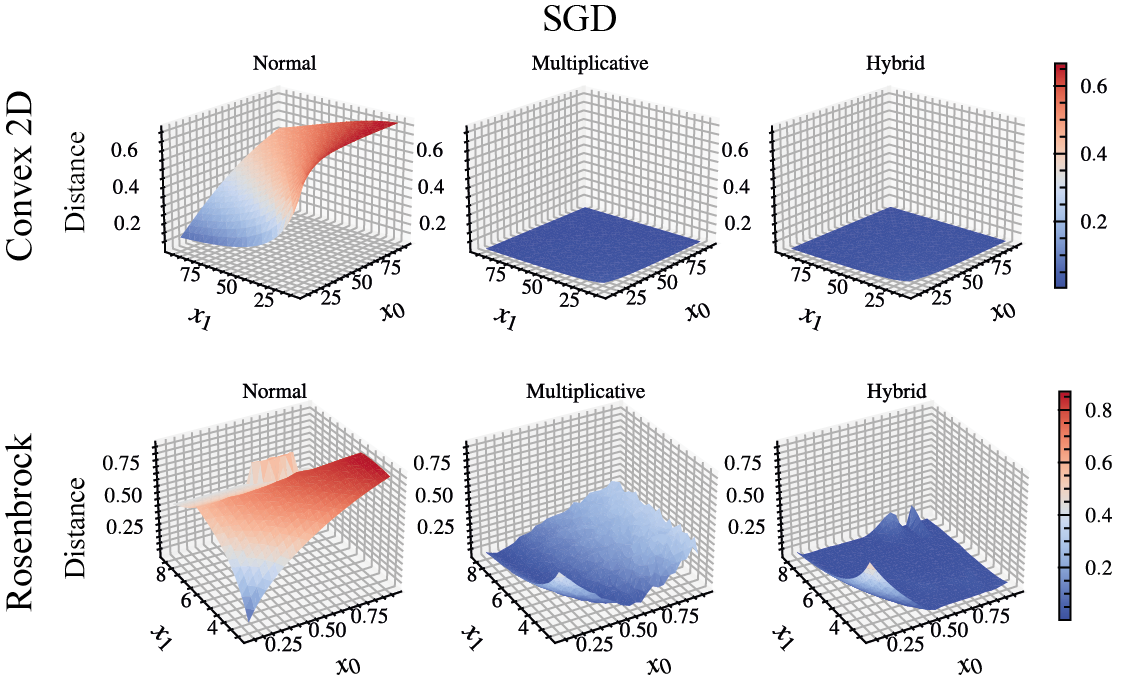
\includegraphics[width=\textwidth]{./sections/5_mult/imgs/surface_plot_v2.png}
    \caption{Distance from global minimum of the evaluated update rules applying
      SGD optimization methods in two optimization tasks. }
    \label{fig:surface_plot}
\end{figure}
\end{frame}


% \begin{frame}{CIFAR100 - ResNet18}
% 	\begin{figure}
%     \centering
%     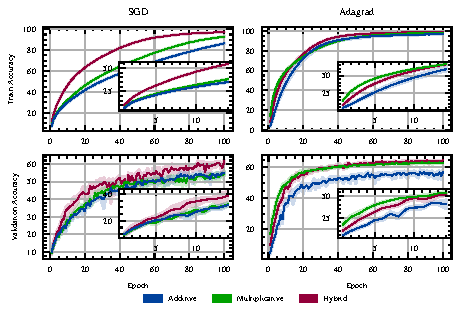
\includegraphics[width=\linewidth]{./sections/5_mult/imgs/230309_cifar100_resnet18.pdf} 
%     % \caption{Training and validation accuracy during training applying ResNet18
%     %   architecture on CIFAR100 dataset using default configurations for both
%     %   task and optimizers }
%     \label{fig:cifar100}
%   \end{figure}
% \end{frame}

% \begin{frame}{Tiny ImageNet - ResNet18}
%   \begin{figure}[t]{\linewidth}
%         \centering
%         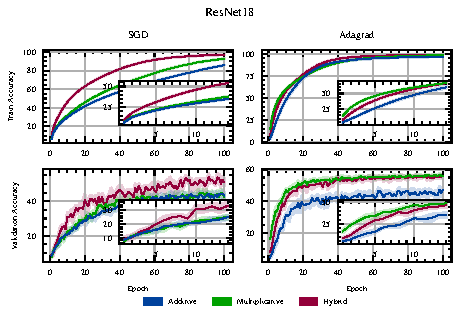
\includegraphics[width=\linewidth]{./sections/5_mult/imgs/230313_tiny_imagenet_resnet18.pdf}
%       %   \caption{Training and validation accuracy during training on Tiny ImageNet
%       % dataset using default configurations for both task and optimizers}
%     \end{figure}
% \end{frame}

\begin{frame}{Experimental Evaluation: Tiny ImageNet - ResNet18}
      \begin{figure}[t]{\linewidth}
        \centering
        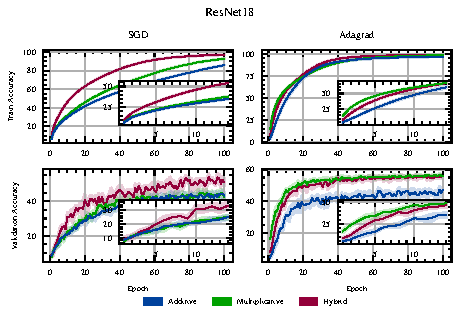
\includegraphics[width=\linewidth]{./sections/5_mult/imgs/230313_tiny_imagenet_resnet18.pdf}
      %   \caption{Training and validation accuracy during training on Tiny ImageNet
      % dataset using default configurations for both task and optimizers}
    \end{figure}
\end{frame}

\begin{frame}{Experimental Evaluation: CIFAR100 - ResNet18}
    \begin{table}
  \centering
    \begin{tabular}{l|ccc}
      \toprule
      Optimizer & Final. Acc. $\uparrow$ \\
      \midrule
      \textbf{Hybrid Adam} & $67.10\pm{0.35}$\\
      \textbf{Hybrid RMSprop} & $65.15\pm{0.90}$\\
      \textbf{Hybrid Adagrad} & $64.54\pm{0.74}$ \\
      Nero & $64.23\pm{0.81}$ \\
      Fromage & $63.42\pm{0.82}$ \\
      \textbf{Mult. Adagrad} & $62.98\pm{0.45}$ \\
      \textbf{Hybrid SGD} & $61.58\pm{1.11}$ \\
      LAMB & $61.50\pm{0.64}$  \\
      \textbf{Mult. Adam} & $61.44\pm{0.50}$ \\
      \textbf{Mult. RMSprop} & $61.12\pm{1.27}$ \\
      SignSGD & $56.26\pm{1.48}$ \\
      \textbf{Mult. SGD} & $54.52\pm{1.59}$ \\
      MAdam & $52.53\pm{5.67}$  \\

      \bottomrule
    \end{tabular}
  \end{table}
\end{frame}

\begin{frame}{Publication}
\begin{itemize}
    \item Main Journal Publications
     \begin{itemize}
        \item {\scriptsize \textbf{Kirtas, M.}, Passalis, N. and Tefas, A., 2024. \href{https://www.sciencedirect.com/science/article/abs/pii/S0925231224001231}{Multiplicative update rules for accelerating deep learning training and increasing     robustness.} Neurocomputing, Elsevier}
    \end{itemize}
    \item Main Conferences Publications 
    \begin{itemize} 
        \item {\scriptsize \textbf{Kirtas, M.}, Passalis, N., Tefas, A., 2025, Multiplicative Stochastic Gradient Descent for fast and robust deep learning training, \textit{Accepted at International Joint Conference on Neural Networks (IJCNN) 2025 }}
          \item {\scriptsize \textbf{Kirtas, M.}, Passalis, N. and Tefas, A., 2024, December. \href{https://link.springer.com/chapter/10.1007/978-3-031-78110-0_21}{Multiplicative RMSprop Using Gradient Normalization for Learning Acceleration.}In International Conference on Pattern Recognition}
          \item {\scriptsize \textbf{Kirtas, M.}, Passalis, N., Tefas, A., 2025, Fast and robust training of deep learning models with multiplicative Adagrad, IEEE International Workshop on Machine Learning for Signal Processing (MLSP), \textit{Accepted}}
    \end{itemize}
\end{itemize}
\end{frame}

% \section{Conclusions}

\begin{frame}{Deep Learning Efficiency}
Building an efficient deep learning ecosystem is not a single factor problem,  
involving at least \textbf{four significant areas of improvements}:

\begin{itemize}
    \item Models (e.g. designing resource-efficient models)
    \item Platforms (e.g. DL frameworks that supports quantization)
    \item Infrastructure (e.g. low precision hardware)
    \item Hardware (e.g. domain-specific accelerations) 
\end{itemize}% designed to support the emerging need, 
\end{frame}

\begin{frame}{Summary}
    This thesis studies those DL methodologies that will allow us to unlock new levels of efficiency, incorporating the unique nature of optical hardware. Those studies include:
    \begin{itemize}
        \item Noise-aware training and adaptive initialization
        \item Lower Precision Neural Networks
        \item Non-negative Neural Networks
        \item Training acceleration through Multiplicative Updates and Sing-preserving Optimization  
    \end{itemize}
\end{frame}

\begin{frame}{Funding, Publications \& Rewards}
\begin{itemize}
    \item Co-authored \textbf{42 papers}, including \textbf{17 journal articles} and attracting \textbf{over 850 citations}.
    \item \textbf{Young Researcher Excellence Award 2024} \textit{Nominated by the Faculty of Sciences of the Aristotle University of Thessaloniki} 
\end{itemize}
    During my Ph.D. I joined and received funding from 6 European and National Projects:
\begin{enumerate}
  \scriptsize{\item \textbf{HAETAE:} Heterogeneously Integrated Multi-Material Photonic
    Chiplets for Neuromorphic Transfer Learning AI Engines (Grant Agreement: 101194393)} 
  \item \scriptsize{\textbf{SYMPHONY:} Smart systems for environmental pollution detection
    and biogas production based on cloud-connected silicon photonic and
    microelectronic hyperspectral sensor (Grant Agreement: 101135523)}
  \item \scriptsize{\textbf{DeepLet:} Efficient and Trustworthy Deep Learning (Grant
    Agreement: 16762)}
  \item \scriptsize{\textbf{PlasmoniAC:} Energy- and size-efficient ultra-fast plasmonic circuits for
    neuromorphic computing architectures (Grant Agreement: 871391)}
  \item \scriptsize{\textbf{DeepLight:} Photonic Neuromorphic Hardware for Deep Learning
    Applications over Light-enabled Integrated Systems (Grant Agreement: 4233)}
  \item \scriptsize{\textbf{OpenDR:} Open Deep Learning Toolkit for Robotics (Grant
    Agreement: 871449)}
  % \item \textbf{DeepStream:} Semantic Annotation and Metadata Enrichment of Open Video
  %   Streams Using Deep Learning project (Action “Investment Plans of Innovation”
  %   of the Operational Program “Central Macedonia 2014-2020”)
  % \item \textbf{DeepFinance:} Εφαρμογή Τεχνολογιών Βαθιάς Μάθησης για Ευφυή Διαχείριση
  %   Χρηματοοικονομικών Χαρτοφυλακίων μέσω Σημασιολογικής Ανάλυσης Ροών
  %   Κοινωνικών Δικτύων
  \end{enumerate}
\end{frame}

% \begin{frame}{Publications}
%     \begin{itemize}
%         \item Co-authored\textbf{ 42 papers}
%         \item Including \textbf{17 journal articles}
%         \item Attracting \textbf{over 850 citations} (\href{https://scholar.google.com/citations?user=EyaKPkwAAAAJ&hl=en}{Google Scholar})
%         \item Received \textbf{Young Researcher Excellence Award} by Faculty of Sciences of the AUTH
%     \end{itemize}
% \end{frame}

% \begin{frame}{Photonic Integration}
%   \begin{center}
%   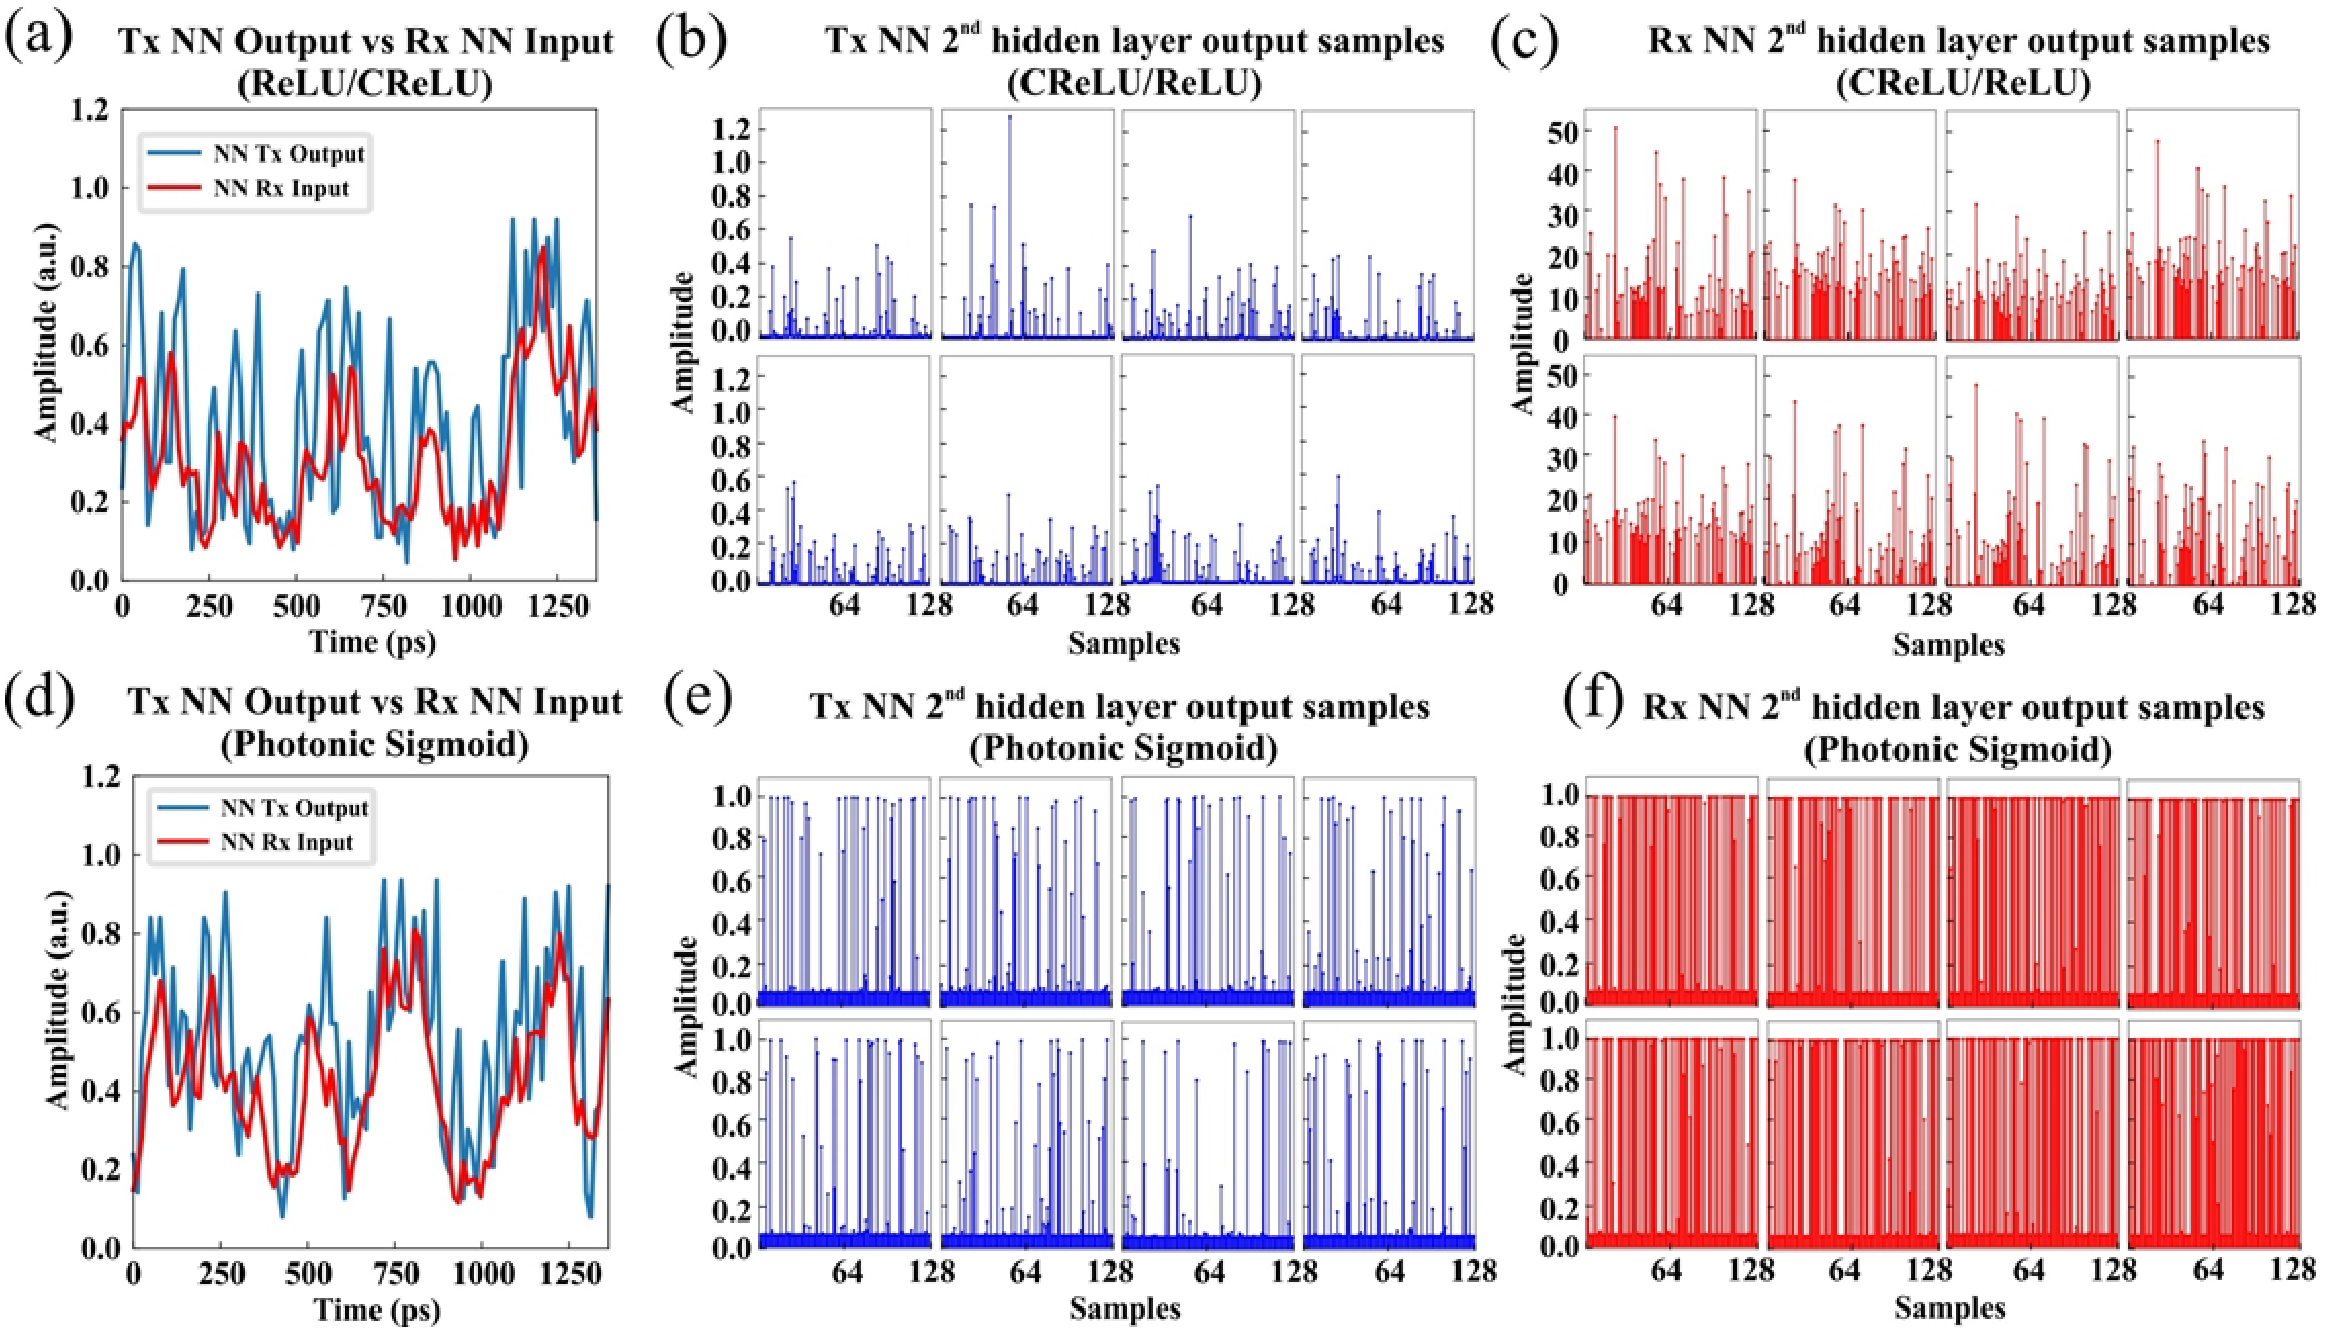
\includegraphics[width=0.5\linewidth]{sections/6_conclusions/images/experimental_analysis.jpeg}
%   \scriptsize{\textbf{\underline{Source:}} Roumpos, I., De Marinis, L., \textbf{Kirtas, M.}, Passalis, N., Tefas,
%       A., Contestabile, G., Pleros, N., Moralis-Pegios, M. and Vyrsokinos, K., 2023. \href{https://opg.optica.org/oe/fulltext.cfm?uri=oe-31-12-20068&id=531138}{High-performance end-to-end deep learning IM/DD link using optics-informed neural networks}. Optics Express}
%   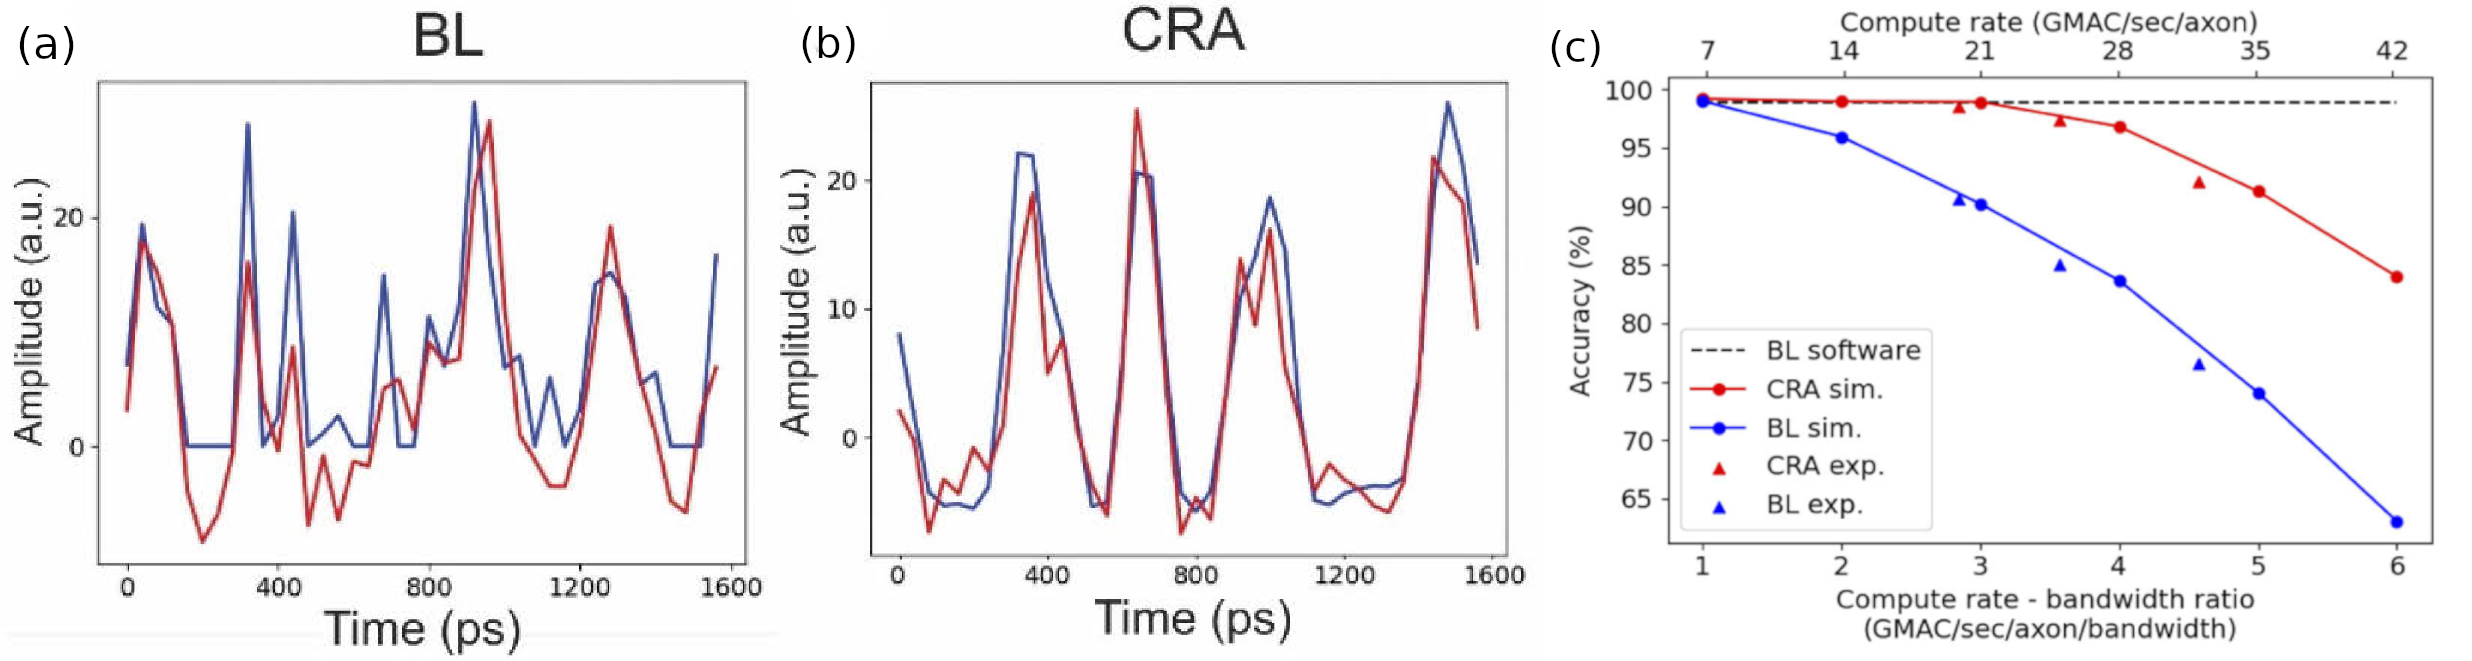
\includegraphics[width=\linewidth]{sections/6_conclusions/images/channel_overview.png}
%   \scriptsize{\textbf{\underline{Source:}} Mourgias-Alexandris, G., Moralis-Pegios, M., Tsakyridis, A., Passalis, N.,
%   \textbf{Kirtas, M.}, Tefas, A., Rutirawut, T., Gardes, F.Y. and Pleros, N., 2022. \href{https://opg.optica.org/oe/fulltext.cfm?uri=oe-30-7-10664&id=470426}{Channel response-aware photonic neural network accelerators for high-speed inference through bandwidth-limited optics.} Optics Express}
%   \end{center}
% \end{frame}

% \begin{frame}{Applications: Early DDoS Detection}
% \end{frame}

% \begin{frame}{Frame Title}
    
% \end{frame}

\begin{frame}{}
  \begin{center}
        \vspace{2cm}\\
        \textbf{Thank you!}
        \vspace{3cm}\\


        \begin{columns}
          \begin{column}{0.2\textwidth}
            
\includegraphics[width=1.2\linewidth]{./images/SYMPHONY-LOGO.png}
          \end{column}
          \begin{column}{0.39\textwidth}
            \scriptsize{This work is partially funded by SYMPHONY. The SYMPHONY project has
            received funding from Horizon Europe, the European Union’s Framework
            Programme for Research and Innovation,under grant agreement
            101135523.}
          \end{column}
          \begin{column}{0.15\textwidth}
            
\includegraphics[width=\linewidth]{./images/european-union-logo-png_seeklogo-50235.png}
          \end{column}
        \end{columns}
    \end{center}
\end{frame}


\end{document}
